% Options for packages loaded elsewhere
\PassOptionsToPackage{unicode}{hyperref}
\PassOptionsToPackage{hyphens}{url}
%
\documentclass[
  12pt,
  12pt,
  openright,
  oneside,
  a4paper,
  chapter=TITLE,
  section=TITLE,
  subsection=TITLE,
  subsubsection=TITLE,
  english,
  portugues,
  sumario=tradicional]{abntex2}
\usepackage{amsmath,amssymb}
\usepackage{lmodern}
\usepackage{iftex}
\ifPDFTeX
  \usepackage[T1]{fontenc}
  \usepackage[utf8]{inputenc}
  \usepackage{textcomp} % provide euro and other symbols
\else % if luatex or xetex
  \usepackage{unicode-math}
  \defaultfontfeatures{Scale=MatchLowercase}
  \defaultfontfeatures[\rmfamily]{Ligatures=TeX,Scale=1}
\fi
% Use upquote if available, for straight quotes in verbatim environments
\IfFileExists{upquote.sty}{\usepackage{upquote}}{}
\IfFileExists{microtype.sty}{% use microtype if available
  \usepackage[]{microtype}
  \UseMicrotypeSet[protrusion]{basicmath} % disable protrusion for tt fonts
}{}
\makeatletter
\@ifundefined{KOMAClassName}{% if non-KOMA class
  \IfFileExists{parskip.sty}{%
    \usepackage{parskip}
  }{% else
    \setlength{\parindent}{0pt}
    \setlength{\parskip}{6pt plus 2pt minus 1pt}}
}{% if KOMA class
  \KOMAoptions{parskip=half}}
\makeatother
\usepackage{xcolor}
\IfFileExists{xurl.sty}{\usepackage{xurl}}{} % add URL line breaks if available
\IfFileExists{bookmark.sty}{\usepackage{bookmark}}{\usepackage{hyperref}}
\hypersetup{
  pdfauthor={Jackson da Silva Torres},
  hidelinks,
  pdfcreator={LaTeX via pandoc}}
\urlstyle{same} % disable monospaced font for URLs
\usepackage{longtable,booktabs,array}
\usepackage{calc} % for calculating minipage widths
% Correct order of tables after \paragraph or \subparagraph
\usepackage{etoolbox}
\makeatletter
\patchcmd\longtable{\par}{\if@noskipsec\mbox{}\fi\par}{}{}
\makeatother
% Allow footnotes in longtable head/foot
\IfFileExists{footnotehyper.sty}{\usepackage{footnotehyper}}{\usepackage{footnote}}
\makesavenoteenv{longtable}
\usepackage{graphicx}
\makeatletter
\def\maxwidth{\ifdim\Gin@nat@width>\linewidth\linewidth\else\Gin@nat@width\fi}
\def\maxheight{\ifdim\Gin@nat@height>\textheight\textheight\else\Gin@nat@height\fi}
\makeatother
% Scale images if necessary, so that they will not overflow the page
% margins by default, and it is still possible to overwrite the defaults
% using explicit options in \includegraphics[width, height, ...]{}
\setkeys{Gin}{width=\maxwidth,height=\maxheight,keepaspectratio}
% Set default figure placement to htbp
\makeatletter
\def\fps@figure{htbp}
\makeatother
\setlength{\emergencystretch}{3em} % prevent overfull lines
\providecommand{\tightlist}{%
  \setlength{\itemsep}{0pt}\setlength{\parskip}{0pt}}
\setcounter{secnumdepth}{5}
%\usepackage{geometry}


% Pacotes básicos 
% ----------------------------------------------------------
%\usepackage{lmodern}			% Usa a fonte Latin Modern			
\usepackage[utf8]{inputenc}		% Codificacao do documento (conversão automática dos acentos)
\usepackage{csquotes}
\usepackage[T1]{fontenc}		% Selecao de codigos de fonte.
\usepackage{lastpage}			% Usado pela Ficha catalográfica
\usepackage{indentfirst}		% Indenta o primeiro parágrafo de cada seção.
\usepackage{color}		    	% Controle das cores
\usepackage{graphicx}			% Inclusão de gráficos
\usepackage{microtype} 			% para melhorias de justificação
\usepackage{ifthen}		    	% para montar condicionais
%\usepackage[brazil]{babel}		% para utilizar termos em portugues
\usepackage[final]{pdfpages}    % para incluir páginas de arquivos pdf
\usepackage{lipsum}				% para geração de dummy text
\usepackage{csquotes}

%\usepackage[style=long]{glossaries}
%\usepackage{abntex2glossaries}

% permite representar o cancelamento de termos em texto ou equacoes
\usepackage{cancel} 		
% cores extendidas
\usepackage{xcolor} 		
% gera diagramas a partir de listas
\usepackage{smartdiagram}   
% Para a figura ficar na posição correta
\usepackage{float} 		    
% supporte para fontes da Text Companion 
\usepackage{textcomp} 		
% uso de longtable
\usepackage{longtable}		
% simbolos matematicos
\usepackage{amsmath}	
% páginas em paisagem
\usepackage{lscape}
% mescla de colunas em tabelas
\usepackage{multicol}
% mescla de linhas em tabelas
\usepackage{multirow}
% criação do indice de quadros
\usepackage{newfloat} 
% configura legenda 
\usepackage{caption} 		
%[format=plain]
	%\renewcommand\caption[1]{%
    \captionsetup{font=small}	% tamanho da fonte 10pt
    %,format=hang
 	% \caption{#1}}
	%\captionsetup{width=0.8\textwidth}
	
%\usepackage{scrpage2}

% Pacotes de citações BibLaTeX
% ----------------------------------------------------------
\usepackage[
style=abnt,
%backref=true,
backend=biber,
maxcitenames=3,
%citecounter=true,
%backrefstyle=three,
nohashothers=true
]{biblatex}


\DefineBibliographyStrings{brazil}{%
 backrefpage = {Citado \arabic{citecounter} vez na página},% originally "cited on page"
 backrefpages = {Citado \arabic{citecounter} vezes nas páginas},% originally "cited on pages"
}

% ----------------------------------------------------------

% alterando o aspecto da cor azul
\definecolor{blue}{RGB}{55,10,249}

% ----------------------------------------------------------
\PrepareListOf{quadro}{%
\renewcommand{\cftfigpresnum}{Quadro~}}

\DeclareFloatingEnvironment[
fileext=loq,
listname={\textbf{LISTA DE QUADROS}},
name=Quadro,
%placement=p,
within= none, % numeracao continua
%within=section, % numeracao reinicia em cada seccao
%chapterlistsgaps=off
]{quadro}

\newlistentry{quadro}{loq}{0}


% Customize ‘List of Diagrams’
\PrepareListOf{quadro}{%
\renewcommand{\cftquadropresnum}{\normalsize{QUADRO}~}
\setlength{\cftquadronumwidth}{3.2cm}
%\renewcommand{\cftquadroname}{\quadroname\space} 
\renewcommand*{\cftquadroaftersnum}{\hfill--\hfill}
}

\makeatletter
%% we define a helper macro for adjusting lists of new floats to
%% accept a * behind them for not being shown in the TOC, like
%% the other list printing commands in memoir
\newcommand{\AdjustForMemoir}[1]{%
  \csletcs{kept@listof#1}{listof#1}%
  \csdef{listof#1}{%
    \@ifstar
     {\csappto{newfloat@listof#1@hook}{\append@star}%
      \csuse{kept@listof#1}}%
     {\csuse{kept@listof#1}}%
  }
}
\def\append@star#1{#1*}
\makeatother


\AdjustForMemoir{quadro} % prepare `\listofdirfigures` so it accepts a *

\makeatletter
\let\oldcontentsline\contentsline
\def\contentsline#1#2{%
    \expandafter\ifx\csname l@#1\endcsname\l@section
	\expandafter\@firstoftwo
	\else
	\expandafter\@secondoftwo
	\fi
	{%
		\oldcontentsline{#1}{\MakeTextUppercase{#2}}%
	}{%
	\normalsize %ajusta tamanho da fonte na lista
	\oldcontentsline{#1}{#2}%
}%
}
\makeatother

% Ajusta indentação de Referencias no ToC
% ----------------------------------------------------------
\defbibheading{bay}[\bibname]{%
  \chapter*{#1}%
  \markboth{#1}{#1}%
  \addcontentsline{toc}{chapter}
  {\protect\numberline{}\bibname}
}

\makeatletter
\pretocmd{\chapter}{\addtocontents{toc}{\protect\addvspace{-5\p@}}}{}{}
\pretocmd{\section}{\addtocontents{toc}{\protect\addvspace{2\p@}}}{}{}
\makeatother



%%%%%%%%%%%%%%% ALTERADO

% para citar tabelas e figuras no texto
\usepackage{hyperref}
\usepackage{varioref}

%%% auxiliar para kable

\usepackage{booktabs}
\usepackage{longtable}
\usepackage{array}
\usepackage{multirow}
\usepackage{wrapfig}
\usepackage{float}
\usepackage{colortbl}
\usepackage{pdflscape}
\usepackage{tabu}
\usepackage{threeparttable}
\usepackage{threeparttablex}
\usepackage[normalem]{ulem}
\usepackage{makecell}


%%%%%%%% Parágrafo

%\usepackage{fancyhdr}

%\usepackage{subcaption}
%\usepackage{booktabs}


%%%%%%% ESPAÇAMENTO 

%\usepackage{setspace}


%%%%%%%%%%%%%%%%%%%%%%%%%%%%%%%%%%%%%%%%%%%%%%%%%%%%%%%
% Arquivo para entrada de dados para a parte pré textual
%%%%%%%%%%%%%%%%%%%%%%%%%%%%%%%%%%%%%%%%%%%%%%%%%%%%%%%
% 
% Basta digitar as informações indicidas, no formato 
% apresentado.
%
%%%%%%%
% Os dados solicitados são, na ordem:
%
% tipo do trabalho
% componentes do trabalho 
% título do trabalho
% nome do autor
% local 
% data (ano com 4 dígitos)
% orientador(a)
% coorientador(a)(as)(es)
% arquivo com dados bibliográficos
% instituição
% setor
% programa de pós gradução
% curso
% preambulo
% data defesa
% CDU
% errata
% assinaturas - termo de aprovação
% resumos & palavras chave
% agradecimentos
% dedicatoria
% epígrafe


% Informações de dados para CAPA e FOLHA DE ROSTO
%----------------------------------------------------------------------------- 
\tipotrabalho{Dissertação}

% Marcar Sim para as partes que irão compor o documento pdf
%----------------------------------------------------------------------------- 
 \providecommand{\terCapa}{Sim}
 \providecommand{\terFolhaRosto}{Sim}
 \providecommand{\terTermoAprovacao}{Nao}
 \providecommand{\terDedicatoria}{Nao}
 \providecommand{\terFichaCatalografica}{Nao}
 \providecommand{\terEpigrafe}{Nao}
 \providecommand{\terAgradecimentos}{Nao}
 \providecommand{\terErrata}{Nao}
 \providecommand{\terListaFiguras}{Sim}
 \providecommand{\terListaTabelas}{Sim}
 \providecommand{\terSiglasAbrev}{Nao}
 \providecommand{\terResumos}{Nao}
 \providecommand{\terSumario}{Sim}
 \providecommand{\terAnexo}{Nao}
 \providecommand{\terApendice}{Nao}
 \providecommand{\terIndiceR}{Nao}
%----------------------------------------------------------------------------- 

\titulo{Efeitos das variações dos componentes do \emph{Spread} na rentabilidade das instituições bancárias através da análise de dados em painel
}
\autor{}
\local{Curitiba}
\data{2020} %Apenas ano 4 dígitos

% Orientador ou Orientadora
\orientador{}
%Prof Emílio Eiji Kavamura, MSc}
\orientadora{
Prof\textordfeminine~Dra. Mayla Costa}
% Pode haver apenas uma orientadora ou um orientador
% Se houver os dois prevalece o feminino.

% Em termos de coorientação, podem haver até quatro neste modelo
% Sendo 2 mulhere e 2 homens.
% Coorientador ou Coorientadora
\coorientador{}%Prof Morgan Freeman, DSc}
\coorientadora{}

% Segundo Coorientador ou Segunda Coorientadora
\scoorientador{}
%Prof Jack Nicholson, DEng}
\scoorientadora{}
%Prof\textordfeminine~Ingrid Bergman, DEng}
% ----------------------------------------------------------
%\addbibresource{10-references/referencias.bib}
%\bibliography{10-references/referencias.bib}
% ----------------------------------------------------------
\instituicao{Universidade Federal do Paraná}

\def \ImprimirSetor{Departamento de Economia}%
%Setor de Tecnologia}

\def \ImprimirProgramaPos{Programa Profissional de Pós-Graduação em Economia}

\def \ImprimirCurso{Mestrado Profissional em Economia}

\preambulo{
Trabalho apresentado como requisito parcial para a obtenção do título de Mestre Profisisonal em Economia no curso de Mestrado Profissional em Economia pelo Departamento de Economia da Universidade Federal do Paraná}
%do grau de Bacharel em Expressão Gráfica no curso de Expressão Gráfica, Setor de Exatas da Universidade Federal do Paraná}

%----------------------------------------------------------------------------- 

\newcommand{\imprimirCurso}{}
%Programa de P\'os Gradua\c{c}\~ao em Engenharia da Constru\c{c}\~ao Civil}

\newcommand{\imprimirDataDefesa}{
31 de Dezembro de 2020}

\newcommand{\imprimircdu}{
02:141:005.7}

% ----------------------------------------------------------
\newcommand{\imprimirerrata}{

\vspace{\onelineskip}


\begin{table}[htb]
\center
\footnotesize
\begin{tabular}{|p{1.4cm}|p{1cm}|p{3cm}|p{3cm}|}
  \hline
   \textbf{Folha} & \textbf{Linha}  & \textbf{Onde se lê}  & \textbf{Leia-se}  \\
    \hline
    1 & 10 & auto-conclavo & autoconclavo\\
   \hline
\end{tabular}
\end{table}}

% Comandos de dados - Data da apresentação
\providecommand{\imprimirdataapresentacaoRotulo}{}
\providecommand{\imprimirdataapresentacao}{}
\newcommand{\dataapresentacao}[2][\dataapresentacaoname]{\renewcommand{\dataapresentacao}{#2}}

% Comandos de dados - Nome do Curso
\providecommand{\imprimirnomedocursoRotulo}{}
\providecommand{\imprimirnomedocurso}{}
\newcommand{\nomedocurso}[2][\nomedocursoname]
  {\renewcommand{\imprimirnomedocursoRotulo}{#1}
\renewcommand{\imprimirnomedocurso}{#2}}


% ----------------------------------------------------------
\newcommand{\AssinaAprovacao}{

\assinatura{%\textbf
   {Professora} \\ UFPR}
   \assinatura{%\textbf
   {Professora} \\ ENSEADE}
   \assinatura{%\textbf
   {Professora} \\ TIT}
   %\assinatura{%\textbf{Professor} \\ Convidado 4}
      
   \begin{center}
    \vspace*{0.5cm}
    %{\large\imprimirlocal}
    %\par
    %{\large\imprimirdata}
    \imprimirlocal, \imprimirDataDefesa.
    \vspace*{1cm}
  \end{center}
  }
  
% ----------------------------------------------------------
%\newcommand{\Errata}{%\color{blue}
%Elemento opcional da \textcite[4.2.1.2]{NBR14724:2011}. Exemplo:
%}

% ----------------------------------------------------------
\newcommand{\EpigrafeTexto}{%\color{blue}
\textit{Texto}
}

% ----------------------------------------------------------
\newcommand{\ResumoTexto}{%\color{blue}

}

\newcommand{\PalavraschaveTexto}{%\color{blue}
latex. abntex. editoração de texto.}

% ----------------------------------------------------------
\newcommand{\AbstractTexto}{%\color{blue}
This is the english abstract.
}
% ---
\newcommand{\KeywordsTexto}{%\color{blue}
latex. abntex. text editoration.
}

% ----------------------------------------------------------
\newcommand{\Resume}
{%\color{blue}
Il s'agit d'un résumé en français.
} 
% ---
\newcommand{\Motscles}
{%\color{blue}
 latex. abntex. publication de textes.
}

% ----------------------------------------------------------
\newcommand{\Resumen}
{%\color{blue}
Este es el resumen en español.
}
% ---
\newcommand{\Palabrasclave}
{%\color{blue}
latex. abntex. publicación de textos.
}

% ----------------------------------------------------------
\newcommand{\AgradecimentosTexto}{%\color{blue}

}

% ----------------------------------------------------------
\newcommand{\DedicatoriaTexto}{%\color{blue}
\textit{}
	}


\makeindex
\usepackage{helvet}
\renewcommand{\familydefault}{\sfdefault}
\DeclareUnicodeCharacter{0301}{******}
\DeclareUnicodeCharacter{0303}{******}
\DeclareUnicodeCharacter{0327}{******}
\DeclareUnicodeCharacter{0308}{******}
\usepackage{booktabs}
\usepackage{longtable}
\usepackage{array}
\usepackage{multirow}
\usepackage{wrapfig}
\usepackage{float}
\usepackage{colortbl}
\usepackage{pdflscape}
\usepackage{tabu}
\usepackage{threeparttable}
\usepackage{threeparttablex}
\usepackage[normalem]{ulem}
\usepackage{makecell}
\usepackage{xcolor}
\ifLuaTeX
  \usepackage{selnolig}  % disable illegal ligatures
\fi
\usepackage[]{biblatex}

\author{Jackson da Silva Torres}
\date{2021}

\begin{document}

\ifthenelse{\equal{\terCapa}{Sim}}{
\imprimircapa}{}

\ifthenelse{\equal{\terFolhaRosto}{Sim}}{
\imprimirfolhaderosto*}{}

\ifthenelse{\equal{\terFichaCatalografica}{Sim}}{
 \insereFichaCatalografica{}\cleardoublepage}{
 }

\ifthenelse{\equal{\terErrata}{Sim}}{
 \begin{errata}%\color{blue}
   \imprimirerrata
  \end{errata}}{
  }

\ifthenelse{\equal{\terTermoAprovacao}{Sim}}{
\insereAprovacao}{}

\ifthenelse{\equal{\terDedicatoria}{Sim}}{
\begin{dedicatoria}
   \vspace*{\fill}
   \centering
   \noindent
   \DedicatoriaTexto
   \vspace*{\fill}
\end{dedicatoria}
}{
}

\ifthenelse{\equal{\terAgradecimentos}{Sim}}{
 \begin{agradecimentos}
    \AgradecimentosTexto
  \end{agradecimentos}
  }{
  }

\ifthenelse{\equal{\terEpigrafe}{Sim}}{
\begin{epigrafe}
    \vspace*{\fill}
    \begin{flushright}
        \EpigrafeTexto
    \end{flushright}
\end{epigrafe}
}{}

\ifthenelse{\equal{\terResumos}{Sim}}{
\begin{resumo}
    \ResumoTexto
    

   \noindent 
   \textbf{Palavras-chaves}: \PalavraschaveTexto
\end{resumo}

\begin{resumo}[ABSTRACT]
 \begin{otherlanguage*}{english}
   \AbstractTexto
   
   \noindent 
   \textbf{Key-words}: \KeywordsTexto
 \end{otherlanguage*}
\end{resumo}

}{}

\ifthenelse{\equal{\terListaFiguras}{Sim}}{
\pdfbookmark[0]{\listfigurename}{lof}
\listoffigures*
\cleardoublepage
}{}

\ifthenelse{\equal{\terListaGraficos}{Sim}}{
\listofgrafico*
\cleardoublepage
}{}

\ifthenelse{\equal{\terListaQuadros}{Sim}}{
\listofqdr*
\cleardoublepage
}{}

\ifthenelse{\equal{\terListaTabelas}{Sim}}{
\listoftables*
\cleardoublepage
}{}

\ifthenelse{\equal{\terSiglasAbrev}{Sim}}{
    \imprimirlistadesiglas
    \cleardoublepage
    \imprimirlistadesimbolos
    \cleardoublepage
 }{}

\ifthenelse{\equal{\terSumario}{Sim}}{
\pdfbookmark[0]{\contentsname}{toc}
\tableofcontents*
\cleardoublepage
}{}

\textual
\pagestyle{simple}
\parindent 1.50cm

\chapter[INTRODUÇÃO]{INTRODUÇÃO}

Esta pesquisa tem a proposição de averiguar os aspectos técnicos fundamentais sobre mercado bancário brasileiro em função dos determinantes do \emph{spread} e suas influências na rentabilidade bancária, através de abordagem teórica, analítica e aplicada.

\section{Estrutura}

A presente dissertação estará estruturada em três capítulos. Este primeiro apresenta a presente estrutura do trabalho contextualização, objetivos e a justificativa. Esta estrutura visa sintetizar as principais questões sobre o tema proposto com ótica direcionada para a proposição e objetivos, bem como nortear o andamento da pesquisa.

No segundo capítulo será construído o referencial teórico contemplando os aspectos fundamentais e dados amplos a respeito do setor bancário e \emph{spread} no Brasil, por meio de pesquisa bibliográfica e busca em bancos de dados. Bem como apresentrar as principais pesquisas sobre o \emph{spread} bancário.

O terceiro capítulo trará a construção dos procedimentos metodologicos para seleção e execução do modelo econométrico a ser empregado para a avaliação dos efeitos dos determinantes do \emph{spread} simultaneamente no \emph{spread ex-post} e na rentabilidade bancária.

No quarto capítulo se almeja explanar e analisar, diante as premissas empregadas, os resultados obtidos no modelo, conforme planejado no capítulo terceiro, visando descrever e embasar as relações entre as variáveis, confrontando com as pesquisas identificadas.

Por fim serão realizadas as considerações finais, buscando contextualizar os resultados obtidos com o cenário e os estudos identificados e sugerindo estudos complementares.

\section{Contextualização}

Ao longo da histórica, os instrumentos financeiros passaram por profundas modificações e evoluções, assumindo papel determinante na geração e acúmulo de riqueza para as famílias e nações. E nesse contexto histórico, durante o renascimento, as atividades de negociação de dinheiro e câmbio de moeda estranheira se formalizaram, surgindo o que viriam a se tornar as primeiras instituições bancárias.

Na contrapartida destas atividades, as instituições bancárias são remuneradas basicamente de duas formas. A primeira delas é através de taxas sobre os serviços envolvendo a custódia. A segunda se dá pelo valor oriundo da cobrança de uma taxa de juros sobre o capital de emprestado, configurando assim o \emph{spread} bancário \cite{leite:1996, campello:2005, neves:2007}.

A medida que a oferta de crédito desponta como um fator fundamental para o desenvolvimento econômico de longo prazo, incentivando empreendimentos produtivos, contribuindo com a geração de emprego, renda e lucros, o \emph{spread} bancário passa a ser um indicador estratégico para determinação do nível de desenvolvimento de países e regiões \cite{WB:2005, levine:1997}.

A primeira via da importância do \emph{spread} bancário está relacionada com a
solidez do sistema financeiro. O nível deste indicador deve ser suficiente para
garantir lucros atrativos, fazendo que as instituições mantenham suas
atividades e que novas tenham interesse em entrar no mercado, resultando em um
setor forte, com segurança e liquidez \cite{levine:1997, dantas:2012, leal:2006}.

A segunda via, remete a relação entre o \emph{spread} e o nível de atividade
econômica. Segundo estudos recentes, um elevado nível de \emph{spread} bancário
desfavoreceria o crédito produtivo e consequentemente o nível de atividade
econômica, impactando no crescimento e desenvolvimento do país ou região \cite{WB:2005, dantas:2012, leal:2006}.

Tais premissas são sustentadas pelo Fundo Monetário Internacional (FMI) e Banco Mundial (BM), que realizam e incentivam estudos sobre o indicador a nível mundial. A grande maioria dos estudos demonstram a relação inversa entre a taxa de \emph{spread} bancário e os indicadores de desenvolvimento dos países e regiões \cite{WB:2005}.

Estudos constataram que a América Latina possui as maiores taxas de juros, bancos mais ineficientes, implicando assim em níveis de \emph{spread} elevados. Dentre os países da América Latina, o caso brasileiro é destacado como o cenário mais crítico, com níveis de lucros considerados elevados, afetando principalmente o setor produtivo \cite{dantas:2012}.

Entre diversos países estudados, desde a década de 1990, é evidenciado o caso brasileiro com elevados níveis de \emph{spread} bancário, baixa relação entre crédito e PIB e cenários de crescimento econômicos instáveis e considerados baixos \cite{levine:1997, matos:2003}. Mesmo com recentes modificações no cenário, o caso brasileiro desperta constantes iniciativas de estudos.

Durante a década de 1990, o \emph{spread} bancário brasileiro esteve superior a 50\% a.a., enquanto na América Latina o observado foi entre 10\% e 15\% a.a.. A relação crédito/PIB no Brasil, em 2003, era de 23\%, considerado muito baixo em comparação ao Chile com 68,5\%, Uruguai com 64,3\%, Estados Unidos com 60,8\%, Japão com 64,3\%, Coréia com 98,9\% e Europa com 140,6\% \cite{camargo:2009, singh:2005}.

Observa-se assim, a relevância do estudo acerca das variáveis que influenciam o \emph{spread} bancário \emph{ex-post} no Brasil. Sendo assim, esta pesquisa parte das indagações: (1) Quais variáveis endógenas e exógenas exercem influência significativa no \emph{spread} bancário \emph{ex-post} e (2) como os determinantes dos \emph{spread} afetam o \emph{spread ex-post} e a rentabilidade das instituições bancárias no Brasil?

\section{Objetivos}

\subsection{Objetivo Geral}

Este estudo buscará investigar variáveis microeconômicas e macroeconômicas que exerçam influência significativa sobre o \emph{spread ex-post} e como estas afetaram a rentabilidade das instituições bancárias brasileiras, entre março de 2011 e novembro de 2020.

\subsection{Objetivos Específicos}

\begin{enumerate}
\def\labelenumi{\arabic{enumi}.}
\tightlist
\item
  Realizar o mapeamento e sistematização de aspectos teóricos e técnicos sobre o setor bancário e \emph{spread} no Brasil;
\item
  Identificar e testar variáveis macroeconômicas e microeconômicas enquanto componentes implícitos e explícitos de determinação do \emph{spread} bancário \emph{ex-post};
\item
  Analisar como as variações das variáveis determinantes do \emph{spread} bancário afetaram a rentabilidade dos bancos.
\end{enumerate}

\section{Justificativa teórica e prática}

A medida que o nível de dinamismo da economia se eleva, ocorrendo evoluções e modificações estruturais em espaços de tempo mais curtos, o setor financeiro deve acompanhar tais perspectivas, devido sua importância no processo, principalmente no que se refere ao oferecimento de novos produtos, ampliação de crédito, oportunidades para investidores, solidez e liquidez ao sistema.

E nesse cenário dinâmico e evolutivo, o \emph{spread} bancário desponta como o indicador que capta o nível de desenvolvimento do sistema financeiro, no sentido de equacionar a relação entre a remuneração dos superavitários e os juros cobrados dos deficitários de capital, englobando os custos de intermediação, com maior relevância aos créditos destinados a empreendimentos produtivos.

Nesse sentido, os estudos acerca do \emph{spread} bancário se tornam necessários e importantes, diante da perspectiva do dinamismo e constantes transformações na economia. O caso brasileiro demonstra ser ainda mais relevante, por se colocar em posição considerada peculiar, diante os históricos de baixo crescimento e desenvolvimento e um setor bancário concentrado com elevados níveis de \emph{spread}.

Foi verificado o panorama das publicações de pesquisas relacionadas ao setor bancário no brasil, através da plataforma Capes, entre os anos 2000 e 2020
\footnote{Foram utilizados operadores booleanos em inglês: banking(structure or
market or sector or industry) and brazil* e revisados por pares.}, remontando um total de 4.512 publicações, indicando a relevância do tema. Enquanto as pesquisas relacionadas especificamente com o \emph{spread} bancário brasileiro, através da plataforma Capes foram identificados 3.435 estudos entre os anos de 2000 e 2020 \footnote{Foram utilizados os operadores boleanos em
inglês (bank or banking) and spread and brazil, revisados por pares.}, o que também vem destacar a importância da temática na literatura acadêmica.

Mesmo com um número considerado de estudos sobre o setor bancário brasileiro e outros diversos citando o \emph{spread} bancário, ainda se fazem necessárias novas iniciativas, diante a importância deste indicador na solidez do setor financeiro e seu papel no desenvolvimento econômico, e principalmente por ainda existirem incongruências, divergências entre resultados e lacunas sobre determinantes a serem explanadas.

Este trabalho atuará em duas perspectivas que tangem os estudos acerca do \emph{spread} bancário. A primeira está moldada na consensual importância do \emph{spread} no processo de desenvolvimento econômico via concessão de crédito, o que traz a importância de verificar suas variáveis determinantes. A segunda, parte da importância de um nível de rentabilidade bancária que proporcione um sistema financeiro sustentável.

O próximo capítulo irá abordar sobre aspectos conceituais, teóricos, técnicos e históricos do setor e \emph{spread} bancário brasileiro, buscando demonstrar as principais características deste mercado, através da descrição e demonstração da evolução da estrutura e seus principais indicadores.

\textual
\pagestyle{simple}

\parindent 1.50cm

\chapter{Referencial Teórico}

Este capítulo se configura no referencial teórico acerca de conceitos e aspectos técnicos fundamentais envolvendo o setor bancário e o \emph{spread} bancário no Brasil. A primeira seção irá abordar sobre a estrutura e evolução do setor bancário brasileiro. A segunda seção abordará sobre os conceitos técnicos, teóricos e estudos sobre \emph{spread} bancário.

\section{Setor Bancário no Brasil}

Nesta seção serão abordados os conceitos, características, composição e evolução do setor bancário brasileiro, com objetivo de identificar variáveis quantitativas e qualitativas relevantes para as análises dos componentes e determinantes do \emph{spread} bancário. A primeira parte trará um breve histórico do mercado bancário, e a segunda parte sobre conceitos e evolução de dados.

O sistema financeiro exerce papel socioeconômico fundamental, atuando na intermediação, promoção da circulação do fluxo de crédito, disponibilização de meios de pagamentos e opções para alocação de recursos, investimentos, seguros, transações cambiais, operações de proteção de capital, guardando relação com grau de desenvolvimento econômico de um país ou região \cite{maffili:2009}.

Devido a importância de um sistema financeiro sólido no desenvolvimento econômico, os lucros auferidos no setor despertam constantes atenções, girando em torno dos riscos que envolvem descontinuidade e insolvência \cite{couto:2002}. De acordo com Freitas e Khöler (2009) \emph{apud} \textcite{dantas:2012}, o Brasil apresenta uma conjuntura bancária peculiar em comparação a outros países, principalmente no que se refere aos lucros.

Esta observação remete ao conceito que o desenvolvimento do setor bancário em cada país e região pode ser influenciado por diversos fatores endógenos --- relacionados com a gestão, tecnologia e eficiência de cada instituição --- e exógenos --- envolvendo a regulação e as conjunturas econômica e social \cite{rover:2011}.

\subsection{Aspectos históricos}

A história bancária no Brasil tem sua ``pedra fundamental'' com a instituição, em 1808, do Banco do Brasil, em virtude da chegada da família real portuguesa e as medidas de aberturas dos portos e acordos comercias. A instituição teve suas atividades encerradas em 1829, devido a uma série de prejuízos com exportações e ao retorno de D. João VI à Portugal, levando maior parte do lastro metálico \cite{costaneto:2004, camargo:2009}.

No ano de 1833 o Banco do Brasil foi recriado, porém não ocorreram os aportes de capital necessários para instalação e operação. O ano de 1836 foi marcado pela fundação do Banco do Ceará, o primeiro banco comercial privado, que operou até 1839. O Banco do Brasil foi constituído pela terceira vez, agora sob controle privado, fundado pelo Barão de Mauá, no ano de 1851 \cite{costaneto:2004, camargo:2009}.

Em 1853 o Banco do Brasil realizou a primeira operação fusão do país, com o Banco Comercial do Rio de Janeiro, criado em 1838, considerada a quarta versão desta instituição \cite{camargo:2009}. O Banco do Brasil da atualidade tem sua origem em 1906, resultante do decreto nº 1.455 de 30/12/1905, que autorizou a fusão do Banco do Brasil de 1853 com o Banco da República do Brasil \cite{camargo:2009, Lei:1455:1905, costaneto:2004}.

No ano de 1863 foram instalados o primeiros bancos estrangeiros, sendo eles o London \& Brazilian Bank e The Brazilian and Portuguese Bank, ambos com sede no Rio de Janeiro. Posteriormente os bancos estrangeiros passaram a dominar o mercado. A conjuntura nesse momento ainda não se configurava como sistema bancário desenvolvido, em termos de integração entre as instituições \cite{camargo:2009, guimaraes:2011, mendes:2014}.

A Lei Bancária de 1921 trouxe um grande movimento para nacionalização bancária e construção de um efetivo sistema financeiro. O bancos estrangeiros tiveram suas atividades limitadas, passando a serem proibidas pelas Constituições de 1934 e 1937, voltando a serem autorizadas a funcionar pela Constituição de 1946, posição reiterada pela Constituição de 1967 \cite{camargo:2009, decreto:1921, guimaraes:2011}.

O movimento para criação e fortalecimento do sistema bancário nacional iniciado na década de 1920 perdurou até o ano de 1964 com a reforma financeira que resultou no Sistema Financeiro Nacional (SFN). Esse período foi marcado pela criação de mecanismos de controle e fiscalização, fomento e expansão da rede bancária \cite{camargo:2009, guimaraes:2011}.

Entre o período de 1964 a 1980 foram implementadas diversas reformas, criações de mecanismos, instituições e subsistemas. Foram definidas modalidades e atividades, onde os Bancos Comerciais se limitariam a operações de créditos de curto prazo, enquanto os bancos de investimento e desenvolvimento atuariam na concessão de crédito de longo prazo \cite{camargo:2009}.

O setor bancário brasileiro passou por significativas transformações em sua estrutura no final da década de 1980 e ao longo da década de 1990. Estas modificações ocorreram em grande parte como reflexo às mudanças internacionais, ao processo de abertura comercial e financeira que se iniciou no Brasil, e das próprias modificações das conjunturas econômica e social \cite{camargo:2009}.

Entre as principais mudanças iniciadas na década de 1980 está a reforma bancária ocorrida em 1988, advindas da Constituição e principalmente através da Resolução nº 1.524, que instituiu diversas medidas de desregulamentação, entre elas a extinção da necessidade de carta-patente para constituição de Bancos Múltiplos \cite{Res:1524:1988}.

Alguns dos efeitos da abertura comercial-financeira e das modificações na estrutura bancária provenientes das medidas governamentais foram o aumento da participação de instituições estrangeiras no país e, um consistente processo de fusões e aquisições, de ambas as origens de capital, que resultou em considerável elevação do grau de concentração \cite{camargo:2009}.

Mesmo com as limitações impostas pela Constituição de 1988 \cite{constituicao:1988} para instalação de bancos estrangeiros, não houveram restrições para que ocorressem aumentos na participação de capital estrangeiro em bancos nacionais, comportamento esse que se tornou até os dias atuais a principal forma de participação desta instituições no Brasil \cite{camargo:2009}.

\subsection{Estrutura e evolução}

No Brasil, o Sistema Financeiro Nacional (SFN) consolidado, é composto por um conjunto de instituições e subsistemas, com a divisão em Bancos e Caixas Econômicas, Corretoras de Câmbio, Fintechs, Administradora de consórcios, Cooperativa de crédito, Instituições de pagamento, Corretora e a distribuidora e outras instituições não bancárias \cite{Lei:4595:1964}.

O setor bancário está sob hierarquia normativa do Conselho Monetário Nacional (CMN) e supervisão do Banco Central do Brasil (BACEN). As instituições que formam o setor bancário assumem o papel de operadoras no mercado de crédito, atuando como intermediadoras financeiras junto às pessoas físicas e jurídicas, podendo ser de caráter público ou privado \cite{Lei:4595:1964}.

\begin{table}[!hbtp]
\vspace{20pt}
\caption{Composição do setor bancário brasileiro por tipo de iniciativa  — Dezembro 2019}
\vspace{1mm}
\begingroup\fontsize{10}{12}\selectfont

\begin{tabu} to \linewidth {>{\raggedright\arraybackslash}p{8cm}>{\raggedright\arraybackslash}p{7cm}}
\toprule
Caráter & Participação\\
\midrule
\cellcolor{gray!6}{Privado} & \cellcolor{gray!6}{93\%}\\
Público & 7\%\\
\bottomrule
\end{tabu}
\endgroup{}
\vspace{1mm}
\label{tab:iniciativa}
\fonte{Desenvolvido pelo autor, com dados do Banco Central}
\vspace{-2mm}
\end{table}

As modalidades de instituições no setor bancário brasileiro são os Bancos
Comerciais, Bancos de Investimentos, Bancos de Desenvolvimento, Bancos de
Câmbio, Bancos Múltiplos e Caixas Econômicas. Atualmente na modalidade de Caixas Econômicas somente a Caixa Econômica Federal está em funcionamento
\cite{Lei:4595:1964, Res:2099:1994, Res:2624:1999, Res:394:1976, Res:3426:2006, DL:759:1969}.

Na \autoref{tab:banks} é possível verificar, no ano de 2019, a quantidade de instituições por modalidade com uma massiva concentração em bancos múltiplos, com 76\%,3 de participação, onde apenas 11,5\% das instituições bancárias operam exclusivamente com carteira comercial, 6,3\% exclusivamente com investimento, 2,89\% em câmbio, 2,31\% em desenvolvimento, e a Caixa econômica Federal.

\begin{table}[!hb]
\vspace{20pt}
\caption{Composição do setor bancário brasileiro por segmento em dezembro de 2019}
\vspace{1mm}
\begingroup\fontsize{10}{12}\selectfont

\begin{tabu} to \linewidth {>{\raggedright\arraybackslash}p{5cm}>{\raggedleft\arraybackslash}p{4cm}>{\raggedright\arraybackslash}p{5cm}}
\toprule
Segmento & Quantidade & Participação\\
\midrule
\cellcolor{gray!6}{Banco Múltiplo} & \cellcolor{gray!6}{132} & \cellcolor{gray!6}{76.30\%}\\
Banco Comercial & 20 & 11.56\%\\
\cellcolor{gray!6}{Banco de Investimento} & \cellcolor{gray!6}{11} & \cellcolor{gray!6}{6.36\%}\\
Banco de Câmbio & 5 & 2.89\%\\
\cellcolor{gray!6}{Banco de Desenvolvimento} & \cellcolor{gray!6}{4} & \cellcolor{gray!6}{2.31\%}\\
\addlinespace
Caixas Econômicas & 1 & 0.58\%\\
\bottomrule
\end{tabu}
\endgroup{}
\vspace{1mm}
\label{tab:banks}
\fonte{Desenvolvido com dados do Banco Central}
\vspace{-2mm}
\end{table}

Entre as características gerais na formalização das instituições bancárias, estão a obrigatoriedade de serem instituídas como sociedades anônimas, possuirem em sua denominação as nomenclaturas: banco, banco de investimento, banco de desenvolvimento, banco de câmbio, caixa econômica, conforme sua categoria \cite{Lei:4595:1964, Res:2099:1994, Res:2624:1999, Res:394:1976, Res:3426:2006, DL:759:1969}.

Os Bancos Comerciais são instituições financeiras de caráter público ou privado, atuando na intermediação de recursos financeiros de curto e médio prazo para financiamento de atividades comerciais, industriais, serviços para pessoas físicas e terceiros, realizando captações através de operações de depósitos a vista de livre movimento e depósitos a prazo \cite{Res:2099:1994}.

Na modalidade de Bancos de Investimento, as instituições devem possuir caráter privado, podendo operar participações temporárias em sociedades, financiamentos produtivos para ativo fixo e capital de giro e gestão de recursos de terceiros. Realizam captação através de depósitos a prazo, repasses externos e internos e comercialização de cotas de fundos de investimentos que administram \cite{Res:2624:1999}.

O Bancos de Desenvolvimento são instituições de caráter público, de controle federal ou estadual, com foco em financiamento de atividades que promovam o desenvolvimento econômico regional no médio e longo prazo, realizando operações passivas de depósitos a prazo, recursos externos, endossos hipotecários e operações ativas de empréstimos e financiamentos ao setor privado \cite{Res:394:1976}.

Os Bancos Múltiplos se caracterizam por instituições financeiras que podem assumir caráter público ou privado, com a autorização para realizarem operações ativas e passivas por meio do acúmulo de múltiplas carteiras, sendo elas a comercial, investimento, desenvolvimento, crédito imobiliário, arrendamento mercantil e crédito, financiamento e investimento \cite{Res:2099:1994}.

Em sua composição os Bancos Múltiplos são obrigados a assumir no mínimo duas carteiras, sendo que de forma obrigatória, uma delas deve ser ou a carteira comercial, ou a de investimento. As que optarem por carteira comercial podem realizar captação de recursos via depósito a vista, e somente os Bancos Públicos podem acumular a carteira de desenvolvimento \cite{Res:2099:1994}.

Os Bancos de Câmbio, são instituições financeiras que possuem autorização para realizar operações de compra e venda de crédito cambial. Entre as operações de crédito estão o financiamento de exportações e importações e antecipação mediante contratos cambiais. Podem captar depósitos em contas com movimentação restrita e sem remuneração, exclusivo às operações cambiais \cite{Res:3426:2006}.

A Caixa Econômica Federal (CEF), fundada em 1861, e regulamentada pelo Decreto-Lei nº 759 de 1969 é uma empresa pública subordinada ao Ministério da Economia, com operações similares a de um Banco Comercial, priorizando projetos e programas relacionados a área social e infraestrutura, detendo o monopólio sobre o penhor de bens pessoais e venda de bilhetes de loteria. \cite{DL:759:1969}.

A CEF atua com operações de crédito ao consumidor, para financiamento de bens
de consumo duráveis, operações de garantia de penhor industrial e caução de
títulos. É integrante do Sistema Financeiro da Habitação (SFH) e Sistema
Brasileiro de Poupança e Empréstimo (SBPE), além da detenção centralizado do recolhimento e aplicação dos recursos do FGTS \cite{DL:759:1969}.

O \autoref{graf:segmento} demonstra a evolução número de instituições bancárias por segmento entre 1978 à 2019, podendo ser visualizada uma mudança na composição da estrutura, com significativo aumento de instituições aderindo a modalidades de múltiplas carteiras \footnote{As primeiras instituições com carteira múltipla começaram a operar no ano de 1988} e redução de instituições que operam exclusivamente com carteira comercial e exclusivamente com carteira
de investimento.

\begin{grafico}[!htbp]
\vspace{20pt}
\caption{Evolução do setor bancário brasileiro por segmento}
\vspace{-4mm}

\begin{center}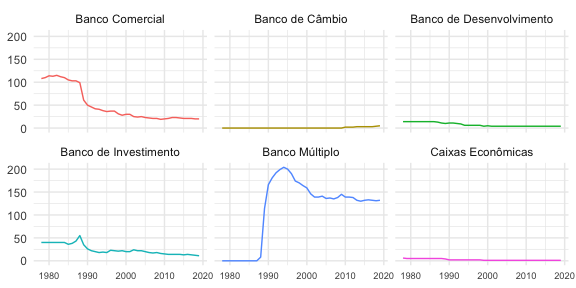
\includegraphics{12-exportedfigures/bank.evolution-1} \end{center}
\vspace{-3mm}
\label{graf:segmento}
\fonte{Desenvolvido a partir de dados do Banco Central}
\vspace{-2mm}
\end{grafico}

\subsection{Concentração Bancária}

A observação sobre o aumento da concentração bancária no Brasil, realizada por \textcite{camargo:2009}, pode ser visualizada na \autoref{graf:concentracao}. Entre as metades das décadas de 1980 e 1990, com redução da concentração, levando em consideração o número de instituições. Esse cenário passou se inverter a partir de 1994, chegando em 2019 a um nível aproximado ao observado no início da década de 1980.

\begin{grafico}[!hbtp]
\vspace{20pt}
\caption{Evolução da quantidade de instituições no setor bancário brasileiro}
\vspace{-4mm}

\begin{center}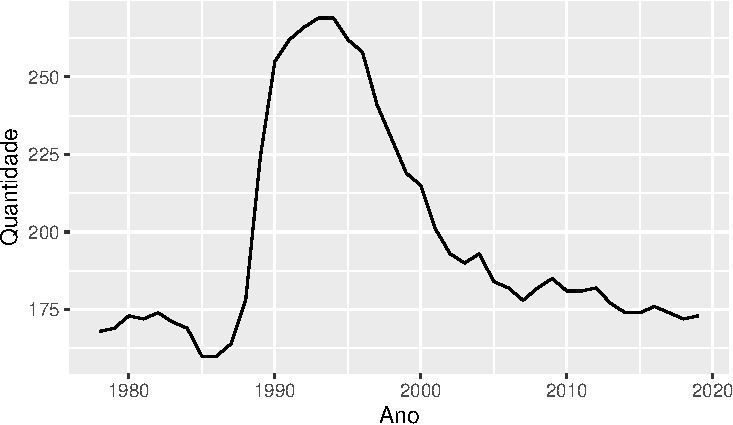
\includegraphics{12-exportedfigures/concetration-1} \end{center}
\vspace{-3mm}
\label{graf:concentracao}
\fonte{Desenvolvido pelo autor, com dados do Banco Central}
\vspace{-2mm}
\end{grafico}

O aumento da concentração bancária pode ser prejudicial ao crescimento econômico, uma vez que, com maior participação no mercado, as instituições bancárias acabam por obter a prerrogativa de determinar os preços de juros e serviços, comportamento este observado pelos autores Strachman e Vasconcelos \emph{apud} \textcite{camargo:2009} e \textcite{klein:1971}.

Segundo \textcite{camargo:2009} e \textcite{dantas:2012}, por outra perspectiva, o ganho de escala, em um cenário de aumento da participação de mercado das instituições, refletindo nas suas operações de crédito e redução de custos operacionais atuaria melhorando a remuneração dos depósitos e refletindo na redução dos juros finais pagos pelos clientes.

Outra possível tendência para a concentração bancária seria a redução do risco
das operações, implicando em redução de custos, obtida por meio expansão
geográfica, setorial e de produtos financeiros. Porém os possíveis efeitos da
concentração dependem de uma série de condições, principalmente em torno da
eficiência e do nível de concorrência no mercado \cite{camargo:2009}.

Entre os principais indicadores para medir a concentração de mercado está o índice Herfindahl--Hirschmanahl(HHI), desenvolvido pelos economistas Orris C. Herfindahl e Albert O. Hirschman. É utilizado amplamente para medidas de regulação da concorrência e leis antitrust.

O HHI tem sido utilizado como uma medida de competição e bancária em nível mundial como exposto em Santos e Kuroda (2012), e nos estudos de Rodamilans (2016), Ferreira (2016), Cardoso (2016) esta variável apresentou considerável significância estatística nos modelos propostos.

Frequentemente o HHI tem sido utilizado em modelos econométricos como variável explanatória para o nível de \emph{spread} bancário, como em \textcite{dantas:2012}, PERIA e MODY (2004) \emph{apud} \textcite{leal:2006} e \textcite{almeida:2013}, todos remontando significância estatística para esta variável.

O HHI refere-se a uma medida de concentração de mercado que mede a participação de uma determinada firma no mercado do qual participa. É obtida pela somatória quadrática da parcela de mercado a ser considerada, variando entre \(1/N\) e \(1\), conforme \autoref{eq:hhi01}.

\begin{equation}\label{eq:hhi01}
HHI = \sum_{i=1}^{N}q_i^2
\vspace{10pt}
\end{equation}

A versão normalizada do HHI traz uma variação entre \(0\) e \(1\), perdendo em seu resultado a captação diante o número de firmas, de acordo com a \autoref{eq:hhi02}

\begin{equation}\label{eq:hhi02}
HHIN = \frac{\frac{HHI - 1}{N}}{\frac{1-1}{N}}
\end{equation}

A versão decomposta do HHI, conforme \autoref{eq:hhi03}, avalia a assimetria da concentração de mercado inserindo um componente de variabilidade das participações das firmas, assim se verifica se as firmas possuem uma participação de mercado simétrica resultando em \(HHIN = 0\) e \(HHI= 1/N\), confome a \autoref{eq:hhi03}
.

\begin{equation}\label{eq:hhi03}
HHID = \frac{1}{N} + N\frac{\sum_{i=1}^{N}(\frac{q_i - 1}{N})^2}{N}
\end{equation}

\subsection{Participação estrangeira}

A elevação da participação estrangeira no setor bancário brasileiro durante a década de 1990, evidenciado por \textcite{camargo:2009} pode ser observado no \autoref{graf:ev.capital} e \autoref{tab:origemcapital}. Ocorrendo principalmente através do controle acionário, com elevação acentuada na segunda metade da década de 1990 até o início da década de 2000.

\begin{table}
\vspace{20pt}
\caption{Setor bancário brasileiro por origem de capital — Dezembro de 2019}
\vspace{1mm}
\begingroup\fontsize{10}{12}\selectfont

\begin{tabu} to \linewidth {>{\raggedright}X>{\raggedleft}X>{\raggedright}X}
\toprule
Capital & Quantidade & Participação\\
\midrule
\cellcolor{gray!6}{Nacionais} & \cellcolor{gray!6}{66} & \cellcolor{gray!6}{43.1\%}\\
Controle Estrangeiro & 60 & 39.2\%\\
\cellcolor{gray!6}{Nacionais com Participação Estrangeira} & \cellcolor{gray!6}{12} & \cellcolor{gray!6}{7.8\%}\\
Públicos & 10 & 6.5\%\\
\cellcolor{gray!6}{Estrangeiros} & \cellcolor{gray!6}{5} & \cellcolor{gray!6}{3.3\%}\\
\bottomrule
\end{tabu}
\endgroup{}
\vspace{1mm}
\label{tab:origemcapital}
\fonte{Desenvolvida pelo autor, com dados do Banco Central}
\vspace{-2mm}
\end{table}

A expectativa com o aumento de instituições nacionais com controle estrangeiro era que, houvesse elevação da concorrência e, consequentemente, redução no \emph{spread} bancário, aumento da concessão de crédito, melhoria da qualidade e dos produtos financeiros, avanços em tecnologias, ou seja, uma elevação na eficiência do setor \cite{camargo:2009}.

Porém, o que se observou foi a adoção de postura conservadora por partes dos bancos estrangeiros, com estratégia de ativos inclinada para negociação de títulos públicos, e passivos direcionados para a captação de recursos advindos de grupos de rendas média e alta, com exceção dos bancos públicos que concentraram em operações de crédito \cite{camargo:2009}.

Em estudo do \textcite{BCB:1999}, foi constatado que a participação de instituições estrangeiras no mercado nacional refletiu em uma maior eficiência operacional. E que o aumento desta participação se deu pela aquisição por parte de instituições estrangeiras de bancos bancos nacionais com problemas operacionais.

\begin{grafico}[!htbp]
\vspace{20pt}
\caption{Evolução da origem de capital das instituições bancárias no Brasil}
\vspace{-4mm}

\begin{center}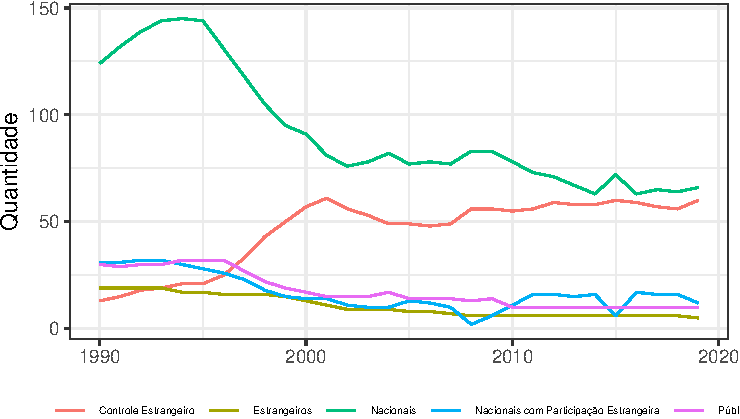
\includegraphics{12-exportedfigures/capital.graphic-1} \end{center}
\label{graf:ev.capital}
\fonte{Desenvolvido pelo autor, com dados do Banco Central}
\end{grafico}

A inclinação para aplicação massiva em títulos públicos por parte das instituições estrangeiras e de controle estrangeiro se dava diante a manutenção de elevadas taxas de juros, tornando o crédito para empreendimentos privados de elevado risco, e consequentemente elevando substancialmente o \emph{spread} bancário e reduzindo a oferta de crédito \cite{camargo:2009}.

\subsection{Indicadores de crédito}

Outra variável importante na determinação do nível de desenvolvimento do sistema financeiro e econômica é relação crédito/PIB, que demonstra participação do total de concessão de crédito sobre o produto interno bruto do país. Quanto maior o percentual desta relação, espera-se um cenário de custo de crédito menor e favorecimento de empreendimentos capazes de impulsionar o crescimento.

\begin{grafico}[!htb]
\vspace{20pt}
\caption{Evolução da relação Crédito/PIB no Brasil}
\vspace{-4mm}

\begin{center}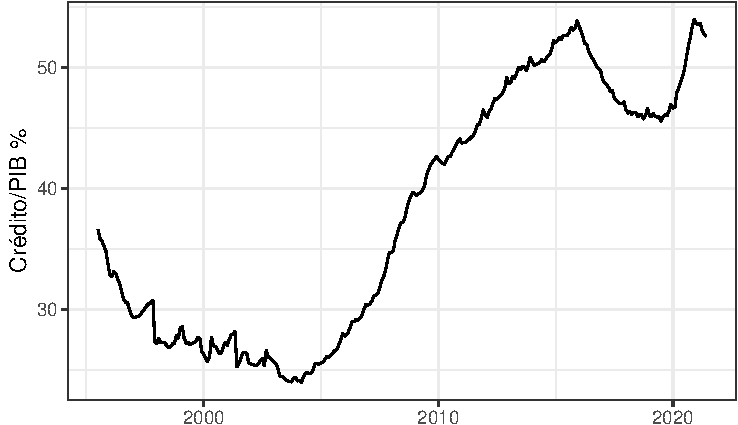
\includegraphics{12-exportedfigures/credit.gdp-1} \end{center}
\vspace{-3mm}
\label{graf:credgdp}
\fonte{Desenvolvido pelo autor, com dados o Banco Central}
\vspace{-2mm}
\end{grafico}

O \autoref{graf:credgdp} demonstra o comportamento da relação crédito/PIB no Brasil, que entre a segunda metade da década de 1990 até a meados da primeira metade da década de 2000 sofreu significativa queda, ficando abaixo dos 25\%. Após esse período a oferta de crédito ocorreu uma expansão exponencial atingindo um pico de 54.29\% do PIB.

Durante o período citado, foi observado no setor bancário brasileiro os maiores níveis de \emph{spread} praticados no mundo, associado a um quadro econômico instabilidades e baixos crescimento e desenvolvimento. Esse cenário encontra embasamento em estudos teóricos e empíricos que demonstram que um sistema financeiro desenvolvido favorece o crescimento e desenvolvimento econômico \cite{levine:1997, matos:2003}.

\begin{grafico}[!ht]
\vspace{20pt}
\caption{Evolução anual do saldo carteira de crédito}
\vspace{-4mm}

\begin{center}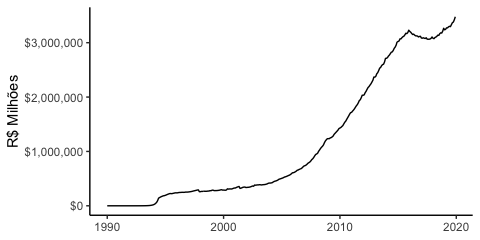
\includegraphics{12-exportedfigures/balance.credit-1} \end{center}
\vspace{-3mm}
\label{graf:saldocredito}
\fonte{Elaborado com dados do Banco Central}
\vspace{-2mm}
\end{grafico}

O \autoref{graf:saldocredito} demonstra a evolução do saldo da carteira de crédito de crédito livre e direcionado mensal em termos correntes, entre 1990 e 2020, podendo ser visualizada uma expansão exponencial de crédito a partir da metade da década de 2000, com leve recuo iniciado na metade da década de 2010, e posteriormente ultrapassando máxima anterior.

\subsection{Aspectos Monetários}

O Sistema Financeiro em sua organização entre agentes normatizadores, supervisores, operadores e tomadores, além suas instâncias, possui um papel fundamental na determinação de políticas para definição dos níveis adequados de base monetária e meios de pagamentos capazes de atender a atividade econômica, oferecendo liquidez e estabilidade .

Em consonância com o Conselho Monetário Nacional o Banco Central do Brasil tem como suas principais atribuições, a condução das políticas monetária, cambial e de crédito. Onde a oferta de crédito é influenciada pela políticas monetárias envolvendo e emissão de papel-moeda, taxa de compulsório, emissão de títulos públicos, entre outros, refletindo na base monetária e nos meios e pagamentos.

O multiplicador bancário, obtido da relação entre a oferta de crédito e a base monetária vem ser tornando cada vez mais relevante no processo de criação e destruição de moeda \cite{bacen:juros:1999, rey:2017, almonacid:1976}. Nesse sentido a base monetária se apresenta como elemento importante na determinação no nível de \emph{spread}, uma vez que se caracteriza como insumo para as operações de crédito.

A abordagem da base monetária como insumo para operações de crédito vem corroborar com a perspectiva do \cite{bacen:juros:1999}, do \emph{spread} como diferença entre a composição de custos entre as taxas de aplicação e taxa de captação, denotando assim o caráter de precificação ao \emph{spread}.

A Base Monetária restrita (\(M_0 = BMr\)) consiste no total de papel moeda emitido (\(PME\)) e das Reservas Bancárias (\(RB\)) em poder das instituições ou depositadas no Banco Central. Os dados são extraídos de contas analíticas no balanço do BACEN, consistindo na emissão primária de moeda e configurando o passivo monetário, resultado líquido de suas operações ativas e passivas \cite{bcb:2019}.

\begin{equation}
BMr = M_0 = PME + RB
\end{equation}

Em 1995 foi introduzido o conceito de Base Monetária ampliada (\(BMa = M_0\)), que possui maior capacidade de explanar os preços da economia no Brasil, uma vez que traz maior percepção do fator substituição entre a moeda, em seu conceito convencional, e os demais ativos financeiros disponíveis, incluindo os passivos, como os depósitos compulsórios (\(DC\)) e títulos públicos federais (\(TPF\)) \cite{bcb:2019}.

\begin{equation}
BMa = M_0 = BMr + DC +  TPF
\end{equation}

O \autoref{graf:moneybases} demonstra a evolução das bases monetárias restrita e ampliada, em termos correntes, entre os anos de 1995 e 2020. No início do período avaliado as séries estavam em patamares aproximados, ocorrendo um distanciamento exponencial ainda durante a década de 1990 e se tornando massivamente expressiva até o final do período.

\begin{grafico}[!htbp]
\vspace{20pt}
\caption{Evolução das bases monetárias restrita e ampliada — 1995 a 2020}
\vspace{-4mm}

\begin{center}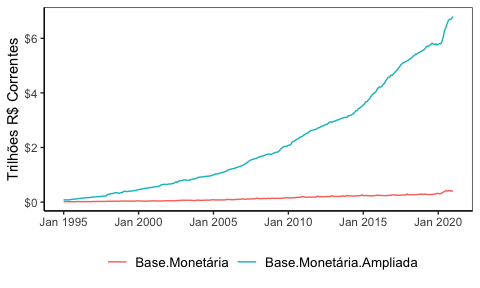
\includegraphics{12-exportedfigures/money.base.d-1} \end{center}
\vspace{-3mm}
\label{graf:moneybases}
\fonte{Desenvolvido com dados do Departamento de Estatísticas do Banco Central}
\vspace{-2mm}
\end{grafico}

O \autoref{graf:evpperb} demonstra a evolução do saldo de emissão de papel moeda e das reservas bancárias em termos correntes, entre 1995 e 2020, componentes da base monetária restrita. É possível observar que houve expressiva expansão do papel moeda emitido em termos correntes, e mesmo com elevação das reservas bancárias, houve uma desconexão entre as variáveis.

\begin{grafico}[!htbp]
\vspace{20pt}
\caption{Evolução da emissão de Papel Moeda e Reservas Bancárias}
\vspace{-4mm}

\begin{center}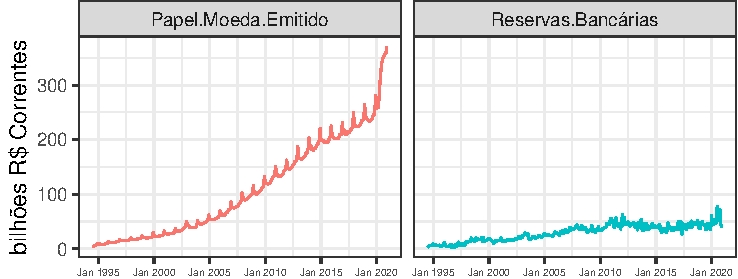
\includegraphics{12-exportedfigures/base.moneybase.e-1} \end{center}
\vspace{-3mm}
\label{graf:evpperb}
\fonte{Desenvolvido com dados do Departamento de Estatísticas do Banco Central}
\vspace{-2mm}
\end{grafico}

O \autoref{graf:evcomptit} traz a visualização das variáveis de Depósitos compulsórios e emissão de títulos públicos, sendo os componentes adicionais da base monetária ampliada que a diferencia da base monetária restrita. E mostra a larga expansão de emissão de títulos públicos totais, o que vem essencialmente explicar a diferenciação entre as séries de base monetária.

\begin{grafico}[!htbp]
\vspace{20pt}
\caption{Evolução dos Depósitos Compulsórios e emissão de títulos públicos}
\vspace{-4mm}

\begin{center}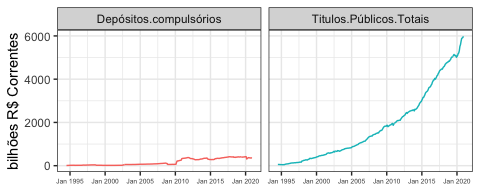
\includegraphics{12-exportedfigures/base.components-1} \end{center}
\vspace{-3mm}
\label{graf:evcomptit}
\fonte{Desenvolvido com dados do Departamento de Estatísticas do Banco Central}
\vspace{-2mm}
\end{grafico}

Entre os Agregados Monetários estão o Meios de Pagamento na forma restrita (\(M_1\)), configurado por cédulas e moedas em poder do público (\(PMPP\)) e seus depósitos a vista (\(DAV\)), disponíveis prontamente para pagamentos de bens e serviços. O conceito de Meios de Pagamentos Ampliado adiciona à moeda legal os agregados considerados de elevada liquidez (\(M_2\)) e (\(M_3\)) \cite{bcb:2019, sgs:mpa}.

\begin{equation}
M_1 = PMPP + DAV
\end{equation}

O Papel-moeda em poder do público (\(PMPP\)) é encontrado pelo resultado do papel moeda emitido (\(PME\)) subtraído dos encaixes do sistema bancário, obtidos diariamente em conta específica do balanço analítico Banco Central. Os depósitos a vista são aqueles remetem às captações pelos bancos criadores de moeda e transacionáveis por cheques ou meios eletrônicos \cite{sgs:m1}.

Os meios de pagamentos \(M_1\) consistem no passivo monetário de liquidez imediata do Banco Central e de instituições com poder emissão de moeda escritural e cooperativas de crédito, sendo registrados por regime de competência e gerados por estas instituições através do COSIF\footnote{ Realizados por meio de dados das demonstrações contábeis padronizadas}, SISBACEN\footnote{Dados de relatórios extracontábeis} e por instituições emissoras instrumentos monetários \cite{sgs:m1, sgs:mpa}.

O \autoref{graf:m1} traz a visualização da evolução dos saldos mensais de papel moeda em poder do público e dos depósitos a vista entre 1995 e 2020, em termos correntes. Nota-se que, até o ano de 2015, os depósitos a vista superavam o papel moeda em poder do público, quando essa relação se inverteu até meados de 2019 e passou a apresentar comportamento de igualdade até o início de 2020.

\begin{grafico}[!hbtp]
\vspace{20pt}
\caption{Evolução dos componentes que formam os Meios de pagamentos restritos M1 — 1995 à 2020}
\vspace{-4mm}

\begin{center}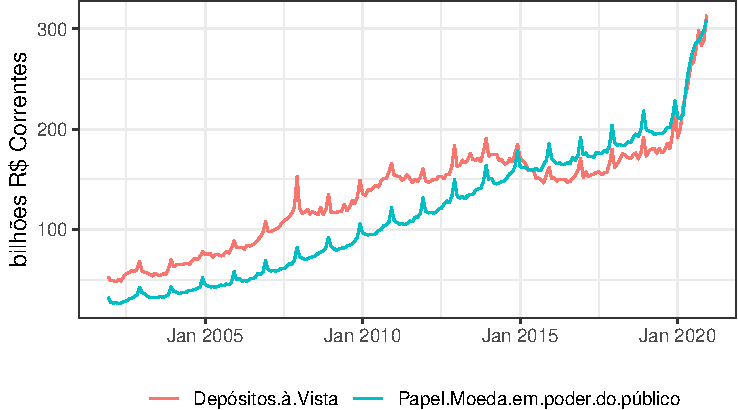
\includegraphics{12-exportedfigures/m1-1} \end{center}
\vspace{-3mm}
\label{graf:m1}
\fonte{Desenvolvido com dados do Departamento de Estatísticas do Banco Central}
\vspace{-2mm}
\end{grafico}

O Meios de Pagamentos Ampliados \(MPa\) consistem no conjunto de instrumentos monetários que remetem de forma antecipada à demanda por moeda, configurando uma avaliação do grau de liquidez da economia de uma forma mais precisa. Os meios de pagamentos amplos são formados pelos agregados monetários \(M_1\), \(M_2\), \(M_3\) e \(M_4\) \cite{sgs:mpa}.

No Brasil, a apuração e divulgação dos agregados monetários seguem as normas internacionais instituídas no Manual de Estatísticas Monetárias e Financeiras (MEMF), elaborado pelo Fundo Monetário Internacional (FMI) com a colaboração dos países participantes \cite{sgs:mpa}, o que vem trazer grandes vantagens técnicas para os países que aderem a estas normas.

O Agregado Monetário \(M_2\), contempla o Agregado Monetário \(M_1\) mais o resultante das emissões primárias por instituições depositárias no mercado interno, que realizam a multiplicação de crédito, consistindo em depósitos de poupança (\(DP\)) e títulos privados emitidos pelas instituições depositárias (\(TEID\))\footnote{Os títulos privados são compostos por Depósitos a prazo; Letras financeiras (LF); Letras de crédito do agronegócio (LCA); Letras de crédito imobiliárias (LCI); entre outros como aceites de letras de câmbio, Letras hipotecárias, Letras imobiliárias e Certificados de operações estruturadas} \cite{sgs:mpa}.

\begin{equation}
M_2 = M_1 + DP + TEID
\end{equation}

O Agregado Monetário \(M_3\) contempla o Agregado Monetário (\(M_2\)) adicionado das captações internas intermediadas pelos posição líquida de detentores moeda de renda fixa e das carteiras de títulos públicos federais registrados no Sistema Especial de liquidação e Custodia (Selic) e Bolsa de Valores. Consiste em quotas de fundos de renda fixa (\(QFRF\))\footnote{São considerados somente os fundos cambiais, renda fixa  e multimercado. excluídos os fundos de ações, fundos de dívida externa e os fundos de investimentos em quotas de fundos de investimentos , por serem considerados agentes não depositários, que não produzem liquidez ao mercado \cite{sgs:mpa}} e operações compromissadas registradas no Selic\footnote{As que são lastreadas em títulos públicos federais} (\(OCRS\)) \cite{bcb:2019} \cite{sgs:mpa}.

\begin{equation}
M_3 = M_2 + QFRF + OCRS
\end{equation}

O Agregado Monetário \(M_4\), que recebe o conceito de poupança financeira, contempla o Agregado Monetário \(M_3\) mais a carteira livre de títulos públicos federais\footnote{Consistindo somente os que estão devidamente registrados no Sistema Especial de Liquidação e Custódia (Selic), mesmo com elevada liquidez, há consenso que a classificação de quase-moeda deve ser restrita por não se configurar em uma instituição componente do Sistema Financeiro} de elevada liquidez (\(TPF\)) \cite{bcb:2019}.

\begin{equation}
M_4 = M_3 + TPF
\end{equation}

É possível chegar ao conceito de Agregado Monetário \(M_5\) que engloba o Agregado Monetário \(M_4\) incluindo a capacidade disponível de aquisição de cartões de crédito ativos (\(CACC\)) \cite{cordoba:1996}.

\begin{equation}
M_5 = M_4 + CACC
\end{equation}

O \autoref{graf:agrag} demonstra a evolução dos agregados monetários \(M_1\), \(M_2\), \(M_3\) e \(M_4\) em termos correntes, entre 2001 e 2020. É notado que os meios de pagamentos restritos \(M1\) sofreram expansão irrisória. Nos meios de pagamentos ampliados, no \(M_2\) é percebida uma considerável elevação, no \(M_3\) e \(M_4\) a expansão seguiu níveis exponenciais até o final do período.

\begin{grafico}[!hbtp]
\vspace{20pt}
\caption{Evolução dos Agregados monetários — 2001 à 2020}
\vspace{-4mm}

\begin{center}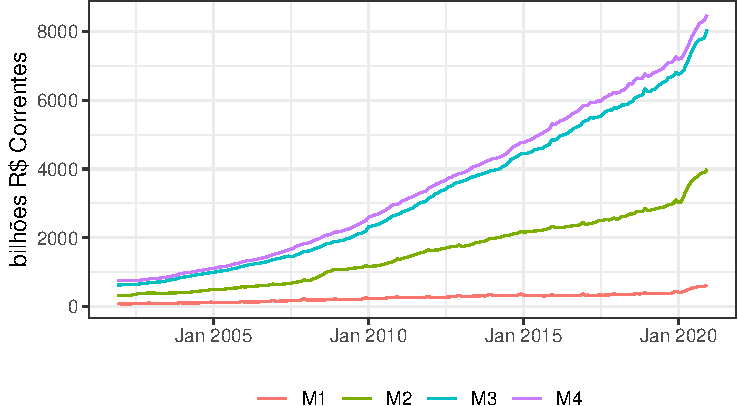
\includegraphics{12-exportedfigures/m2m3m4-1} \end{center}
\vspace{-3mm}
\label{graf:agrag}
\fonte{Desenvolvido com dados do Departamento de Estatísticas do Banco Central}
\vspace{-2mm}
\end{grafico}

De acordo com \textcite{friedman:1982}, o estudo do comportamento da demanda por moeda se relacionada intrisecamente com o estudo da velocidade da moeda. Em \textcite{friedman:1963} é abordado que a velocidade da moeda é determinada essencialmente pelo rendimento dos substitutos monetários, expectativas sobre a inflação e sensação sobre a estabilidade da economia.

A teoria quantitativa da moeda, prega que o nível de preços (\(P\)) em uma economia guarda relação com a quantidade de moeda em circulação (\(M\)) e a velocidade (\(V\)) de circulação --- frequência média em que uma unidade monetária é consumida em um período de tempo ---, diante seu produto real (\(y\)), com a premissa que no curto prazo o produto e a velocidade a moeda são constantes \cite{vasconcellos:2011, vieira:2016}.

\begin{equation}
MV = Py <=> P = \frac{MV}{y} <=> V = \frac{Py}{M}
\end{equation}

Neste contexto, uma vez que estudos sobre a velocidade da moeda guardam relação com estudos do comportamento da demanda por moeda, e consequentemente por crédito, tal variável se demonstra importante no estudos que visem avaliar os determinantes do \emph{spread} e da rentabilidade bancária.

De acordo com \textcite{bordo:1997} e \textcite{hafer:1991} para o caso americano o agregado monetário mais adequado para cálculo da velocidade da moeda é M2. Segundo \textcite{miller:1991} estudos que utilizam o M1 passa a ser duvidosos, pois de acordo com \textcite{baba:1992} o M1 não engloba as inovações financeiras, o que faz que estudos que utilizem apresentem instabilidade na demanda por moeda.

\subsection{Indicadores microeconômicos}

No que tange a abordagem microeconômica, as instituições bancárias como sociedade anônimas e instituições supervisionadas pelo Banco Central, são obrigadas a divulgar seus resultados em forma de demonstrações contábeis. A partir destas demostrações podem ser observados e extraídos dados e indicadores generalizados sobre a operação das instituições.

Os dados e estatísticas do Sistema Financeiro Nacional são compilados e divulgados pelo Banco Central com a legislação vigente, essencialmente seguindo a Lei nº 4.595, de 31 de dezembro de 1964 e Resoluções do Conselho Monetário Nacional, garantindo o sigilo de dados relativos às instituições financeiras, empresas e indivíduos\footnote{conforme disposto no artigo 2 da Lei Complementar nº 105, de 11 de janeiro de 2001} \cite{sgs:bm}.

A \autoref{tab:tabledocs} traz o resumo dos documentos que constituem as demonstrações contábeis padronizadas, enviadas pelas próprias instituições financeiras através do Sistema Contábil das Instituições Financeiras (COSIF), seguindo um conjunto de normas contábeis e plano de contas padronizados para os períodos definidos.

\begin{qdr}
\vspace{20pt}
\caption{Resumo das Demonstrações Contábeis Padronizadas}
\vspace{1mm}
\begingroup\fontsize{10}{12}\selectfont

\begin{tabu} to \linewidth {>{\raggedright}X>{\raggedright}X>{\raggedright}X>{\raggedright}X}
\toprule
Documento & Tipo & Códigos & Periodicidade\\
\midrule
\cellcolor{gray!6}{Balancete} & \cellcolor{gray!6}{Analítico} & \cellcolor{gray!6}{4010, 4020, 4413, 4433} & \cellcolor{gray!6}{Mensal ou Trimestral}\\
Balancete & Analítico Consolidado & 4040 & Mensal ou Trimestral\\
\cellcolor{gray!6}{Balancete} & \cellcolor{gray!6}{Analítico - Conglomerado Prudencial} & \cellcolor{gray!6}{4060} & \cellcolor{gray!6}{Mensal ou Trimestral}\\
Balanço & Analítico & 4016, 4026 & Semestral\\
\cellcolor{gray!6}{Balanço} & \cellcolor{gray!6}{Analítico Consolidado} & \cellcolor{gray!6}{4046} & \cellcolor{gray!6}{Semestral}\\
\addlinespace
Balanço & Analítico - Conglomerado Prudencial & 4066 & Semestral\\
\bottomrule
\end{tabu}
\endgroup{}
\vspace{1mm}
\label{tab:tabledocs}
\fonte{Desenvolvido a partir das fontes citadas}
\vspace{-2mm}
\end{qdr}

Os dados são divulgados seguindo uma padronização para o setor, onde podem ser observados as receitas, despesas, ativos, passivos, patrimônio líquido, entre outros em múltiplos níveis, para cada período de registo, buscando refletir a situação econômica e financeira, possibilitando a realização de análises evolutivas e comparativas e agregadas do setor financeiro.

Com acesso aos resultados contábeis é possível obter os principais indicadores para avaliação de resultados das instituições bancárias, como os índices de liquidez geral e liquidez corrente, endividamento e composição do endividamento, retorno sobre o ativo, retorno sobre o patrimônio líquido, margem EBITDA, margem líquida e grau de alavancagem financeira.

O índice de Liquidez Corrente (\(LC\)) mede a capacidade da instituição em honrar os compromissos com credores, definindo seu nível de solvência no curto prazo. É obtido pela razão entre o ativo circulante (\(AC\)) e o passivo circulante (\(PC\)), indicando o quanto do ativo circulante está disponível para cumprir com cada unidade monetária da dívida de curto prazo \cite{graham:2012} \cite{assaf:2020}.

\begin{equation}
LC = \frac{AC}{PC}
\end{equation}

O índice de Liquidez Geral (\(LG\)) mede a capacidade da instituição honrar os compromissos com seus credores no longo prazo, definindo seu nível de solvência geral, é obtido pela razão entre a soma do ativo circulante (\(AC\)) e recursos realizáveis no longo prazo (\(RLP\)) e a soma do passivo circulante (\(PC\)) e exigível no longo prazo (\(ELP\)) \cite{assaf:2020}.

\begin{equation}
LG_ = \frac{AC + RLP}{PC + ELP}
\end{equation}

O índice de endividamento (\(CT\)), mede a participação de capital de terceiros em relação aos financiamentos realizados com capital próprio. Quanto maior o indicador, maior a dependência da instituição de capital de terceiros para financiamento das suas operações, obtido pela razão entre o passivo (\(P\)) e o patrimônio líquido (\(PL\)) \cite{assaf:2020}.

\begin{equation}
CT = [\frac{P}{PL}]
\end{equation}

A composição do endividamento (\(CE\)) indica o percentual da dívida em relação a dívida que vence no curto prazo. Quanto maior for esse indicador, mais crítica é a situação, necessitando de melhores resultados para cumprir os compromissos no curto prazo. É obtido pela razão entre o passivo circulante (\(PC\)) e a soma do passivo circulante e exigível a longo prazo (\(ELP\)) \cite{assaf:2020}.

\begin{equation}
CE = \frac{PC}{PC + ELP}
\end{equation}

O Índice de Eficiência bancária (\(IE\)) avalia o quanto a instituição desembolsa para gerar uma unidade de receita. É obtido por meio da razão entre a soma das despesas administrativas (\(DA\)), despesas com pessoal (\(DP\)) líquidas da participação nos lucros (\(PLR\)) sobre a soma entre Margem Financeira (\(MF\)) e receita (\(R\)) \cite{timotio:2018}.

\begin{equation}
IE = \frac{DA + DP - PLR}{MF + R} 
\end{equation}

Outro indicador utilizado para avaliação da situação financeira das instituições bancárias é o obtido da relação entre as receitas de prestação de serviços (\(RSrv\)) e as despesas administrativas (\(DAdm\)) \cite{dantas:2012}.

\begin{equation}
RSDA = \frac{RSrv_{}}{DAdm{}}
\end{equation}

O retorno sobre o Ativo (\(ROA\)), mede a rentabilidade da instituição diante a totalidade dos seus ativos. O quanto para cada unidade monetária investida na instituição é convertida em lucro líquido, obtida da relação entre o lucro operacional (\(LO\)) e o ativo total (\(AT\)) \cite{assaf:2020}.

\begin{equation}
ROA = \frac{LO}{AT}
\end{equation}

O Retorno sobre o Patrimônio Liquido (\(ROE\)) mensura a relação entre o lucro líquido (\(LL\)) em o Patrimônio Líquido (\(PL\)) da instituição, configurando o retorno dos investimentos para os sócios e acionista, para cada unidade monetária com recursos próprios aplicados na empresa \cite{assaf:2020}.

\begin{equation}
ROE = \frac{LL}{PL}
\end{equation}

A margem EBITDA (\(MEB\)) é obtida da relação entre o EBITDA --- lucro antes dos juros, depreciação, amortização e impostos sobre a renda, configurando o lucro operacional da instituição --- e a Receita Líquida (\(RL\)), revelando a capacidade da instituição na geração de caixa \cite{assaf:2020}.

\begin{equation}
MEB_it = \frac{EBITDA_{it}}{RL_{it}}
\end{equation}

A Margem Líquida (\(ML\)) é um indicador que demonstra a parte de cada unidade monetária das intermediações financeiras que foi convertida em Lucro Líquido, sendo obtida da relação entre o lucro líquido (\(LL\)) e o resultado líquido da intermediação financeira (\(RLIF\)) \cite{assaf:2020}.

\begin{equation}
ML = \frac{LL}{RLIF}
\end{equation}

O grau de alavancagem financeira (\(GAF\)) captura o efeito da tomada de recursos de terceiros a um dado custo, alocados para ativos com distintas taxas de retornos. E mostra como se dá o aumento do lucro líquido através da estrutura de financiamento, definindo a parcela do retorno melhor ou pior se estivessem financiando a operações totalmente com capital próprio \cite{assaf:2020}.

\begin{equation}
GAF = \frac{RPL}{ROA}
\end{equation}

O risco de crédito das instituições bancárias pode ser obtido por meio da relação entre o saldo da Provisão para Créditos de Liquidação Duvidosa (\(PCLD\)) e do total da carteira de crédito (\(OPCR\)), obtidos através das contas 16900008 e 16000001 \cite{dantas:2012}

\begin{equation}
RC_{} = \frac{PCLD_{}}{OPCR_{}}
\end{equation}

A participação de mercado (\(MS\)) de cada instituição pode ser mensurada a partir da relação entre suas operações de crédito (\(OPCR\)) no total das operações de crédito do mercado, sendo obtido através da conta 1600001 \cite{dantas:2012}.

\begin{equation}
MS_{} = \frac{OPCR_{}}{\sum_{i}^{n}OPCR_{}} 
\end{equation}

Diante o levantamento, o setor bancário brasileiro durante o período avaliado passou por diversas transformações em sua estrutura no que tange a concentração de mercado, aumento da participação de capital estrangeiro por meio de controle acionário, redução da participação pública.

Em relação aos indicadores foi verificado que, entre a década de 1980 até metade da década de 1990, no cenário hiperinflacionário, mesmo com redução da concentração bancária, os indicadores de eficiência de intermediação financeiras como o \emph{spread} bancário e a relação crédito/PIB estavam em níveis considerados ineficientes e muito destoantes em comparação a outros países e regiões.

A partir de 1995 se observou mudanças significativas no setor bancário, com nova concentração, redução de instituições nacionais devido o controle acionário por capital estrangeiro, e expressiva redução no \emph{spread} bancário e a partir de 2004 uma mudança significativa no saldo da carteira de crédito e na relação crédito/PIB e na expansão das bases monetárias e meios de pagamentos ampliados.

Esta seção levantou informações amplas sobre o setor bancário brasileiro, identificando variáveis macroeconômicas e microeconômicas referentes a economia como um todo, setor financeiro, ao setor bancário e as instituições em si. No próximo capítulo serão levantados conceitos, definições e estudos sobre a evolução, decomposição e determinantes do \emph{spread} bancário.

\textual
\pagestyle{simple}
\parindent 1.50cm

\section{Spread Bancário}\label{sec:spread}

Esta seção irá tratar sobre os principais aspectos e características do \emph{spread} bancário. Na primeira parte serão abordados os conceitos e definições gerais. Na segunda parte as características amplas do mercado brasileiro. Na terceira parte sobre os estudos empíricos realizados no Brasil. O foco é identificar elementos que possam contribuir com o objeto deste estudo.

\begin{comment}
\textcolor{red}{DIFERENCIAR VARIÁVEIS IMPLÍCITAS E EXPLÍCITAS DO SPREAD}
\textcolor{red}{DIFERENCIAR VARIÁVEIS MICRO E MACRO}
\end{comment}

\subsection{Conceitos e Definições}

Por definição o termo \emph{spread} (\(Spr\)), que em tradução livre significa amplitude, crescimento e extensão, é utilizado no setor financeiro no sentido de margem, sendo obtido através da diferença entre a taxa de aplicação (\(TxApl\)) incidente nas operações de crédito e a taxa de captação (\(TxCap\)) que remunera as aplicações financeiras \cite{BCB:2000, BCB:1999}.

Em outra perspectiva, o \emph{spread} bancário implica na diferença entre a taxa de juros cobrada aos tomadores deficitários de recursos e a taxa básica de juros, referência para a remuneração das captações via depósitos, dos investidores superavitários de recursos financeiros, se configurando como a diferença entre a composição dos custos destas operações \cite{BCB:1999}.

\begin{equation}
Spr = TxApl - TxCap
\end{equation}

O \emph{spread} bancário representa uma medida que sinaliza o desempenho dos bancos \cite{levine:1997}. É considerado um indicador de eficiência da economia, influenciando o nível de crédito e a atividade econômica. Em níveis elevados pode desfavorecer o crédito destinado para produção e consumo produtivos e estar associado com baixo desenvolvimento econômico \cite{WB:2005}.

Os estudos em torno do \emph{spread} bancário ocorrem em três óticas: evolução, estrutura e determinantes \cite{dick:1999}. Em \textcite{dick:1999} é destacada a importância de distinguir as abordagens em torno da estrutura e determinantes do \emph{spread} bancário, porém no sentido de complementariedade. O diagrama na \autoref{fig:diagram.a} ilustra as óticas de estudo do \emph{spread} bancário.

\begin{figure}[!htbp]
\vspace{20pt}
\caption{Diagrama de ilustração da perspectiva de óticas de estudo do \emph{spread}}
\vspace{-4mm}

\begin{center}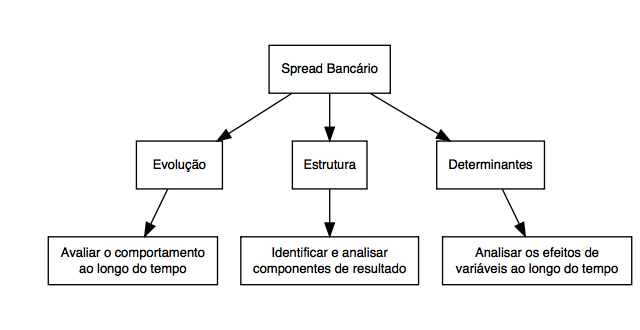
\includegraphics{12-exportedfigures/diagram.spread.otic-1} \end{center}
\vspace{-3mm}
\label{fig:diagram.a}
\fonte{Desenvolvido com base em \cite{dick:1999}}
\vspace{-2mm}
\end{figure}

A abordagem em torno da evolução visa analisar o comportamento ao longo do tempo, através de análises quantitativas e qualitativas. Enquanto a ótica da estrutura busca identificar e analisar os componentes de resultados envolvendo receitas, despesas e provisões. Na abordagem sobre os determinantes é vislumbrado identificar as variáveis que explicam as variações do indicador ao longo dos períodos \cite{dick:1999}.

Nas últimas décadas vem se tornando relevantes os estudos em torno da decomposição do \emph{spread} bancário (\(Sprd\)), em torno dos seus componentes. Entre os componentes explícitos estão a inadimplência (\(Ind\)), despesas administrativas (\(DAdm\)), impostos diretos (\(ImpDir\)) e indiretos (\(ImpInd\)), custos e despesas de captação (\(DesCap\)) e margem de lucro (\(MgLqd\)) dos bancos conforme ilustrado abaixo \cite{BCB:2000, BCB:1999}.

\begin{equation}
Sprd=f(Ind, DAdm, ImpInd, ImpDir, MgLqd, DesCap)
\end{equation}

Esta configuração contemplando a margem de lucro, despesas e riscos envolvidos nas operações de crédito vem desmistificar a comum abordagem do \emph{spread} como o rendimento auferido pelos bancos \cite{costa;nakane:2004, dantas:2012}. Desta forma implica na diferença entre o custos operacionais na ótica de precificação, que após descontados das receitas, remontam o lucro do banco \cite{BCB:2016}.

Além da avaliação de seus componentes, o \emph{spread} pode ser analisado
conjuntamente por três características: enquanto a abrangência da amostra,
conteúdo e origem da informação, conforme ilustrado na \autoref{fig:diagramb} \cite{leal:2006}. Estes três elementos estão interligados, podendo serem analisados separadamente ou em conjunto, trazendo vários níveis de informações.

\begin{figure}[!hbtp]
\vspace{20pt}
\caption{Diagrama de ilustração da perspectiva de características do \emph{spread}}
\vspace{-4mm}

\begin{center}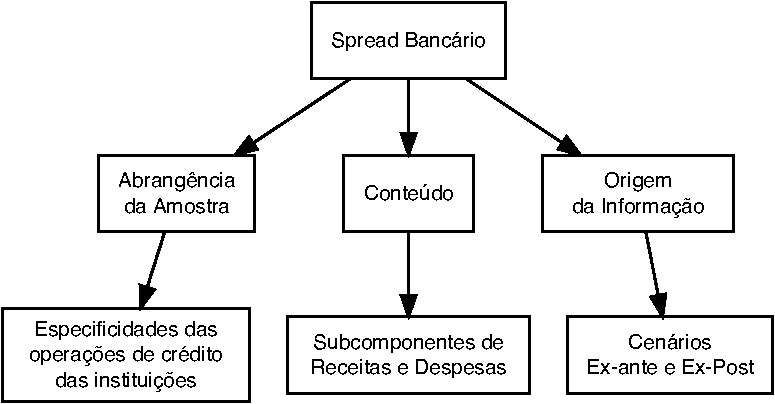
\includegraphics{12-exportedfigures/diagram.spread.carac-1} \end{center}
\vspace{-3mm}
\label{fig:diagramb}
\fonte{Desenvolvido com base em \cite{leal:2006}}
\vspace{-2mm}
\end{figure}

A abrangência da amostra consiste nas especificidades das operações de crédito das instituições e seu nível de agregação e granularidade \cite{costa;nakane:2004}. Uma análise agregada dessa característica pode ser dificultada pela existência de heterogeneidade do setor, ressaltando a importância de realizar análises do \emph{spread} bancário em diferentes características e óticas \cite{block:2000}.

A abordagem em torno do conteúdo está relacionada com os subcomponentes que envolvem a receita e as despesas das intermediações financeiras, podendo englobar, ou não, as tarifas e comissões sobre as taxas de captações e aplicação \cite{block:2000}. Porém com o formato atual dos dados divulgados, não é possível uma análises deste nível.

A origem da informação é analisada em dois cenários: \emph{ex-ante} e \emph{ex-post} \cite{kunt:1999, levine:1997}. A perspectiva \emph{ex-ante} refere-se ao planejamento e expectativas das instituições bancárias em relação ao mercado de crédito e os riscos envolvidos, obtido por método de precificação envolvendo as taxas de captação e empréstimo \cite{durigan:2018, leal:2006, dantas:2012}.

O \emph{spread} \emph{ex-ante}, por se tratar de um indicador de planejamento, refletindo as expectativas das instituições bancárias em relação ao mercado, finda demonstrando-se mais volátil, não representando as taxas efetivas realizadas. As informações \emph{ex-ante} são repassadas ao Banco Central que as divulga \cite{durigan:2018, leal:2006, dantas:2012}.

No \emph{spread ex-post} as margens são obtidas mediante a apuração dos resultados contábeis, através dos demonstrativos, considerando as receitas e custos efetivos, implicando nos resultados realizados pelas instituições financeiras \cite{kunt:1999, durigan:2018}. Nesse sentido, em termos médios, as taxas \emph{ex-post} se demonstram mais estáveis \cite{leal:2006, dantas:2012}.

Em oposição a medida de planejamento \emph{spread ex-ante}, disponibilizada de forma agregada, o \emph{spread ex-post}, por mostrar a diferença entre as taxas de aplicação e captação obtidas diretamente das demonstrações contábeis, se configura na efetiva margem realizada por cada instituições no período avaliado, e por isso com um maior para fins de análises \cite{dantas:2012}.

Como observado em \textcite{klein:1971} e \textcite{ho-saunders:1981} o \emph{spread} bancário é determinado de acordo com as características e os riscos envolvidos nas operações, inerentes em cada estrutura de mercado.Reduções no \emph{spread} \emph{ex-post} não necessariamente significam aumento da eficiência de intermediação, pois podem estar associadas a uma redução da inadimplência \cite{kunt:1999}.

\subsection{Spread Bancário no Brasil}

O Banco Central, em 1999, iniciou uma série de estudos e medidas com objetivo de reduzir a taxa de juros e o \emph{spread} realizados no setor bancário brasileiro, atuando na identificação e ajustes em variáveis econômicas influentes. Entre as primeiras medidas estavam a redução da taxa de compulsório para depósitos a vista e até a extinção para depósitos a prazo, redução do IOF e a redução da Selic \cite{BCB:2000}.

De acordo com o \textcite{BCB:1999}, adoção de política cambial de flutuação reduziram a necessidade de controlar o balanço de pagamentos através da imposição de elevadas taxas de juros básicas. Tais medidas combinadas com políticas de austeridade fiscal tiveram impactos positivos sobre a taxa de juros e sobre o \emph{spread} bancário.

No Brasil, a taxa de aplicação para crédito de recursos livres é pactuado entre instituição e tomador. Somente as operações de crédito envolvendo recursos direcionados são sujeitas à limites, não podendo exceder 12\% a.a. mais a taxa referencial de juros \cite{BCB:2016}.O que faz \emph{spread} bancário estar inserido nos mecanismos de mercado, sujeito a flutuações de oferta e demanda.

No mercado bancário brasileiro, o modelo consolidado de mensuração do \emph{spread} bancário, de acordo com demonstrado na \autoref{tab:spread.tb}, leva em consideração o saldo médio de capital emprestado, e a diferença entre as receitas de aplicação e despesas de captação, ocorrendo a classificação em \emph{spread} bruto, direto e líquido \cite{fipecafi:2005}

\begin{table}[!htbp]
\vspace{20pt}
 \centering
   \caption{Esquema de obtenção do \emph{Spread} mais adotado no mercado} 
   \vspace{1mm}
    \label{tab:spread.tb}
     \begin{tabular}{l|r|r|r}
      \hline
                                           &   PJ   &   PF    & Total \\
       \hline
       Saldo Médio do Capital Emprestado   & 100.00 & 100.00  & 100.00 \\
       A — Receita de Aplicação Financeira & 9.4    & 16.5    & 12,7   \\
       B — Despesas de Captação            & (4.8)  & (4.9)   & (4.8)  \\   
       Spread Bruto                        & 4.6    & 11.6    & 7.9    \\
       Spread Direto                       & 3.2    & 7.6     & 5.3    \\
       Spread Líquido                      & 0.5    & 1.6     & 1.0    \\
       \hline
       \end{tabular}
\vspace{1mm}
\fonte{in \cite{fipecafi:2005}}
\vspace{-2mm}
\end{table}

\begin{grafico}[!hbtp]
\vspace{20pt}
\caption{Evolução do \emph{spread} bancário brasileiro até 2011}
\vspace{-4mm}

\begin{center}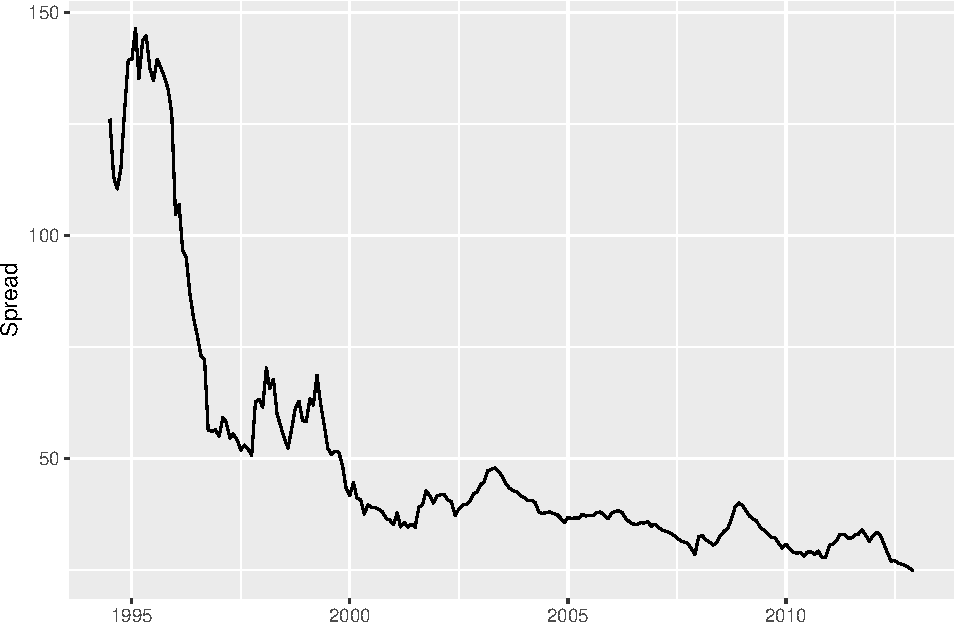
\includegraphics{12-exportedfigures/average spread-1} \end{center}
\vspace{-3mm}
\label{graf:spread2012}
\fonte{Desenvolvido a partir de dados do Banco Central}
\vspace{-2mm}
\end{grafico}

O \autoref{graf:spread2012} mostra a evolução do \emph{spread} bancário brasileiro médio entre os anos de 1994 e 2012, chegando a atingir 146.44\%, com significativa queda ao longo desse período, atingindo 24.69\% ao final. Esta série foi descontinuada em 2012, passando a ser utilizada nova metodologia de cálculo.

O Banco Central, até 2007 utilizava metodologia para avaliação do \emph{spread} bancário contemplando somente os recursos livres, o que não vinha a proporcionar uma avaliação mais aprofundada. Em 2008 houve uma modificação na metodologia de decomposição do \emph{spread}, alterando o cálculo do custo médio de captação e detalhando classificações do crédito \cite{dantas:2012}

Para o custo médio de captação passou a se utilizar a taxa média ponderada entre as taxas dos depósitos a prazo (CDB), caderneta de poupança e a vista, a participação dos custos efetivos dos recolhimentos compulsórios em detrimento do custo de oportunidade \cite{dantas:2012}

O BACEN mantém atualmente duas séries para o indicador: \emph{Spread} Médio das operações de crédito (MOC) e \emph{Spread} do Indicador de Custo de Crédito (ICC). As séries são disponibilizadas em termos totais e nas subdivisões por tipo de
recursos, crédito e tomador.

Estas séries estatísticas representam estimativas baseadas nas informações repassadas pelas instituições bancárias das taxas de juros das operações de crédito e indicadores do mercado financeiro do custo médio do dinheiro para o custo médio de captação \cite{BCB:2016}.

A série do \emph{Spread} médio das operações de crédito é calculada a partir da diferença entre a taxa média de juros de novas operações de crédito no SFN e o custo de captação referencial médio de operações de crédito livre, direcionado e não rotativo podendo ser observados por tomador \cite{BCB:2016}.

\begin{grafico}[!htbp]
\vspace{20pt}
\caption{Evolução do Spread médio das operações de crédito}
\vspace{-4mm}

\begin{center}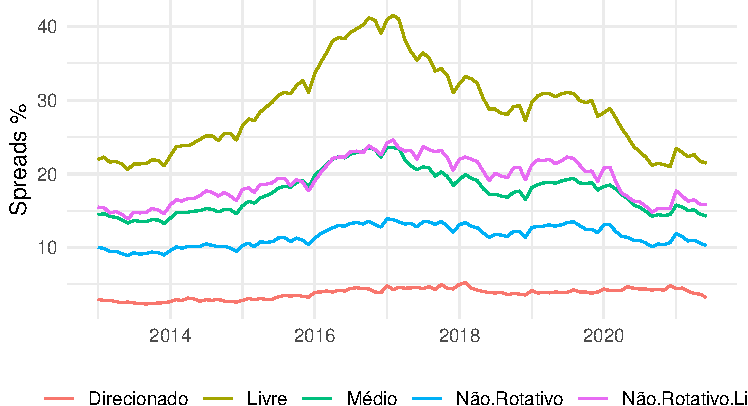
\includegraphics{12-exportedfigures/spread.2019.moc-1} \end{center}
\vspace{-3mm}
\label{graf:spreadmoc}
\fonte{Desenvolvido a partir de dados do Banco Central do Brasil — Departamento de Estatísticas}
\vspace{-2mm}
\end{grafico}

O \autoref{graf:spreadmoc} mostra a visualização da evolução mensal do spread médio das novas operações de crédito contratadas entre janeiro de 2013 e julho de 2020. No período entre 2014 e 2017 se verifica uma elevação de 10 p.p no \emph{spread} total, recuando 8 p.p a patamar próximo ao início do período. É possível notar a grande disparidade entre os \emph{spread} de recursos livres e direcionados.

O \emph{Spread} do ICC, considera a diferença entre o Índice de Custo de Crédito --- equivalente ao custo médio de juros das operações ativas da carteira do SFN --- e o custo de captação médio ponderado, levando em consideração operações de crédito livre, direcionado e não rotativo, subdividido por pessoa física e jurídica \cite{BCB:2016}.

\begin{grafico}[!htbp]
\vspace{20pt}
\caption{Evolução do \emph{Spread} do Índice do Custo de Crédito}
\vspace{-4mm}

\begin{center}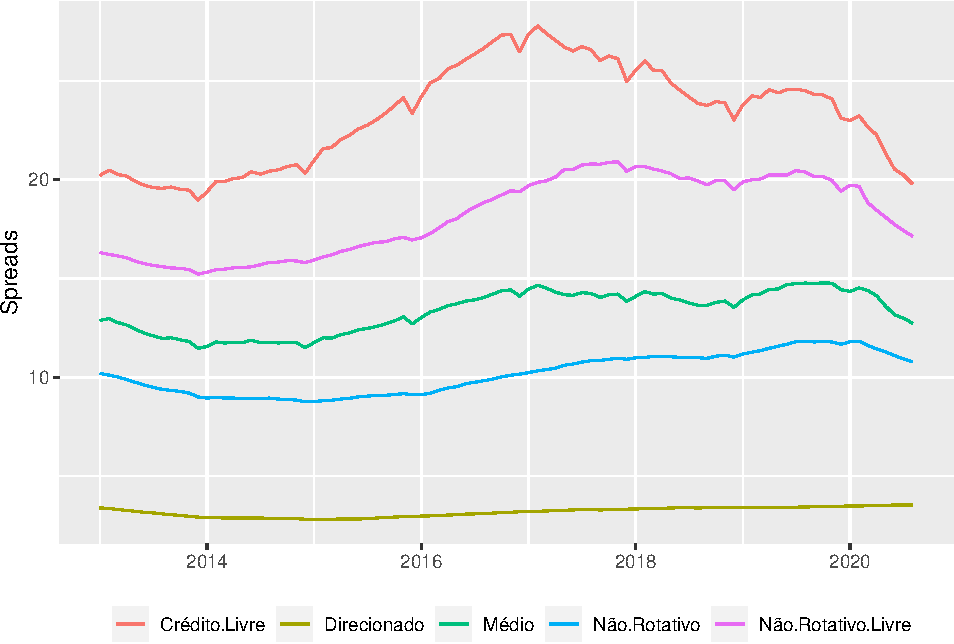
\includegraphics{12-exportedfigures/spread 2019 icc-1} \end{center}
\vspace{-3mm}
\label{graf:spreadicc}
\fonte{Desenvolvido a partir de dados do Banco Central do Brasil - Departamento de Estatísticas}
\vspace{-2mm}
\end{grafico}

No \autoref{graf:spreadicc} pode ser visualizada a evolução do \emph{spread} do ICC, entre janeiro de 2013 e julho de 2020 com expressiva elevação entre 2014 e 2017, passando a decair até retormar a patamares similares ao início do período. Também pode ser notada a expressiva diferença entre o \emph{spread} de recursos livres e direcionados.

Ao analisar as séries do \emph{Spread} ICC e \emph{Spread} MOC é possível destacar outra perspectiva de avaliação do \emph{Spread} no que tange a dimensão --- ilustrada na \autoref{fig:diagramc} ---, consistindo no tipo de recurso, modalidade e tomador, onde esta última aumenta o nível de granularidade abrangendo as demais. A perspectiva de dimensão atua de forma congruente com as perspectivas de ótica e de características.

O Indicador do Custo de Crédito (ICC) consiste no custo médio de todas as operações de crédito abertas --- independentes do período em que foram contratadas --- que compõem a carteira de empréstimos, financiamentos e arrendamento mercantil das instituições do Sistema Financeiro Nacional (SFN) \cite{BCB:2000}.

O \autoref{graf:evicc} traz a visualização da evolução do Índice de Custo de Crédito entre janeiro de 2013 e dezembro de 2020, com máxima de 22.98\% em 2017, demonstrando queda significativa a partir de 2020, chegando a atingir 16.76\% em agosto de 2020.

\begin{grafico}[!hbtp]
\vspace{20pt}
\caption{Evolução do Indicador de Custo de Crédito (ICC)}
\vspace{-4mm}

\begin{center}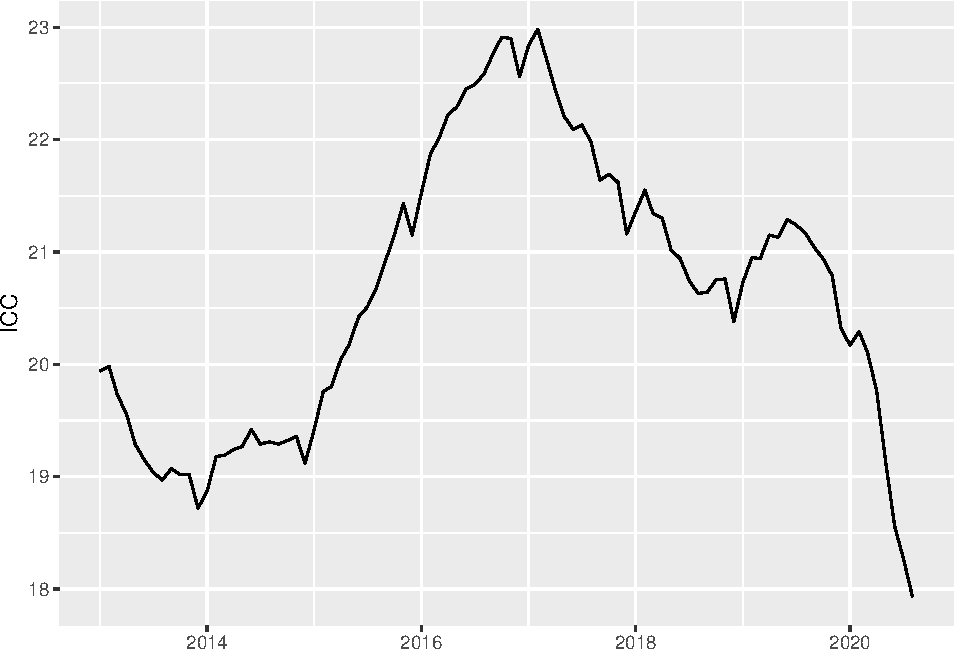
\includegraphics{12-exportedfigures/ICC-1} \end{center}
\vspace{-3mm}
\label{graf:evicc}
\fonte{Desenvolvido a partir de dados do Banco Central do Brasil — Departamento de Estatísticas}
\vspace{-2mm}
\end{grafico}

\begin{figure}[!htbp]
\vspace{20pt}
\caption{Diagrama de ilustração da perspectiva de dimensão  \emph{spread}}
\vspace{-4mm}

\begin{center}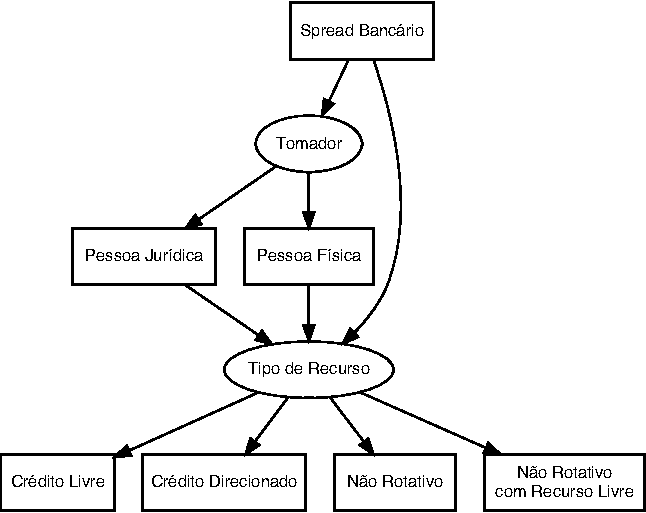
\includegraphics{12-exportedfigures/diagram.spread.dim-1} \end{center}
\vspace{-3mm}
\label{fig:diagramc}
\fonte{Desenvolvido com base nos dados}
\vspace{-2mm}
\end{figure}

A perspectiva de dimensão demonstra ser relevante, uma vez que existem diferenças consideráveis para os níveis de \emph{spread} de acordo com tomador, tipo de crédito e modalidade. Levantando a indagação se uma análise agregada é capaz identificar de forma realística os efeitos desta variáveis sobre os setores produtivos.

Em \textcite{BCB:1999} é abordado sobre a diversidade das operações de crédito que envolvem o volume, prazos, garantias, tipo de recursos e tomadores. Tal abordagem vem corroborar com perspectiva de dimensão e levanta uma outra perspectiva no que tange o volume-prazo-risco, conforme ilustrado na \autoref{fig:diagramd}.

\begin{figure}[!htbp]
\vspace{20pt}
\caption{Diagrama de ilustração da perspectiva volume-tempo-risco  \emph{spread}}
\vspace{-4mm}

\begin{center}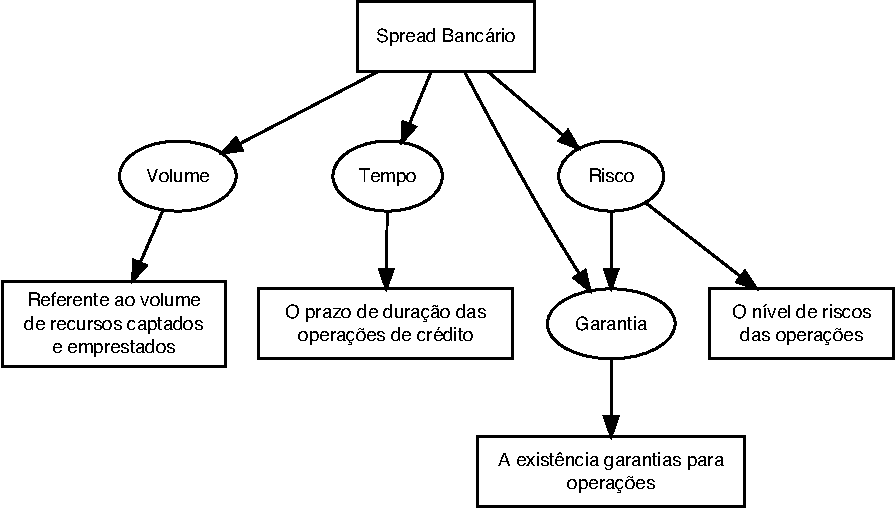
\includegraphics{12-exportedfigures/diagram.spread.vol.tem,ris-1} \end{center}
\vspace{-3mm}
\label{fig:diagramd}
\fonte{Desenvolvido com base nos dados}
\vspace{-2mm}
\end{figure}

\subsection{Estudos anteriores}

Na literatura acadêmica não existe uma teoria formalizada acerca do \emph{spread} bancário \cite{timotio:2018}. Sendo verificados estudos empíricos que visam classificar, analisar e identificar variáveis microeconômicas e macroeconômicas influentes nesse indicador em diversas perspectivas.

Em estudo, \textcite{BCB:1999}\footnote{Neste estudo foram desconsiderados dados de operações de repasses governamentais, crédito imobiliário, crédito rural e taxas estabelecidas} apresenta como composição do \emph{spread} a inadimplência, despesas administrativas impostos indiretos, imposto de renda, contribuição social do lucro líquido e a margem de lucro dos bancos e despesas de captação. Nos resultados o estudo concluiu que a taxa básica de juros explicam somente uma parte das juros e \emph{spread}.

Ainda em \textcite{BCB:1999}, é abordado a relação inversa entre a taxa básica de juros e spread com a demanda interna, atuando via a elevação da oferta de crédito, combinados com redução da taxa de compulsório e políticas de concessão de crédito. E que alterações na taxa básica de juros afetam toda a cadeira de taxas até consumidor final, em uma estrutura de custos das operações em degraus\footnote{Configurado por taxas preferenciais mais baixas e risco de crédito elevado}.

Outro aspecto levantado por \textcite{BCB:1999}, é que no período levantado, o \emph{spread} não demonstrou instabilidade diante a volatilidade da taxa básica de juros, que apresentou grande variação durante o período. Verificando que o custo de crédito em suas modalidades refletem as alterações na taxa básica de juros.

De acordo com \textcite{BCB:1999}, a inadimplência é o componente mais oneroso do \emph{spread}, representado 35\%. Os componentes de markup: impostos indiretos (14\%\footnote{Nesse cálculo está incluída a extinta CMPF}), despesa administrativas (22\%), IR e CSLL (11\%) e margem de lucro do bancos (18\%) são apresentado como relevantes e determinantes na explicação do spread.

Em \textcite{BCB:1999}, o risco de crédito foi apresentado como determinante, no custo da operação, por implicar na decisão de concessão, onerando as demais operações realizadas. Pois ao emprestar o capital de terceiros os bancos assumem o risco, e buscam minimizar com uma cobrança adicional associada a probabilidade de não receber, onde tal avaliação poder ser arbitrária.

O risco de crédito e inadimplência estão relacionados em parte com fatores definidos no ambiente macroeconômico e outra parte com as características institucionais individuais, no que tangem a capacidade de avaliação de crédito.
Segundo \textcite{BCB:1999} as despesas administrativas estão relacionadas com a eficiência, quantidade de agências e grau de alavancagem das operações de crédito. E quanto menor o volume da operações, maior será a participação das despesas administrativas, com tendência ser repassada ao tomador final.

No estudo, \textcite{BCB:1999} verificou que o repasse do juros ocorre mesmo com o utilização do capital próprio, incluindo a parcela de imposto de renda e contribuição social inerentes as operações de captação. E que os maiores níveis de spread são os de cheque especial, no qual não guarda relação risco, mas elevadas margens de lucros associada o poder de mercado das instituições.

Em \textcite{BCB:1999} foi verificado que o impactos dos impostos indiretos são mais elevados para as pessoas físicas do que para pessoas jurídica , principalmente por conta do IOF. O mesmo ocorre com as despesas administrativas, repasse de riscos e margem de lucro, que por conseguinte elevam o PIS e COFINS.

O comportamento social e cultura também são apontados como fatores determinantes, em \textcite{BCB:1999}, afetando a inadimplência na perspectiva de risco moral. E que o aspectos jurídicos em torno de cobrança acabam agravando a inadimplência. Sugerindo que as instituições financeiras deveriam ser vistas como parceiras no processo econômico.

Para \textcite{BCB:1999}, em grande parcela o \emph{spread} pode ser explicado pela inadimplência, e pelo reduzido nível de alavancagem financeira, reduzindo a dispersão dos custos administrativos e de capital nas operações de crédito. A inadimplência age limitando a carteira de crédito, mantendo a alavancagem baixa, como uma forma de proteção para as instituições.

Entre outros aspectos relevantes apontados em \textcite{BCB:1999}, estão a importância de um ambiente macroeconômico favorável, redução da cunha fiscal, controle da inflação, aumento da oferta de crédito, redução de compulsórios e créditos direcionados e redução das taxas básicas de juros.

A grande maioria dos estudos realizados no Brasil utilizam as medidas de
\emph{spread} bancário divulgadas pelo Banco Central, que remetem a uma perspectiva
\emph{ex-ante}, registrando as taxas planejadas na fase de concessão de crédito. E
para as variáveis explicativas a grande maioria utiliza indicadores
macroeconômicos \cite{dantas:2012}

No ano de 1994, \textcite{aronovich:1994} realizou estudo econométrico para
verificar a influência da inflação e nível de atividade econômica no \emph{spread}
bancário \emph{ex-ante}, encontrando relação direta do \emph{spread} com a inflação e
indireta com o nível de atividade econômica.

Em estudo dos determinantes macroeconômicos do \emph{spread} bancário \emph{ex-ante}, \textcite{oreiro-2006} utilizou modelo de regressão múltipla\footnote{$ln spread = \beta_0 trend + \beta_1 ln selic + \beta_2 ln adm + \beta_3 ln risk + \beta_4 ln imp + \beta_5 ln comp$}\footnote{trend = tendência determinista que controla outras variáveis; selic = taxa Selic; adm = despesa administrativas; risk =  proxy para o risco de crédito (spread do C-Bond sobre o rendimento dos títulos do Tesouro Americano de mesma maturidade; imp são impostos indiretos; comp = compulsório incidente sobre os depósitos a vista.} --- para identificar as variáveis influentes. O estudo chegou ao resultado que a alta volatilidade e as taxas da Selic são um dos principais determinantes desse indicador no setor bancário brasileiro, identificando também a significância do nível de atividade industrial.

Em análise dos determinantes do \emph{spread} bancário \emph{ex-post}, \textcite{dantas:2012} utilizou modelo de dados microeconômicos em painel dinâmico (jan-2000 a out-2009), encontrando níveis significativos e diretos com o risco de crédito, concentração, atividade econômica, e indireta com a participação de mercado, não encontrando níveis significativos com origem de capital e tipo de organismo.

Outra observação em \textcite{dantas:2012}, foi a forte relação do \emph{spread} \emph{ex-post} no momento atual com o momento anterior imediato, e que as instituições tendem a cobrar maiores taxas, quando maior o nível de concentração do mercado e não encontrou significância da Selic na determinação deste indicador.

Em \textcite{almeida:2013} foi desenvolvido modelo de dados macroeconômicos e microeconômicos em painel de 64 instituições bancárias para avaliação de determinantes do \emph{spread} \emph{ex-post} no Brasil entre o primeiro trimestre de 2001 e o segundo trimestre de 2012, encontrando como relevantes as despesas administrativas, receita de serviços, índice de cobertura, PIB e o grau de concentração.

Em \textcite{durigan:2018} foi realizada análise dos fatores macroeconômicos e indicadores industriais que influenciam o \emph{spread} bancário \emph{ex-ante}, através de análise de regressão linear multivariada utilizando 18 variáveis em quatro modelos. Chegando a conclusão que o aumento da atividade industrial, a redução
do desemprego e o consumo atuam na diminuição do \emph{spread} bancário.

Os modelos desenvolvidos por \textcite{durigan:2018} demonstraram que há uma relação significativa e direta entre \emph{spread} e: inadimplência, IPIs (bens de capital, intermediários, semiduráveis, não duráveis e consumo duráveis), Selic, PIB, desemprego e o EMBI+\footnote{Medida de taxa de risco-país}. As relações indiretas foram encontradas em: IPI (bens de consumo e geral), IPCA, saldo da carteira de crédito e índice de vendas no varejo.

O estudo de \textcite{timotio:2018} teve foco em abordagem microeconômica ao buscar identificar a influência das variações de indicadores financeiros-contábeis no \emph{spread ex-post} em 26 instituições bancárias, através de regressão em dados em painel. Encontrando relações significativas diretas com a alavancagem financeira, retorno sobre o patrimônio líquido, EBITDA, Ativo Total e eficiência.

No modelo de \textcite{timotio:2018} foi encontrada relação significativa e indireta do \emph{spread} com a participação de capital de terceiros e, não identificada relação significativa com a composição do endividamento, retorno sobre ativos e a liquidez corrente.

De acordo com \textcite{durigan:2018, dantas:2012}, existem poucos estudos inclinados para os determinantes do \emph{spread} \emph{ex-post} no Brasil, onde identificaram o estudos de Guimarães (2002). Foram identificados ainda os estudos acerca do \emph{spread} ex-post de Fipecafi (2004) \emph{apud} \textcite{dantas:2012} e Matias (2006) \emph{apud} \textcite{leal:2006}.

Em \textcite{fipecafi:2005} foi realizado estudo de apuração de resultados, \emph{ex-post}, baseado em demonstrações contábeis entre o 1º semestre de 2005 de instituições que representavam 75,8\% do ativo total e 76\% do total de crédito. Chegando a um resultado médio de \emph{spread} bruto de 7,6\% para pessoa física e 3,2\% para pessoa jurídica, e \emph{spread} líquido de 1,6\% para pessoa física e 0,5\% para pessoa jurídica.

O \autoref{qdr:exantea} e o \autoref{qdr:exanteb} trazem o resumo dos principais estudos empíricos sobre \emph{spread} bancário \emph{ex-ante} no Brasil, com resultados obtidos através de modelagem econométrica com utilização de regressão, tomando variáveis micro e macroeconômicas como explanatórias e demonstrando a relação com o \emph{spread ex-ante}.

\begin{qdr}
\vspace{20pt}
\caption{Resumo de estudos sobre o \emph{spread ex-ante} no Brasil — Parte 1}
\vspace{1mm}
\begingroup\fontsize{10}{12}\selectfont

\begin{tabu} to \linewidth {>{\raggedright\arraybackslash}p{4cm}>{\raggedright\arraybackslash}p{2cm}>{\raggedright\arraybackslash}p{2cm}>{\raggedright\arraybackslash}p{2cm}>{\raggedright\arraybackslash}p{2cm}}
\toprule
Variável & KOYAMA e NAKANE (2001a e 2001b) & AFANASIEFF, LHAGER e NAKANE (2001) & AFANASIEFF, LHAGER e NAKANE (2002) & BIGNOTTO e RODRIGUES (2006)\\
\midrule
\textbf{\cellcolor{gray!6}{Custos Administrativos}} & \cellcolor{gray!6}{+} & \cellcolor{gray!6}{+} & \cellcolor{gray!6}{+} & \cellcolor{gray!6}{+}\\
\textbf{IGP} & + & + & - & \\
\textbf{\cellcolor{gray!6}{Impostos Indiretos}} & \cellcolor{gray!6}{+} & \cellcolor{gray!6}{+} & \cellcolor{gray!6}{+} & \cellcolor{gray!6}{}\\
\textbf{Requerimento de Reserva} & + &  &  & \\
\textbf{\cellcolor{gray!6}{Selic}} & \cellcolor{gray!6}{+} & \cellcolor{gray!6}{+} & \cellcolor{gray!6}{+} & \cellcolor{gray!6}{+}\\
\addlinespace
\textbf{Spread Over Treasury} & + &  & + & \\
\textbf{\cellcolor{gray!6}{Produto Industrial}} & \cellcolor{gray!6}{-} & \cellcolor{gray!6}{} & \cellcolor{gray!6}{} & \cellcolor{gray!6}{}\\
\textbf{Ativo Total} &  &  &  & +\\
\textbf{\cellcolor{gray!6}{Bancos Estrangeiros}} & \cellcolor{gray!6}{} & \cellcolor{gray!6}{} & \cellcolor{gray!6}{-} & \cellcolor{gray!6}{}\\
\textbf{Captação sem juros} &  & + & + & \\
\addlinespace
\textbf{\cellcolor{gray!6}{Compulsório}} & \cellcolor{gray!6}{} & \cellcolor{gray!6}{} & \cellcolor{gray!6}{} & \cellcolor{gray!6}{+}\\
\textbf{Crescimento PIB Industrial} &  & - & + & \\
\textbf{\cellcolor{gray!6}{IPCA}} & \cellcolor{gray!6}{} & \cellcolor{gray!6}{} & \cellcolor{gray!6}{} & \cellcolor{gray!6}{-}\\
\textbf{Liquidez} &  &  &  & +\\
\textbf{\cellcolor{gray!6}{Market Share}} & \cellcolor{gray!6}{} & \cellcolor{gray!6}{} & \cellcolor{gray!6}{} & \cellcolor{gray!6}{-}\\
\addlinespace
\textbf{Receita Serviços} &  & + & + & +\\
\textbf{\cellcolor{gray!6}{Risco Crédito}} & \cellcolor{gray!6}{} & \cellcolor{gray!6}{} & \cellcolor{gray!6}{} & \cellcolor{gray!6}{+}\\
\textbf{Risco Juros} &  &  &  & +\\
\textbf{\cellcolor{gray!6}{Volatilidade da Selic}} & \cellcolor{gray!6}{} & \cellcolor{gray!6}{-} & \cellcolor{gray!6}{} & \cellcolor{gray!6}{}\\
\bottomrule
\end{tabu}
\endgroup{}
\vspace{1mm}
\label{qdr:exantea}
\fonte{Desenvolvido a partir das fontes citadas}
\vspace{-2mm}
\end{qdr}

Entre os estudos do \autoref{qdr:exantea} e \autoref{qdr:exanteb} que avaliaram a Selic e as despesas administrativas, há um consenso que estas variáveis possuem uma relação de determinação direta com o \emph{spread ex-ante}. Em três estudos que avaliaram impostos indiretos e receita de serviços foi encontrada relação direta com o \emph{spread ex-ante}.

\begin{qdr}
\vspace{20pt}
\caption{Resumo de estudos sobre o \emph{spread ex-ante} no Brasil — Parte 2}
\vspace{1mm}
\begingroup\fontsize{10}{12}\selectfont

\begin{tabu} to \linewidth {>{\raggedright\arraybackslash}p{4cm}>{\raggedright\arraybackslash}p{3cm}>{\raggedright\arraybackslash}p{3cm}>{\raggedright\arraybackslash}p{3cm}}
\toprule
Variável & OREIRO et al. (2006) & DURIGAN (2018) & ARONOVICH (1994)\\
\midrule
\cellcolor{gray!6}{Selic} & \cellcolor{gray!6}{+} & \cellcolor{gray!6}{+} & \cellcolor{gray!6}{}\\
Produto Industrial & + &  & \\
\cellcolor{gray!6}{Atividade Econômica} & \cellcolor{gray!6}{} & \cellcolor{gray!6}{} & \cellcolor{gray!6}{-}\\
Desemprego &  & + & \\
\cellcolor{gray!6}{EMBI} & \cellcolor{gray!6}{} & \cellcolor{gray!6}{+} & \cellcolor{gray!6}{}\\
\addlinespace
Inadimplência &  & + & \\
\cellcolor{gray!6}{Índice Volume Vendas Varejo} & \cellcolor{gray!6}{} & \cellcolor{gray!6}{-} & \cellcolor{gray!6}{}\\
IPCA &  & - & +\\
\cellcolor{gray!6}{IPI bcd} & \cellcolor{gray!6}{} & \cellcolor{gray!6}{+} & \cellcolor{gray!6}{}\\
IPI Bens de Capital &  & + & \\
\addlinespace
\cellcolor{gray!6}{IPI Bens de Consumo} & \cellcolor{gray!6}{} & \cellcolor{gray!6}{-} & \cellcolor{gray!6}{}\\
IPI Bens i &  & + & \\
\cellcolor{gray!6}{IPI bsd} & \cellcolor{gray!6}{} & \cellcolor{gray!6}{+} & \cellcolor{gray!6}{}\\
IPI Geral &  & - & \\
\cellcolor{gray!6}{IPIad} & \cellcolor{gray!6}{} & \cellcolor{gray!6}{+} & \cellcolor{gray!6}{}\\
\addlinespace
PIB &  & + & \\
\cellcolor{gray!6}{Saldo Carteira Crédito RL} & \cellcolor{gray!6}{} & \cellcolor{gray!6}{-} & \cellcolor{gray!6}{}\\
Volatilidade da Selic & + &  & \\
\bottomrule
\end{tabu}
\endgroup{}
\vspace{1mm}
\label{qdr:exanteb}
\fonte{Desenvolvido a partir das fontes citadas}
\vspace{-2mm}
\end{qdr}

Ainda no \autoref{qdr:exantea} e \autoref{qdr:exanteb}, dois estudos chegaram a resultados diferentes para a volatilidade da Selic. Os efeitos do IPCA foram testados em três estudos, os dois mais recentes encontraram uma relação indireta. Em três estudos que examinaram o IGP, dois encontram relação direta, um deles foi repetido posteriormente e encontrou relação indireta.

\begin{qdr}
\vspace{20pt}
\caption{Resumo de estudos sobre o \emph{spread ex-post} no Brasil}
\vspace{1mm}
\begingroup\fontsize{10}{12}\selectfont

\begin{tabu} to \linewidth {>{\raggedright\arraybackslash}p{4cm}>{\raggedright\arraybackslash}p{3cm}>{\raggedright\arraybackslash}p{3cm}>{\raggedright\arraybackslash}p{3cm}}
\toprule
Variável & GUIMARÃES (2002) & DANTAS (2012) & ALMEIDA (2013)\\
\midrule
\textbf{\cellcolor{gray!6}{Custos Administrativos}} & \cellcolor{gray!6}{} & \cellcolor{gray!6}{} & \cellcolor{gray!6}{+}\\
\textbf{Impostos Indiretos} &  &  & Não significativo\\
\textbf{\cellcolor{gray!6}{Requerimento de Reserva}} & \cellcolor{gray!6}{} & \cellcolor{gray!6}{} & \cellcolor{gray!6}{+}\\
\textbf{Atividade Econômica} &  & + & \\
\textbf{\cellcolor{gray!6}{Bancos Estrangeiros}} & \cellcolor{gray!6}{+} & \cellcolor{gray!6}{} & \cellcolor{gray!6}{}\\
\addlinespace
\textbf{Caixa.Depósitos} & + &  & \\
\textbf{\cellcolor{gray!6}{Grau Concentração}} & \cellcolor{gray!6}{} & \cellcolor{gray!6}{+} & \cellcolor{gray!6}{+}\\
\textbf{Liquidez} &  &  & Não significativo\\
\textbf{\cellcolor{gray!6}{Market Share}} & \cellcolor{gray!6}{} & \cellcolor{gray!6}{-} & \cellcolor{gray!6}{+}\\
\textbf{PIB} &  &  & +\\
\addlinespace
\textbf{\cellcolor{gray!6}{Receita Serviços}} & \cellcolor{gray!6}{} & \cellcolor{gray!6}{} & \cellcolor{gray!6}{-}\\
\textbf{Risco Crédito} &  & + & Não significativo\\
\bottomrule
\end{tabu}
\endgroup{}
\vspace{1mm}
\label{qdr:expost}
\fonte{Desenvolvido a partir das fontes citadas}
\vspace{-2mm}
\end{qdr}

O \autoref{qdr:expost} traz o resumo dos estudos empíricos dos determinantes do\emph{spread ex-post} no Brasil, por meio de modelos econométricos utilizando regressão. Destaca-se que, entre os estudos, dois encontraram significância de influência direta com o grau de concentração e o \emph{spread ex-post}. E dois dos estudos chegaram a resultados opostos para posição de market share e a variável dependente.

Este capítulo verificou os principais conceitos, características e estudos acerca do \emph{spread} bancário no Brasil, identificando as óticas de análise por evolução, composição e determinantes através da abrangência da amostra, conteúdo e origem da informação e por dimensão por tipo de empréstimo e tomador.

Ainda foi verificado que as maiores limitações estão na dificuldade de desagregação de informações para uma análise mais aprofundada, prejudicando as análises de determinantes do \emph{spread ex-post}. E a maioria dos estudos mais significativos estão relacionados ao \emph{spread ex-ante}.

No próximo capítulo, será descrita a metodologia de trabalho com a formulação das hipóteses baseado nas informações e levantamentos dos capítulos anteriores, nos estudos pesquisados e na teoria econômica, através da coleta, tratamento e análise de dados.

\textual
\pagestyle{simple}
\parindent 1.50cm

\chapter{Procedimentos Metodológicos}

Neste capítulo serão descritos os principais procedimentos metodológicos, técnicas e ferramentas que serão utilizados neste trabalho, visando organizar as etapas da pesquisa e permitir um maior nível de reproducibilidade, revisão e refutabilidade da mesma.

Este trabalho está sendo desenvolvido e editado em ambiente R Markdown com utilização de linguagem Latex para padronização de textos, figuras e tabelas, e as linguagens R e Python para coleta, limpeza, tratamento, análise, visualização, modelagem e estimação econométrica dos conjuntos de dados.

Na primeira parte serão apresentados concepções, pressupostos e critérios teóricos e técnicos diante o conjunto de informações e dados levantados, que servirão como pilar para a construção da modelagem econométrica. Na segunda parte serão trazidas as características teóricas da modelagem selecionada. E na última parte serão expostas as hipóteses com detalhamentos das variáveis.

Para fins de modelagem, o \emph{spread} será abordado dentro do conceito de precificação, seguindo a decomposição desenvolvida no \autoref{apendicea}, na forma simplificada da \autoref{eq:amor05} e dos componentes da taxa de juros conforme a \autoref{eq:txjur100}.

\begin{equation}\label{eq:amor100}
SprEp_{[n,a,b,c,d,e]} = \left[ \frac{ROp_{n}[\frac{   ijr_{}  }{  [1 + ijr_{}]^n -1  }]}{Op_{n}} -1 \right] - \left[ \frac{DC_{n}}{C_{n}} \right]
\end{equation}

\begin{equation}\label{eq:txjur100}
\begin{aligned}
ijr_{[t(a,b,c,d,e)]} = & \frac{[i_{adm} + i_{Inad} + i_{IOF} + r +  \frac{(i_{cap} + i_{fgc} + i_{ac}.i_{comp} - i_{r}.i_{fgc}+ i_{cs}.i_{fgc})}{1 - i_{comp} - i_{fgc}}]}
{[1 - (\frac{i_{ll}}{1 - i_{r} - i_{cs}} + i_{pis}.(1 - i_{r} - i_{cs}) + i_{cof}.(1 - i_{r} - i_{cs}) + 0,99i_{r} + i_{cs})]}v'p'g'
\end{aligned}
\end{equation}

\begin{comment}
\textcolor{red}{COMEÇAR APRESENTANDO O MODELO}
\textcolor{red}{DEFINIR POPULAÇÃO E DEFINIR PARCIAL - AMOSTRA}
\textcolor{red}{METODOLOGIA FRÁGIL}
\textcolor{red}{PADRONIZAR VARIÁVEIS}
\textcolor{red}{VERIFICAR AS LETRAS NAS EQUAÇÕES}
\textcolor{red}{RETIRAR SINAL DE MULTIPLICAÇÃO NAS EQUAÇÕES}
\textcolor{red}{TERMO DE ERRO NO MODELO ECONOMÉTRICO}
\textcolor{red}{ORGANIZAR A DISSERTAÇÃO}
\textcolor{red}{FONTES DE DADOS}
\textcolor{red}{ESPECIFICAR E EXPLICAR AS EQUAÇÕES}
\end{comment}

\section{Modelo}

Em fase preliminar foram testados os modelos de regressão SUR: \emph{pooling}, efeitos aleatórios e efeitos fixos, conforme \autoref{apendicec}, remontando coeficientes de determinação (\(R^2\)) na faixa de 0,85. Na etapa de testes as modelagens apresentaram problemas de heterocedasticidade e correlação serial, prejudicando a confiabilidade das estimações.

Porém, de acordo com \textcite{sargan:1964} e \textcite{hendry:1978}, os testes de dependência \emph{cross-seccional} e correlação serial não significam essencialmente que exista essa condição para o modelo, e sim um problema de especificação dinâmica, com a omissão de variáveis defasadas. Se adequando ao modelo conceitual, regido pelo dinamismo, dependente de fatores endógenos e exógenos.

Diante as características do modelo, foi identificada a metodologia de painel de vetores autoregressivos (PVAR), que comporta mais de uma variável dependente defasada, variáveis preditoras endógenas e variáveis preditoras exógenas com estimação por método de momentos generalizados (GMM), com transformação \emph{Forward orthogonal deviations} em duas etapas \cite{sigmund:2008}.

A metodologia PVAR mostra-se compatível com a característica de painel não balanceado (N \textgreater{} T), porém necessitando de tratamento em observações inciais, e enfrentando problemas com a questão da heterogeneidade entre os grupos de cortes transversais. Tais limitações seriam contornadas com a utilização do método GMM \cite{holtz-eakin:1988}.

O modelo GMM proposto por \textcite{arellanobond:1991} (\autoref{eq:pvar}), vem contornar a inconsistência dos modelos de efeitos fixos, utilizando variáveis defasadas como instrumentos para variáveis endógenas. O procedimento de estimação pode ser em uma etapa ou duas etapas, onde esta última se baseia nos resíduos da primeira etapa, e uma matriz é utilizada para retirar o modelo de efeito fixo \cite{sigmund:2008}.

\begin{equation}\label{eq:pvar}
\mathbf{W}_{it} = \mathbf{a}_{i} + \Phi \mathbf{W}_{i, t-1} + \epsilon_{it}  
\end{equation}

No modelo PVAR-GMM (Diff) proposto por \textcite{arellanobond:1991} se alguma variável possuir raiz unitária, o estimador será inconsistente. Porém, de acordo com \textcite{binder:2005}, seria mais eficiente do que estimar cada equação por GMM. Tal limitação seria contornada pela proposta de uma sistema GMM apresentado por \textcite{blundelbond:1998}.

O modelo PVAR-GMM (System) de \textcite{blundelbond:1998} (\autoref{eq:pvarsys}) atua corrigindo o viés causado pelos efeitos fixos aplicados em painéis dinâmicos, através da modificação, ou seja, a retirada em primeira ordem, dos instrumentos, passando a serem exógenos aos efeitos fixos, assumindo que as variações nas variáveis instrumentais não são correlacionadas com os efeitos fixos e com o erro.

Os autores \textcite{binder:2005} realizaram estudo para comparar os métodos PVAR-GMM (Diff) e PVAR-GMM (System) através de simulações de Monte Carlo, havendo perda de acurácia quando os painéis possuem ao menos uma raiz unitária, mesmo sem séries com um número elevado de observações, chegando a conclusão que o PVAR-GMM (System) é mais eficiente.

\begin{equation}\label{eq:pvarsys}
\mathbf{W}_{it} - \Phi\mathbf{W}_{i, t-1} = \mathbf{a}_{i} + \epsilon_{it}  
\end{equation}

A transformação orthogonal, conforme representação na \autoref{eq:fod} é realizada para retirar os efeitos fixos \cite{sigmund:2008}.

\begin{equation}\label{eq:fod}
FOD = \left[ \begin{array}{ccccc}
\sqrt{\frac{T-1}{T}}  & - \sqrt{\frac{1}{T(T - 1)}} & - \sqrt{\frac{1}{T(T - 1)}} & \cdots & - \sqrt{\frac{1}{T(T - 1)}}  \\
0 & \sqrt{\frac{T - 2 }{(T - 1)}} & - \sqrt{\frac{1}{(T - 1)(T - 2 )}} & \cdots &  - \sqrt{\frac{1}{(T - 1)(T - 2 )}} \\
\vdots & & \ddots & \ddots & \vdots \\
0 & 0 & \cdots & \sqrt{\frac{1}{2}} & - \sqrt{\frac{T - 1}{(T)}}\frac{1}{T-(T-1)}
\end{array}\right]
\end{equation}

A proposta de \textcite{blundelbond:1998} consiste em uma série adicional de condições de momento representada pela \autoref{eq:pvare}, assumindo a proposição da \autoref{eq:pvare2}. A nova condição de momento mantém a proposta inicial de Arellano e Bond (1991), com a criação de um estimador de sistema com notação matricial conforme \autoref{eq:pvar.matrix} e matriz de instrumentos empilhados na \autoref{eq:pvar.instr}, com a base de dados aumentando nas condições da \autoref{eq:pvar.gdata} \cite{sigmund:2008}.

\begin{equation}\label{eq:pvare}
E[(\mathbf{a}_{i} + \epsilon_{it}) \vartriangle\mathbf{W}_{i, t-1}] = 0
\end{equation}

\begin{equation}\label{eq:pvare2}
E[(\mathbf{a}_{i} \vartriangle\mathbf{W}_{i, t-1}]  +  E[\epsilon_{it}\vartriangle\mathbf{W}_{i, t-1}] = 0 + 0
\end{equation}

\begin{equation}\label{eq:pvar.matrix}
\mathbf{P}_{i} = \left[\begin{array}{ccccc}
0 & \vartriangle\mathbf{W}_{i2} & \cdots & 0 \\
0 & 0 &  \vartriangle\mathbf{W}_{i3} & \cdots & 0 \\
\vdots & \vdots & \vdots & \ddots & \vdots \\
0 & 0 & 0 & \cdots & \vartriangle\mathbf{W}_{i, T-1}
\end{array}\right]
\end{equation}

\begin{equation}\label{eq:pvar.instr}
\mathbf{Q^{+}_{i}} = \left[\begin{array}{cc}
\mathbf{Q_{i}} & 0 \\
0 & \mathbf{P_{i}}
\end{array}\right]
\end{equation}

\begin{equation}\label{eq:pvar.gdata}
\mathbf{W^{+}_{i}} = \left[\begin{array}{c}
\vartriangle\mathbf{W}_{i}  \\
\mathbf{W}_{i} 
\end{array}\right]\hspace{10pt}\text{e}\hspace{10pt}\mathbf{W^{+}_{i, -1}} = \left[\begin{array}{c}
\vartriangle\mathbf{W}_{i,-1}  \\
\mathbf{W}_{i,-1} 
\end{array}\right]
\end{equation}

Para a construção do estimador de sistema GMM em duas etapas de Blundell e Bond (1998), é utilizada a matriz de ponderações ótimas, dependendo das estimativas dos erros, conforme \autoref{eq:pvar.e.e}. Os estimador de sistema GMM de Blundell e Bond (1998) é formado pelos elementos da \autoref{eq:conditions} resultando na forma representada pela \autoref{eq:estimator} \cite{sigmund:2008}.

\begin{equation}\label{eq:pvar.e.e}
\mathbf{\hat{E}}_{i}^{+} = \mathbf{W}_{i}^{+} - \mathbf{W}_{i,-1}^{+}\mathbf{\Phi}_{is}^{'} 
\end{equation}

\begin{equation}\label{eq:conditions}\mathbf{\Lambda}_{Z^{+}_{\hat{e}}} = \frac{1}{N}\sum_{i = 1}^{N}(\mathbf{Q^{+'}}\otimes\mathbf{I_{m x m}})\gamma_{\hat{e}^{+}}(\mathbf{Q_{i}^{+}}\otimes\mathbf{I}_{mxm})\hspace{20pt} |  \hspace{20pt}\mathbf{\gamma}_{\hat{e}^{+}} = \frac{1}{N}\sum_{i=1}^{N} \mathbf{\hat{e}}_{i}^{+} \mathbf{\hat{e}}_{i}^{+} \hspace{20pt} |  \hspace{20pt}\mathbf{\hat{e}}_{i}^{+} = vec{\triangle\mathbf{E}_{i}^{+'}} 
\end{equation}

\begin{equation}\label{eq:estimator}
\hat{\Phi}_{2s} =  (\mathbf{S}^{'}_{Z+X} \Lambda^{-1}_{Z^{+}_{\hat{e}}}\mathbf{S}_{Z+X})^{-1} \mathbf{S}^{'}_{Z+X} \Lambda^{-1}_{Z^{+}_{\hat{e}}}\mathbf{S}_{Z+y}
\end{equation}

De acordo com \textcite{bontempi:2015} os modelos PVAR-GMM apresentam problema proliferação de instrumentos, que geram sobreajuste das preditoras endógenas, viés nas variáveis instrumentais estimadores GMM e o enfraquecimento do poder dos testes de superidentificação. Para tal problema \textcite{bontempi:2015} defendem utilização da análise de componentes principais (PCA).

Os instrumentos PCA atuam reduzindo os instrumentos disponíveis, reescrevendo as informações transmitidas por variáveis altamente correlacionadas em termos de um conjunto de combinações lineares ortogonais ideais das variáveis originais e em seguida, retendo um número menor deles, sumarizando o painel e formando um espécie de índice-resumo \cite{bontempi:2015}.

Para o modelo PVAR-GMM (System) a ser utilizado, levando em consideração a complexidade do painel dinâmico, será adotada a ferramenta de instrumentos PCA para evitar problemas de proliferação, e consequentemente sobreajuste, viés e aferição.

O modelo PVAR-GMM (System) será testado pelo método J-Hansen --- \autoref{eq:jhansen} ---, que analisa a superidentificação de restrições (\emph{overidentifying restrictions}), gerando a estatística J. A hipotese nula é a validade de todas a variáveis do modelo, através do teste Qui Quadrado e seu respectivo valor P \cite{andrews-lu:2001,sigmund:2008}.

\begin{equation}\label{eq:jhansen}
J_{n}(b,c) = n \hspace{10pt} \text{inf}_{\theta_{[b]} \in \theta_{[b]}} G_{nc} (\Theta_{[b]})^{'}W_{nc}(b,c)G_{nc}(\Theta_{[b]}) 
\end{equation}

Ainda para avaliação do modelo PVAR-GMM (System) será utilizado modelo consistente de critérios de seleção de momento (MMSC) --- \autoref{eq:andrewslu} ---, desenvolvido por \textcite{andrews-lu:2001}, baseado no teste J-Hansen para superidentificação de restrições, e nos Critério Bayesiano de Schwarz (BIC), Critério de informação Hannan--Quinn (HQIC) e Critério de informação de Akaike (AIC), indicado para modelos em painéis dinâmicos, para efeitos fixos não observados, estimados por GMM \cite{sigmund:2008, zivotwang:2003}.

\begin{equation}\label{eq:andrewslu}
\begin{aligned}{}
& MMSC-BIC = k_{n} = \ln n \hspace{10pt} \text{and} \hspace{10pt} MMSC_{BIC,n}(b,c) = J_{n}(b,c) — (|c| - |b| )ln,n \\
& MMSC-AIC = k_{n} = 2 \hspace{10pt} \text{and} \hspace{10pt} 
MMSC_{AIC,n}(b,c) = J_{n}(b,c) — 2(|c| - |b| ) \\
& MMSC-HQIC = k_{n} = Q \ln \ln n  \hspace{10pt} \text{for some} \hspace{10pt} Q > 2 \hspace{10pt} \hspace{10pt} \text{and} \hspace{10pt}  \\
& MMSC_{HQIC,n}(b,c) = J_{n}(b,c) — Q(|c| - |b|)\ln\ln n
\end{aligned}
\end{equation}

O modelo PVAR-GMM System será avaliado pela condição de estabilidade padrão dos coeficientes VAR do painel, baseado no módulo de cada valor próprio do modelo estimado. De acordo com Luttkepohl (2007) e Hamilton (1994) \emph{apud} \textcite{sigmund:2008} um modelo VAR é estável se todos os módulos da matriz par forem estritamente menores que um. A estabilidade implica que o painel VAR é invertível e tem uma representação de média móvel vetorial de ordem infinita.

Para a análise do modelo PVAR-GMM (System) será utilizada a função impulso resposta octogonal (OIRF) --- \autoref{eq:oirf} --- visando analisar a resposta de uma variável ao impulsos das demais variável de forma isolada dentro da mesma equação, eliminando desta forma o problema de correlação endógena, que ocorre no método de impulso resposta convencional (IRF) \cite{sigmund:2008}..

\begin{equation}\label{eq:oirf}
OIRF(k,r) = \frac{\delta\mathbf{W}_{i,t+k}}{\delta(\mathbf{u}_{it})_{r}} = \mathbf{\Theta}_{k}\mathbf{e}_{r}  
\end{equation}

De forma complementar,será utilizada a função de impulso resposta generalizada (GIRF), que de forma alternativa ao OIRF, realiza o choque de somente um elemento, integrando com os efeitos de outro choque usando a distribuição observada dos erros, assumindo a forma da \autoref{eq:girf} \cite{sigmund:2008}.

\begin{equation}\label{eq:girf}
GIRF(k,r,\sum_{\epsilon} = \mathbf{A}^k\sum_{\epsilon}(\sigma_{r,r})^\frac{-1}{2} 
\end{equation}

Os intervalos de confiança para as análises das funções impulso reposta OIRF e GIRF serão construídos através do procedimento de \emph{bootstrap cross-sectional}\footnote{A técnicas de bootstraping consistem na amostragem aleatória para gerar reamostragem, atribuindo uma maior acurácia às estimativas amostrais, possibilitando estimar a distribuição amostral de quase todas as estatísticas geradas \cite{sigmund:2008}.} proposto por \textcite{kapetanios:2008}, construindo amostras de bootstrap através da reamostragem de unidades inteiras de seção transversal com substituição, produzindo refinamentos assintóticos.

\section{Modelo e Hipóteses}

Nesta seção serão apresentados o modelo e a descrição das variáveis dependentes e as variáveis preditoras com as respectivas hipoteses esperadas para cada relação. No \autoref{qdr:hipoteses} traz um resumo das hipoteses com as variáveis e as relações esperadas.

\subsection{Modelo}

O modelo PVAR-GMM a ser construído se baseia na hipótese que o \emph{spread ex-post} (\(y'\)) e rentabilidade (\(y''\)), utilizadas como preditoras com (\(p\)) defasagens, são determinados diante um conjunto de variáveis endógenas (\(m\)) representando suas cateterísticas operacionais e um conjunto de variáveis exógenas (\(n\)), diante do tempo (\(\eta\)), conforme representado na \autoref{eq:modelfinal}

\begin{equation}\label{eq:modelfinal}
\begin{aligned}
y_{it} = & \alpha y_{it-1}+ \cdots +\alpha y_{it-p} + \beta_{DAdm} +  \beta_{DesCap} + \beta_{OtDes} + \beta_{Inad} + \beta_{RcPd} + \beta_{EPr} \\ 
& + \beta_{DepAv} + \beta_{DepAp} + \beta_{DepPop} + \beta_{ROpCr} + \beta_{RSrv} + \beta_{RPart} + \beta_{OtROp} + \beta_{OpEmp} \\
& + \beta_{OpFin} + \beta_{tOp} + \beta_{ImpInd} + \beta_{Rend} + \gamma_{SelOvr} + \gamma_{VelMo} + \gamma_{Comp} + \gamma_{GrCon} + \gamma_{IPCA}  \\ 
& + \gamma_{lnBMA} + \gamma_{lnOpCrMkt} + \eta_{i} + \phi_{t} + \epsilon_{it}   
\end{aligned}
\end{equation}

\subsection{Hipóteses}

\(SprEp_{it}\): O \emph{Spread Ex-post} (\(SprEp\)) será calculado a partir dos resultados contábeis, resultante da diferença entre a relação de receitas operacionais (\(RcOp\) --- Conta 71000008) e operações de crédito média (\(OpCrMe\) --- Conta 16000001), e a relação de despesas de captação (\(DesCap\) --- Conta 81100008 ) e depósitos médio (\(Dep\) --- Conta 41000007).

\begin{equation}\label{eq:sprbase}
SprEp_{it} = \frac{RcOp_{it}}{\frac{1}{2}(OpCr_{it} + OpCr_{it-1}) } - \frac{DesCap_{it}}{\frac{1}{2}(Dep_{it} + Dep_{it-1})}
\end{equation}

\(Rent\): A rentabilidade bancária será calculada para cada instituição a partir da relação entre o lucro líquido (\(LLqd\) --- Conta 61800005) e as receitas das operações de crédito (\(R\) --- Conta 71100001).

\begin{equation}
Rent_{it} = \frac{LLqd_{it}}{R_{it}}
\end{equation}

\(H_{1}\): A proporção das operações de crédito com capital próprio (\(EPr\)) em relação as operações de crédito (\(OpCr\)) guarda relação direta com o \emph{spread ex-post} (\(SprEp\)) e direta com a rentabilidade bancária (\(Rent\)).

Para a proporção das operações de crédito com capital próprio (\(Epr\)) será considerada uma \emph{proxy} tautológica (\(OpTot = CpPr + Dep\)) obtida por meio da diferença entre o total das operações de crédito totais (\(OpTot\) --- Contas 16000001 e 18000009) e o total dos depósitos (\(DepTot\) --- Conta 41000007) \(EPr = OpTot - DepTot\), sobre operações de crédito (\(OpTot\)).

Para as operações de crédito totais (\(OpTot\)) será considerada a soma das operações de crédito (\(OP\) --- Conta 16000001) e outros créditos (\(OC\) --- conta 18000009) adicionada as respectivas provisões de crédito duvidoso (Conta 16900008) e provisões de outros créditos duvidosos (Conta 18900006).

\begin{equation}
EPr_{it} = \frac{OpTot_{it} - DepTot_{it}}{OpTot_{it}}
\end{equation}

\(H_{2}\): A proporção dos depósitos a vista (\(EAv\)) diante as operações de crédito totais (\(OpTot\)) mantém relação direta com \emph{spread ex-post} (\(SprEp\)) e direta com a rentabilidade bancária (\(Rent\)).

Para a proporção das operações de crédito com depósito a vista (\(DepAv\)) será utilizada o total dos depósitos a vista (\(DepAv\) --- Conta 41100000) em relação as operações de crédito totais (\(OpTot\)).

\begin{equation}
EAv_{it} = \frac{DepAv_{it}}{OpTot_{it}}
\end{equation}

\(H_{3}\): A proporção das operações de crédito com depósitos a prazo (\(EAp\)) e as operações de crédito (\(OpCr\)) atuam de forma direta no \emph{spread ex-post} (\(SprEp\)) e inversa com a rentabilidade bancária (\(Rent\)) do período.

Para a proporção das operações de crédito com depósito a prazo (\(EAp\)) será utilizado o total dos depósitos a prazos (\(DepAp\) --- Conta 41500002) em relação operações de crédito totais (\(OpTot\)).

\begin{equation}
EAp_{it} = \frac{DepAp_{it}}{OpTot_{it}}
\end{equation}

\(H_{4}\): A proporção das operações de crédito com depósitos de poupança (\(EPop\)) e as operações de crédito (\(OpCr\)) atuam de forma direta no \emph{spread ex-post} (\(SprEp\)) e inversa com a rentabilidade bancária (\(Rent\)) do período.

Para a proporção das operações de crédito com depósito de poupança (\(EPop\)) será utilizado o total dos depósitos poupança (\(DepIf\) --- Conta 41200003) em relação operações de crédito totais (\(OpTot\)).

\begin{equation}
EPop_{it} = \frac{DepPop_{it}}{OpTot_{it}}
\end{equation}

\(H_{5}\): A proporção das despesas administrativas (\(DAdm\)) sobre as operações de crédito totais (\(OpTot\)) mantém uma relação direta com \emph{spread ex-post} (\(SprEp\)) e inversa com a rentabilidade bancária (\(Rent\))

Para esta variável será considerada a relação entre as despesas administrativas (\(DA\) --- Conta 81700006) e as operações de crédito (\(OpCr\) --- Conta 16000001).

\begin{equation}
DAdm_{it} = \frac{DA_{it}}{OpCr_{it}}
\end{equation}

\(H_{6}\): A proporção das despesas de captação (\(DesCap\)) sobre os depósitos totais atua de forma direta no \emph{spread ex-post} (\(SprEp\)) e direta com a rentabilidade bancária (\(Rent\))

Para esta variável será considerado a proporção das despesas de captação (\(DC\) --- Conta 81100008) sobre os depósitos totais (\(DepTot\)).

\begin{equation}
DesCap_{it} = \frac{DC_{it}}{DepTot_{it}}
\end{equation}

\(H_{7}\): A proporção de outras despesas (\(OtDes\)) sobre as operações de crédito totais (\(OpTot\)) mantém uma relação direta com o \emph{spread ex-post} (\(SprEp\)) e inversa com a rentabilidade bancária (\(Rent\))

Para a variável de outras despesas (\(OtDes\)) será considerada a diferença entre as despesa operacionais (\(DO\) --- Conta 81000005), despesas administrativas (\(DA\)) e despesas de captação (\(DC\)) em relação às operações de crédito totais (\(OpTot\))

\begin{equation}
OtDes_{it} = \frac{ DO_{it} - DA_{it} - DC_{it} }{ OpTot_{it} }
\end{equation}

\(H_{8}\): A proporção inadimplência total (\(Inad\)) sobre as operações de crédito totais (\(OpTot\)) mantém uma relação direta com o \emph{spread ex-post} (\(SprEp\)) e inversa com a rentabilidade bancária (\(Rent\))

Para a inadimplência total (\(Inad\)) será considerada a soma das provisões para inadimplência das operações de crédito (\(OP\) --- Conta 16900008) e a provisão de inadimplência de outras créditos (\(OC\) --- Conta 18900006) em relação as operações de crédito totais (\(OpTot\))

\begin{equation}
Inad = \frac{ OP_{it} + OC_{it} }{OpTot_{it}}
\end{equation}

\(H_{9}\): O risco de crédito ponderado da carteira (\(RcPd\)) mantém uma relação direta com o \emph{spread ex-post} (\(SprEp\)) e inversa com a rentabilidade bancária (\(Rent\))

Para o risco de crédito será utilizada a participação da média ponderada das provisões de risco das operações de crédito (\(POC\) --- Contas 31100003, 31200006, 31300009, 31500005, 31600008, 31700001, 31800004, 31900007), diante os percentuais de provisões legais para cada nível de risco, sobre as provisões de risco para operações de crédito (\(POC\)).

\begin{equation}
RcPd_{it} = \frac{\frac{\sum_{RC = Aa}^HOC_{RC}*P_{RC}}{\sum_{}P_{RC}}}{\sum_{OC_{RC}}}
\end{equation}

\(H_{10}\): A proporção das receitas de operações de crédito (\(ROpCr\) --- Conta 71100001) sobre as receitas operacionais (\(ROp\) --- Conta 71000008) mantém uma relação inversa com o \emph{spread ex-post} (\(SprEp\)) e direta com a rentabilidade (\(Rent\)).

\(H_{11}\): A proporção das receitas de Serviços (\(RSrv\) --- Conta 71700009) sobre as receitas operacionais (\(ROp\) --- Conta 71000008) mantém uma relação inversa com o \emph{spread ex-post} (\(SprEp\)) e direta com a rentabilidade (\(Rent\)).

\(H_{12}\): A proporção das receitas de Participação (\(RPart\) --- Conta 71800002) sobre as receitas operacionais (\(ROp\) --- Conta 71000008) mantém uma relação direta com o \emph{spread ex-post} (\(SprEp\)) e direta com a rentabilidade (\(Rent\)).

\(H_{13}\): A proporção das operações de empréstimo (\(OpEmp\) --- Conta 16100004) sobre as operações de crédito totais (\(OpTot\)) mantém uma relação inversa com o \emph{spread ex-post} (\(SprEp\)) e direta com a rentabilidade (\(Rent\)).

\(H_{14}\): A proporção das operações de Financiamento (\(OpFin\) --- Conta 16200007) sobre as operações de crédito totais (\(OpTot\)) mantém uma relação inversa com o \emph{spread ex-post} (\(SprEp\)) e inversa com a rentabilidade (\(Rent\)).

\(H_{15}\): A proporção das outras operações de crédito (\(OtOp\)) sobre as operações de crédito totais (\(OpTot\)) mantém uma relação inversa com o \emph{spread ex-post} (\(SprEp\)) e inversa com a rentabilidade (\(Rent\)).

\(H_{16}\): A proporção das impostos sobre a renda (\(ImpRend\) --- Conta 89400009) sobre as receitas operacionais (\(ROp\)) mantém uma relação direta com o \emph{spread ex-post} (\(SprEp\)) e inversa com a rentabilidade (\(Rent\)).

\(H_{17}\): A proporção das impostos indiretos (\(ImpInd\) --- Conta 49100002) sobre as receitas operacionais (\(ROp\)) mantém uma relação direta com o \emph{spread ex-post} (\(SprEp\)) e inversa com a rentabilidade (\(Rent\)).

\(H_{18}\): A taxa Selic Over \(SelOvr\) mantém uma relação direta no \emph{spread ex-post} (\(SprEp\)) e direta com a rentabilidade bancária (\(Rent\))

Para a variável Selic Over (\(SelOvr\)), será considerada a taxa Selic Over, sendo a média diária das operações no Sistema Especial de Liquidação e Custódia, defasada em 1 período. Será utilizada a série \(BM12_TJOVER12\) obtida no banco de dados do IPEA.

\begin{equation}
Sel_{t-1} = \frac{1}{n}\sum_{t=-1}^{n-1}SelDrAn
\end{equation}

\(H_{19}\): A velocidade da moeda (\(VelMo\)) atua de forma inversa no \emph{spread ex-post} (\(SprEp\)) e direta com a rentabilidade bancária (\(Rent\))

\begin{equation}
VelMo_{t} = \frac{k Pib_{t-1}}{BMr_{t-1}}
\end{equation}

\(H_{20}\): A taxa de compulsório (\(Com\)) atua de forma direta no \emph{spread ex-post} (\(SprEp\)) inversa com a rentabilidade bancária (\(Rent\))

\begin{equation}
Comp_{t} = \frac{Rc_{it}}{\sum_{t=1}^{n}Rc_{it}}
\end{equation}

\(H_{21}\): o grau de concentração de mercado (\(GrCon\)) mantém relação direta com \emph{spread ex-post} (\(SprEp\)) e direta com a rentabilidade bancária (\(Rent\))

Para a variável de grau de concentração de mercado será utilizado o índice HHI, usando como medida as receitas das operações de crédito (\(R\) --- Conta 71100001) e o número de instituições para cada período (\(n\)). Espera-se que quanto maior a concentração de mercado, maior serão os níveis de \emph{spread} e rentabilidade.

\begin{equation}
GC_{it} = \frac{1}{n} + n\frac{\sum_{i=1}^{n}(\frac{R_{it} - 1}{n})^2}{n}
\end{equation}

\(H_{22}\): A taxa de inflação (\(Ipca\)) atua de forma direta no \emph{spread ex-post} (\(SprEp\)) e inversa com a rentabilidade bancária (\(Rent\)).

Para o Índice de Preços ao Consumidor Amplo (\(IPCA\)) será utilizada série (\(PRECOS12_IPCAG12\)), obtida no portal do IPEA, ajustada para o período amostral e defasada em 1 (hum) período.

\begin{equation}
Ipca_{t-1} = \frac{1}{n}\sum_{t=-1}^{n-1}IpcaMs
\end{equation}

Para o efeito das variações do IPCA sobre o \emph{spread ex-post} espera-se que atue de forma direta, dependendo das sensibilidades de tomadores e investidores e da instituição a esta variável e de forma inversa com a rentabilidade, por influenciar a demanda por operações de crédito.

\(H_{23}\): A expansão da base monetária ampliada \(BMA\) atua de forma inversa no \emph{spread ex-post} (\(SprEp\)) e direta com a rentabilidade bancária (\(Rent\))

Para a variável de base monetária ampliada (\(BMA\)) serão utilizados da série \(1833\) ajustados para o período do conjunto de dados.

\begin{equation}
lnBMA_{t} = \ln(BMA_{t-1})
\end{equation}

\(H_{24}\): As operações de crédito do mercado total \(OpCrMkt\) atuam de forma inversa no \emph{spread ex-post} (\(SprEp\)) e direta com a rentabilidade bancária (\(Rent\))

\begin{equation}
lnOpCrMkt = \ln\sum_{i = 1}^nOpTot_{it}
\end{equation}

\(H_{25}\): O \emph{spread ex-ante} (\(SprEa_{t-1}\)) atua de forma direta \emph{spread ex-post} (\(SprEp\)) e direto com a rentabilidade bancária (\(Rent\))

Para o \emph{spread ex-ante} será utilizada a série \(sgs-20783\) defasada em 1 período, obtida no portal de dados abertos o Banco Central. Espera-se que esta variável atue capturando as expectativas das instituições financeiras exercendo influência direta no \emph{spread ex-post} e direta na rentabilidade bancária.

\begin{equation}
SprEa_{t} = SEA_{t-1}
\end{equation}

\vspace{20pt}
\captionof{qdr}{Resumo das hipóteses}
\vspace{-2mm}
\linespread{2}

\begin{longtable}[]{@{}
  >{\centering\arraybackslash}p{(\columnwidth - 8\tabcolsep) * \real{0.12}}
  >{\centering\arraybackslash}p{(\columnwidth - 8\tabcolsep) * \real{0.19}}
  >{\centering\arraybackslash}p{(\columnwidth - 8\tabcolsep) * \real{0.44}}
  >{\centering\arraybackslash}p{(\columnwidth - 8\tabcolsep) * \real{0.12}}
  >{\centering\arraybackslash}p{(\columnwidth - 8\tabcolsep) * \real{0.12}}@{}}
\toprule
Hipótese & Variável & Fórmula & \(SprEp\) & \(Rent\) \\
\midrule
\endhead
\(H_{1}\) & \(EPr_{it}\) & \(\frac{OpTot_{it} - DepTot_{it}}{OpTot_{it}}\) & + & + \\
\(H_{2}\) & \(DepAv\) & \(EAv_{it} = \frac{DepAv_{it}}{OpTot_{it}}\) & + & + \\
\(H_{3}\) & \(EAp\) & \(EAp_{it} = \frac{DepAp_{it}}{OpTot_{it}}\) & + & - \\
\(H_{4}\) & \(EPop\) & \(EPop_{it} = \frac{DepPop_{it}}{OpTot_{it}}\) & + & - \\
\(H_{5}\) & \(DAdm\) & \(DAdm_{it} = \frac{DA_{it}}{OpCr_{it}}\) & + & - \\
\(H_{6}\) & \(DesCap\) & \(DesCap_{it} = \frac{DC_{it}}{DepTot_{it}}\) & + & + \\
\(H_{7}\) & \(OtDes\) & \(OtDes_{it} = \frac{ DO_{it} - DA_{it} - DC_{it} }{ OpTot_{it} }\) & + & - \\
\(H_{8}\) & \(Inad\) & \(Inad = \frac{ OP_{it} + OC_{it} }{OpTot_{it}}\) & + & - \\
\(H_{9}\) & \(RcPd\) & \(RcPd_{it} = \frac{\frac{\sum_{RCAa}^HOC_{RC}*P_{RC}}{\sum_{}P_{RC}}}{\sum_{OC_{RC}}}\) & + & - \\
\(H_{10}\) & \(ROpCr\) & & - & + \\
\(H_{11}\) & \(RSrv\) & & - & + \\
\(H_{12}\) & \(RPart\) & & + & + \\
\(H_{13}\) & \(OtROp\) & & + & + \\
\(H_{14}\) & \(OpEmp\) & & - & + \\
\(H_{15}\) & \(OpFin\) & & - & - \\
\(H_{16}\) & \(OtOp\)) & & - & - \\
\(H_{17}\) & \(ImpRend\) & & + & - \\
\(H_{18}\) & \(ImpInd\) & & + & - \\
\(H_{19}\) & \(SelOvr\) & \(Sel_{t-1} = \frac{1}{n}\sum_{t=-1}^{n-1}SelDrAn\) & + & + \\
\(H_{20}\) & \(VelMo\) & \(PIB_{t} = \frac{k Pib_{t-1}}{BMr_{t-1}}\) & - & + \\
\(H_{21}\) & \(Com\) & \(Comp_{t} = \frac{Rc_{it}}{\sum_{t=1}^{n}Rc_{it}}\) & + & - \\
\(H_{22}\) & \(GrCon\) & \(GC_{it} = \frac{1}{n} + n\frac{\sum_{i=1}^{n}(\frac{R_{it} - 1}{n})^2}{n}\) & + & + \\
\(H_{23}\) & \(IPCA\) & \(IPCA_{t-1} = \frac{1}{n}\sum_{t=-1}^{n-1}IpcaMs\) & + & - \\
\(H_{24}\) & \(BMA\) & \(lnBMA_{t} = \ln(BMA_{t-1})\) & - & + \\
\(H_{25}\) & \(OpCrMkt\) & \(lnOpCrMkt = \ln\sum_{i = 1}^nOpTot_{it}\) & - & + \\
\bottomrule
\end{longtable}

\vspace{-7mm}

\label{qdr:hipoteses}
\fonte{Desenvolvido a partir do modelo}
\vspace{20pt}

\parindent 1.50cm

O \autoref{qdr:datasource} traz um resumo dos dados a serem utilizados na construção do modelo, trazendo uma breve descrição, fonte, código e periodicidade.

\begin{qdr}
\vspace{20pt}
\caption{Descrição e origens dos dados para construção dos modelos}
\vspace{1mm}
\begingroup\fontsize{10}{12}\selectfont

\resizebox{\linewidth}{!}{
\begin{tabu} to \linewidth {>{\raggedright}X>{\raggedright}X>{\raggedright}X>{\raggedright}X>{\raggedright}X}
\hline
Nome & Descrição & Identificação & Periodicidade & Fonte\\
\hline
\textbf{\cellcolor{gray!6}{Demonstrações Financeiras}} & \cellcolor{gray!6}{Balancetes (IFs e Conglomerados)} & \cellcolor{gray!6}{370} & \cellcolor{gray!6}{Mensal} & \cellcolor{gray!6}{Banco Central}\\
\hline
\textbf{PIB} & O Produto Interno Bruto (PIB) denominado como PIB mensal é um indicador com frequência mensal produzido pelo Banco Central do Brasil (BCB) & BM12\_PIB12 & Mensal & IPEA\\
\hline
\textbf{\cellcolor{gray!6}{Selic Over}} & \cellcolor{gray!6}{Taxa de juros apurada nas operações de empréstimos de um dia entre as instituições financeiras que utilizam títulos públicos federais como garantia} & \cellcolor{gray!6}{BM12\_TJOVER12} & \cellcolor{gray!6}{Mensal} & \cellcolor{gray!6}{Banco Central}\\
\hline
\textbf{Meios de Pagamentos} & Meio de Pagamento - Ampliado - M4 - fim de período & BM12\_M4NCN12 & Mensal & IPEA\\
\hline
\textbf{\cellcolor{gray!6}{IPCA}} & \cellcolor{gray!6}{IPCA Geral} & \cellcolor{gray!6}{PRECOS12\_IPCAG12} & \cellcolor{gray!6}{Mensal} & \cellcolor{gray!6}{IPEA}\\
\hline
\textbf{Compulsório Poupança} & Depósitos de poupança em espécie (remunerados) & 1848 & Mensal & Banco Central\\
\hline
\textbf{\cellcolor{gray!6}{Compulsório a vista}} & \cellcolor{gray!6}{Recursos a vista em espécie (não remunerados)} & \cellcolor{gray!6}{1849} & \cellcolor{gray!6}{Mensal} & \cellcolor{gray!6}{Banco Central}\\
\hline
\textbf{Compulsório a prazo} & Depósitos a prazo em espécie (remunerados) & 1850 & Mensal & Banco Central\\
\hline
\textbf{\cellcolor{gray!6}{Base Monetária Ampliada}} & \cellcolor{gray!6}{Base Monetária Ampliada (saldo em final de período)} & \cellcolor{gray!6}{1833} & \cellcolor{gray!6}{Mensal} & \cellcolor{gray!6}{Banco Central}\\
\hline
\end{tabu}}
\endgroup{}
\vspace{1mm}
\label{qdr:datasource}
\fonte{Desenvolvido com base nas fontes citadas}
\vspace{-2mm}
\end{qdr}

Este capítulo buscou demonstrar os principais conceitos e procedimentos metodológicos a serem seguidos para realização das análises dos objetivos propostos. No próximo capítulo serão aplicados os procedimentos metodológicos para tratamento e análise de dados e estimação dos modelos.

\textual
\pagestyle{simple}
\parindent 1.50cm

\chapter{Apresentação e análise dos resultados}

O painel dinâmico desenvolvido para a construção dos modelos resultou no total 10897 observações, 116 períodos de tempo, contemplando um total de 193 instituições, flutuando a cada período, conforme \autoref{tb:rsumoobs}, caracterizando-se em um painel não balanceado.

\begin{table}[!h]
\caption{Resumo de dados do Painel}
\begingroup\fontsize{10}{12}\selectfont

\begin{tabu} to \linewidth {>{\raggedleft}X>{\raggedleft}X>{\raggedleft}X>{\raggedleft}X}
\toprule
TEMPO & OBSERVAÇÕES & INSTITUICÕES & VARIÁVEIS.EXPLICATIVAS\\
\midrule
\cellcolor{gray!6}{116} & \cellcolor{gray!6}{10897} & \cellcolor{gray!6}{193} & \cellcolor{gray!6}{25}\\
\bottomrule
\end{tabu}
\endgroup{}
\label{tb:rsumoobs}
\fonte{Desenvolvido a partir dos dados coletados}
\end{table}

O modelo PVAR-GMM foi testado com 01, 02, 03 e 04 defasagens das variáveis dependentes como preditoras. Através do teste de \textcite{andrews-lu:2001}, por meios dos critérios de momentos, conforme \autoref{tb:mmsc}, o modelo com duas defasagens se demonstra mais adequado.

\begin{table}[!hbtp]
\caption{Testes MMSC para modelos PVAR-GMM}
\vspace{-1mm}
\begingroup\fontsize{10}{12}\selectfont

\begin{tabu} to \linewidth {>{\raggedright}X>{\raggedright}X>{\raggedright}X>{\raggedright}X>{\raggedright}X}
\toprule
  & Lag.01 & Lag.02 & Lag.03 & Lag.04\\
\midrule
\cellcolor{gray!6}{MMSC\_BIC} & \cellcolor{gray!6}{-3119.36} & \cellcolor{gray!6}{-3054.954} & \cellcolor{gray!6}{-2971.843} & \cellcolor{gray!6}{-2900.821}\\
MMSC\_AIC & -342.7489 & -392.7625 & -402.5782 & -391.3003\\
\cellcolor{gray!6}{MMSC\_HQIC} & \cellcolor{gray!6}{-1374.081} & \cellcolor{gray!6}{-1385.675} & \cellcolor{gray!6}{-1363.996} & \cellcolor{gray!6}{-1332.864}\\
\bottomrule
\end{tabu}
\endgroup{}
\vspace{1mm}
\label{tb:mmsc}
\fonte{Desenvolvido com resultados do modelo}
\vspace{-2mm}
\end{table}

A \autoref{tb:pvargmm} traz o resultado da estimação do painel dinâmico com vetores autoregressivos com estimador GMM-System, com transformação ortogonal para frente em duas etapas, com utilização de instrumentos PCA e técnica de collapse.

\vspace{20pt}
\captionof{table}{Resultado do modelo PVAR-GMM}
\vspace{-1mm}

\begin{longtable}[]{@{}lll@{}}
\toprule
& SprEp & Rent \\
\midrule
\endhead
lag1 \_SprEp & 0.0415 *** & -0.0271 \\
& (0.0123) & (0.0251) \\
lag1\_Rent & -0.2785 *** & 0.3194 *** \\
& (0.0348) & (0.0125) \\
lag2\_SprEp & -0.0388 *** & -0.0043 \\
& (0.0117) & (0.0168) \\
lag2\_Rent & 0.0889 * & 0.2916 *** \\
& (0.0430) & (0.0230) \\
DAdm & 0.4504 *** & 0.0358 * \\
& (0.0296) & (0.0172) \\
DesCap & 0.4563 *** & 0.0445 \\
& (0.0447) & (0.0323) \\
OtDes & 1.2571 *** & 0.0514 \\
& (0.0227) & (0.0275) \\
Inad & 0.0862 & -0.1189 ** \\
& (0.0513) & (0.0453) \\
RcPd & 0.0682 & -0.2040 *** \\
& (0.0380) & (0.0413) \\
EPr & -0.0720 *** & -0.0223 \\
& (0.0195) & (0.0132) \\
DepAv & -0.0002 & -0.1144 *** \\
& (0.0473) & (0.0270) \\
DepAp & -0.0227 & -0.0193 \\
& (0.0233) & (0.0147) \\
DepPop & 0.0736 *** & -0.0588 \\
& (0.0105) & (0.0364) \\
ROpCr & 1.0471 *** & -0.2077 *** \\
& (0.0759) & (0.0547) \\
RSrv & 0.1304 *** & 0.0101 \\
& (0.0083) & (0.0090) \\
RPart & 0.0457 *** & -0.0415 *** \\
& (0.0022) & (0.0103) \\
OtROp & 0.8462 *** & 0.1017 \\
& (0.0432) & (0.0546) \\
OpEmp & 0.0458 & -0.1486 *** \\
& (0.0292) & (0.0420) \\
OpFin & 0.0088 & -0.1411 *** \\
& (0.0328) & (0.0421) \\
OtOp & 0.0779 *** & -0.0762 \\
& (0.0205) & (0.0497) \\
ImpInd & -0.0281 & 0.1033 *** \\
& (0.0215) & (0.0228) \\
ImpRend & -0.0080 & -0.3328 *** \\
& (0.0458) & (0.0301) \\
SelOvr & -0.0239 * & -0.0202 ** \\
& (0.0115) & (0.0078) \\
VelMo & 0.2660 *** & 0.1788 *** \\
& (0.0529) & (0.0434) \\
Comp & 0.0006 *** & 0.0001 \\
& (0.0001) & (0.0001) \\
GrCon & -0.1250 & 0.0093 \\
& (0.0705) & (0.0395) \\
IPCA & -0.0320 *** & -0.0046 \\
& (0.0040) & (0.0049) \\
lnMPA4 & 0.0707 *** & 0.0038 \\
& (0.0170) & (0.0104) \\
lnOpCrMkt & -0.0735 *** & 0.0007 \\
& (0.0176) & (0.0095) \\
*** p \textless{} 0.001 & ** p \textless{} 0.01 & * p \textless{} 0.05 \\
\bottomrule
\end{longtable}

\vspace{1mm}

\label{tb:pvargmm}
\fonte{Desenvolvido a partir dos dados estimados}
\vspace{-2mm}
\vspace{20pt}

\parindent 1.50cm

\vspace{20pt}

A \autoref{tab:hansen} traz o resultado do teste J-Hansen de superidentificação de restrições, com 350 parâmetros, 408 instrumentos, estatística J de 365.24 e valor P de 0.2766, aceitando assim a hipotese nula de validade de todas as variáveis no modelo.

\begin{table}[!hbtp]
\caption{Teste J Hansen para modelo PVAR-GMM}
\vspace{-1mm}

\begin{tabu} to \linewidth {>{\raggedleft}X>{\raggedleft}X>{\raggedleft}X>{\raggedleft}X>{\raggedright}X}
\toprule
Estatística & Valor.P & Parâmetros & Instrumentos & Método\\
\midrule
\cellcolor{gray!6}{365.2375} & \cellcolor{gray!6}{0.2766298} & \cellcolor{gray!6}{350} & \cellcolor{gray!6}{408} & \cellcolor{gray!6}{Hansen-J-Test}\\
\bottomrule
\end{tabu}
\vspace{1mm}
\label{tab:hansen}
\fonte{Desenvolvido a partir dos resultados do modelo}
\vspace{-2mm}
\end{table}

\section{Estabilidade do modelo}

O \autoref{graf:stability} traz a visualização do teste de estabilidade do modelo, demonstrando que são atendidas as condições de estabilidade, uma vez que todos os autovalores estão dentro do círculo unitário.

\begin{grafico}[!hbtp]
\vspace{20pt}
\caption{Gráfico de estabilidade do modelo PVAR GMM}
\vspace{-4mm}

\begin{center}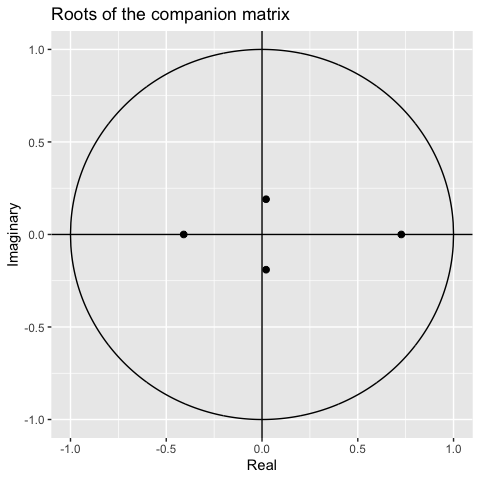
\includegraphics{12-exportedfigures/stability.plot-1} \end{center}
\vspace{-3mm}
\label{graf:stability}
\fonte{Desenvolvido a partir de dados coletados}
\vspace{-2mm}
\end{grafico}

Nos próximos parágrafos serão apresentados os resultados gerados pelo modelo PVAR-GMM, conforme a \autoref{tb:pvargmm}. O objetivo é primeiramente descrever os resultados, posteriormente comparar com as hipóteses geradas e por fim confrontar com outros estudos levantados.

\vspace{20pt}
\captionof{qdr}{Previsto e resultados}
\vspace{-2mm}
\linespread{2}

\begin{longtable}[]{@{}ccc@{}}
\toprule
& Previsto & Resultado \\
\midrule
\endhead
Hipótese & Variável & \(SprEp\) \\
:-----: & :---------: & :-------: \\
\(H_{1}\) & \(EPr_{it}\) & - \\
\(H_{2}\) & \(DepAv\) & - \\
\(H_{3}\) & \(DepAp\) & + \\
\(H_{4}\) & \(DepPop\) & + \\
\(H_{5}\) & \(DAdm\) & + \\
\(H_{6}\) & \(DesCap\) & + \\
\(H_{7}\) & \(OtDes\) & + \\
\(H_{8}\) & \(Inad\) & + \\
\(H_{9}\) & \(RcPd\) & + \\
\(H_{10}\) & \(ROpCr\) & - \\
\(H_{11}\) & \(RSrv\) & - \\
\(H_{12}\) & \(RPart\) & + \\
\(H_{13}\) & \(OtROp\) & + \\
\(H_{14}\) & \(OpEmp\) & - \\
\(H_{15}\) & \(OpFin\) & - \\
\(H_{16}\) & \(OtOp\)) & - \\
\(H_{17}\) & \(ImpRend\) & + \\
\(H_{18}\) & \(ImpInd\) & + \\
\(H_{19}\) & \(SelOvr\) & + \\
\(H_{20}\) & \(VelMo\) & - \\
\(H_{21}\) & \(Com\) & + \\
\(H_{22}\) & \(GrCon\) & + \\
\(H_{23}\) & \(IPCA\) & + \\
\(H_{24}\) & \(BMA\) & - \\
\(H_{25}\) & \(OpCrMkt\) & - \\
\bottomrule
\end{longtable}

\vspace{-7mm}

\label{qdr:previsto}
\fonte{Desenvolvido a partir do modelo}
\vspace{20pt}

\parindent 1.50cm

O \emph{spread ex-post} com 01 e 02 defasagem (\(lag1_SprEp\) e "\(lag2_SprEp\)) se demonstraram significativos somente com o próprio \emph{spread ex-post}. O resultado demonstra que o \emph{spread} de um período anterior atua de forma direta com \emph{spread} do período atual. Já o \emph{spread} de dois período anteriores atua de forma inversa com o \emph{spread} do período atual.

O resultado indica que, elevações no \emph{spread} em período anterior tendem provocar elevações no momento atual, porém em uma proporção menor do que ocorrido em período anterior, pois o \emph{spread} de dois períodos anteriores atua na redução do \emph{spread} no momento atual.

Em se tratando do spread defasado em um período (\(lag1_SprEp\)), este estudo chegou a resultado similar ao de \textcite{dantas:2012}, que encontrou significância estatística para o spread em período anterior com o spread de momento atual.

A rentabilidade defasada em um período (\(lag1_Rent\)) se demonstrou significativa para o \emph{spread ex-post}, atuando de forma indireta, e significativa para a rentabilidade, com relação direta. A rentabilidade defasada em dois períodos (\(lag2_Rent\)) se demonstrou significativa para o \emph{spread ex-post}, atuando de forma direta, e significativa para a rentabilidade, com relação direta.

De acordo com os resultados, elevações da rentabilidade de até dois períodos anteriores guardariam relação com elevações da rentabilidade para o período atual em proporções equivalentes. Elevações da rentabilidade em dois períodos exercem influência na elevação do \emph{spread}, mas em proporção menor que o efeito de redução exercido pela elevação da rentabilidade de período anterior.
Em nenhum dos estudos anteriores verificados foi identificada a utilização da rentabilidade como variável preditora para o \emph{spread} bancário \emph{ex-ante} ou \emph{ex-post}.

Para a participação das despesas administrativas nas operações de crédito (\(DAdm\)) foi remontada significância tanto para \emph{spread} bancário, atuando de forma direta, como para a rentabilidade com uma relação direta. O resultado no \emph{spread} para a variável está dentro o esperado, uma vez elevações nos custos evidentemente são repassados para os tomadores.

Os resultados do modelo para as despesas de captação se demonstraram relevantes tanto no \emph{spread}, quanto para a rentabilidade, ambos com uma relação direta. A relação sobre o \emph{spread} está dentro do esperado, porém a relação com a rentabilidade deve estar relacionada característica de gerar receita por nível despesa administrativa.

Os estudos de Koyama e Nakane (2001), Alfanasieff \emph{et. al.} (2001 e 2002) e Bignotto e Rodrigues (2006) encontraram significância estatística para os custos administrativos como determinante do \emph{spread ex-ante}. Já ao que remete o \emph{spread ex-post}, somente o estudo de \textcite{almeida:2013} foi encontrada significância para os custos administrativos.

Mesmo que, em comparação ao demais estudos, que utilizaram o volume dos custos administrativos, enquanto este estudo tenha utilizado o percentual destes custos em relação as operações de crédito, é possível afirmar que existem congruência lógica entre os resultados, validando assim o perfil de custos administrativos das instituições como um componente relevante do \emph{spread} bancário.

Para a proporção das despesas de captação em relação aos depósitos totais \(DesCap\) o modelo revelou elevada significância somente para o \emph{spread} bancário com uma relação direta. Esse resultado está dentro do esperado de acordo com as hipóteses teóricas. Não identificado, para fins de comparação, outro estudo que tenha utilizado esta variável ou outra análoga como preditora para o \emph{spread}

Os resultados para as despesas de captação \(DesCap\) implicam que em média, sempre que ocorre uma elevação ou redução nos custos de captação em relação aos depósitos totais, esse custo é repassado para a taxa de aplicação, fazendo com que o \emph{spread} bancário seja modificado em uma relação direta.

Para a participação de outras despesas em relação as operações totais (\(OtDes\)) o modelo remontou significância somente para o \emph{spread},com uma relação direta e expressiva, o que estava dentro do esperado, uma vez que esta variável comporta grandes montantes não segmentados e classificados. Não foram identificados outros estudos que tenham utilizado outras despesas como variável preditora para o spread.

O resultado para outras despesas (\(OtDes\)) implica que, em média, sempre que quando ocorre uma elevação ou redução desta participação em relação ao montante das operações totais, a oneração ou desoneração é repassada para a taxa de aplicação, desta forma modificando o \emph{spread} bancário em uma relação direta.

O resultado para participação da provisão de inadimplência sobre as operações totais (\(Inad\)) e risco ponderado de crédito (\(RcPd\)) foi de significância somente na rentabilidade com uma relação inversa. Mesmo sem significância, estas variáveis apresentaram relação direta com \emph{spread}.

O resultado implica que quando ocorrem elevações ou reduções na inadimplência e nível de risco de crédito, há um reflexo afetando na mesma direção a rentabilidade bancária, e de forma muito significativa.

A não significância estatística com o \emph{spread} pode estar associado com o fato de serem instrumentos de provisão. Outro possível resultado para a não significância pode se relacionar com composição do modelo e efeitos simultâneos, onde outras variáveis acabam por anularem a significância destas em ambas as variáveis.

Outras possível razão para a não significância da inadimplência e do risco de crédito está no fato de terem sido utilizas as variáveis no mesmo período que o \emph{spread}, desta forma alterações nas variáveis preditoras não causariam efeito sobre o \emph{spread} no mesmo período, mas sim um reflexo em períodos posteriores.

Para o risco de crédito, este estudo diverge do resultado apresentado por Bignotto e Rodrigues (2006), que encontraram significância, com esta variável e o \emph{spread ex-ante}, porém a mesma relação em termos de ajuste. Esta divergência também pode estar associada ao tipo a categoria de \emph{spread}, e mesmo as diferenças para obtenção desta variável, que neste estudo se utilizou uma média ponderada de risco.

Ainda para o risco de crédito, este resultado vem convergir com o de \textcite{almeida:2013}, que não encontrou significância em seu modelo que testou variável como preditora para o \emph{spread ex-post}. Em termos da relação o trabalho vem convergir com o resultado de \textcite{dantas:2012} que encontrou relação direta entre o risco de crédito e o \emph{spread ex-post}.

Para a significância da inadimplência este estudo diverge do resultado de \textcite{durigan:2018} para o \emph{spread ex-ante}, porém remontando a mesma relação em termos de ajuste. Tal divergência também pode estar associada a categoria de \emph{spread} utilizado e mesmo a diferença da forma de obtenção das variáveis entre os estudos.

Para a variável \emph{proxy} de participação do capital próprio em relação a operações totais (\(EPr\)) foi remontada significância para ambas as variáveis dependentes, com uma relação inversa com o \emph{spread ex-post} e inversa com a rentabilidade. Não foram identificados outros estudos que utilizaram alguma variável similar como preditora o para o \emph{spread}.

O resultado implica que, a medida que é elevada a participação do capital próprio para as operações de crédito totais, ocorre simultaneamente redução no \emph{spread} e na rentabilidade bancária. Os resultados remontados estão de acordo com a hipotese formulada.

A atuação do capital próprio sobre o \emph{spread} pode estar relacionado a ausência do pagamento de custos de captação, e mesmo com um elevado custo de oportunidade, atuaria reduzindo o \emph{spread}. Em relação a redução da rentabilidade pode estar associado ao custo de oportunidade e ao risco de se utilizar o capital próprio nas operações de crédito.

Para a variável de participação dos depósitos a vista sobre as operações totais (\(DepAv\)) foi remontada significância somente com a rentabilidade, em uma relação inversa. Mesmo sem significância, foi remontado uma relação inversa com o spread. Tais relações estariam dentro do esperado de acordo com as hipóteses formuladas, exceto a não significância com o spread.

Esse resultado implicaria que, no modelo, quanto maior a participação dos depósitos a vista, menor seria a rentabilidade bancária para o período. Tal resultado pode estar associado ao custo de oportunidade e risco de se utilizar depósitos a vista.

Mesmo sem significância com o \emph{spread}, a relação indicaria que quanto maior a participação de recursos captados via depósito a vista nas operações totais, menor seria o spread bancário. Tal relação pode estar associada a ausência de pagamento de juros de captação.

Este resultado vem divergir dos estudos de Afasieff \emph{el. al.} (2001) e Afasieff \emph{el. al.} (2002), que encontraram uma relação direta entre captações sem juros e o \emph{spread} bancário \emph{ex-ante}. Tal divergência poderia estar associada a diferença entre a forma do spread, bem como a forma da variável de captação utilizadas nos estudos.

Para a variável de participação dos depósitos a prazo em relação as operações totais (\(DepAp\))\footnote{Não foram identificados — para efeitos de comparação — outros estudos acerca do *spread* que se utilizaram de alguma variável similar a de depósitos a prazo.} O modelo não remontou significância, tanto para o spread como para a rentabilidade. Mesmo sem a significância o ajuste indicaria que esta variável, no ajuste do modelo, guardaria relação inversa com o \emph{spread} bancário e inversa com a rentabilidade.

O resultados do ajuste indicariam que quanto maior a participação dos depósitos a prazo, menores seriam o \emph{spread} e a rentabilidade bancária. A relação com o \emph{spread} estaria dentro do esperado na formulação das hipóteses, indicando que nem todos os custos de captação a prazo são repassados para a taxa de aplicação, reduzindo assim o \emph{spread}.

Para a participação dos depósitos de poupança em relação as operações totais (\(DepPop\))\footnote{Não foram identificados — para fins de comparação — outros estudos que utilizaram variável similar a esta como determinante do spread bancário.} foi remontadas significância somente para o \emph{spread}, com uma relação direta. O resultado para o spread está dentro do esperado, porém divergente para rentabilidade de acordo com as hipóteses formuladas.

Os resultados do ajuste indicam que quanto maior a participação dos depósitos de poupança, maior seria o \emph{spread} bancário e menor seria a rentabilidade. Tais relações podem ser explicadas pelas características quem envolvem as operações crédito que se encaixam esses recursos, bem como a modalidade, tipo de operação e nível de recolhimento compulsório cabíveis.

Para a variável de participação das receitas de operações de crédito em relação as receitas operacionais (\(ROpCr\))\footnote{Não foram encontrados — para fins de comparação — outros estudos que utilizaram variável similar como determinante do spread bancário} foi remontada significância para ambas as variáveis dependentes, sendo relação direta com o \emph{spread} e indireta com rentabilidade. O resultado para o spread está dentro do esperado de acordo com as hipóteses, não ocorrendo o mesmo para a rentabilidade.

O resultado do ajuste do modelo indica que quanto maior a participação das receitas de operação de crédito maior é o nível de \emph{spread} e menor é a rentabilidade das instituições. Tal resultado vem ressaltar que o nível de spread e rentabilidade guarda relação com o tipo de operação e capacidade de gerar receita de cada instituição.

Para a participação das receitas de serviços em relação a receitas operacionais (\(RSrv\)) o modelo remontou significância somente para o \emph{spread} bancário com uma relação direta, onde aumentos nas receitas de serviços estariam associadas a aumentos do \emph{spread}. Mesmo sem significância a variável apresentou relação direta com rentabilidade.

O resultado de ajuste do modelo indica que quando se eleva a participação da receita de serviços ocorrem aumento do \emph{spread} bancário e da rentabilidade bancária. Este resultado vem ressaltar a determinação do \emph{spread} e da rentabilidade diante as características operacionais de cada instituição e sua capacidade de gerar receita.

Este resultado para o \emph{spread} bancário vem convergir com os estudos de Afanasieff \emph{et. al.} (2002) e (2003), Bignotto e Rodrigues (2006) que encontram significância e uma relação direta das receitas de serviços com o \emph{spread} \emph{ex-ante} e divergir do estudo de \textcite{almeida:2013} que encontrou uma relação indireta com o \emph{spread ex-post}.

Para a relação entre as receitas de participação e as receitas operacionais (\(RPart\))\footnote{Não foram identificados — para fim de comparação  — outros estudo que utilizaram variável similar a esta como determinante do \emph{spread}} o modelo retorno significância com ambas as variáveis dependentes, sendo uma relação direta com o \emph{spread} e inversa com a rentabilidade. Diante a formulação das hipóteses, o resultado para o spread está dentro do esperado, mas diverge para a rentabilidade, onde se esperava o contrário.

Este resultado implica que quanto maior a parcela das receitas de participação das instituições maior é o \emph{spread} aplicado em suas operações, mas por outra via essa característica atuaria reduzindo a rentabilidade, talvez associado a prejuízos operacionais, denotando novamente os aspectos operacionais na determinação destas duas variáveis.

Para a participação de outras receitas operacionais diante as receitas operacionais (\(OtROp\))\footnote{Não foram identificados — para fim de comparação — outros estudos que tenham utilizado alguma variável similar como determinante do \emph{spread bancário}} o modelo retornou significância para somente com o \emph{spread}, com uma relação direta. Mesmo sem significância, retornou uma relação direta com a rentabilidade. O resultado, diante as hipóteses formuladas, está dentro do esperado.

O resultado implica que quanto maior a receita proveniente de outras operações, maior seria o nível de \emph{spread} praticado, e mesmo sem significância o resultado do ajuste indica que maior seria o nível de rentabilidade. Um maior nível de spread associado a um maior nível de rentabilidade pode estar associado a um poder de mercado das instituições, cobrando elevados juros com reduzidos custos operacionais.

O resultado do modelo de outras operações em relação ao \emph{spread} apresentou um dos maiores níveis de significância e de impacto no ajuste da relação entre as variáveis.

Para as participações de operações\footnote{Não foram identificados — para fim de comparação — outros estudos que utilizaram variáveis similares a esta como determinantes do \emph{spread}} de empréstimo (\(OpEmp\)) e operações de Financiamento (\(OpFin\)) diante as operações totais o modelo retorno significância somente para a rentabilidade, com uma relação inversa, e direta com o spread. Já a participação de outras operações (\(OtOp\)) diante as operações de crédito retornou significância somente com o spread com uma relação direta, e inversa com a rentabilidade.

O resultados implicam que, diante as significâncias remontadas, quanto maior a participação operações de empréstimos (\(OpEmp\)) e financiamentos (\(OpFin\)) menor seria o nível de rentabilidade e quando maior o nível de outras operações (\(OtOp\)), maior seria o nível de \emph{spread}, o que poderia estar associado as características destas operações e ao poder de mercado das instituições que a realizam.

No ajuste as participações operações de empréstimos (\(OpEmp\)) e financiamentos (\(OpFin\)) atuariam reduzindo a rentabilidade em uma proporção superior a redução causada por outras operações (\(OtOp\)), em relação a spread, o ajuste indica esta última exerce influência em proporção maior que as outras duas operações.

Para os impostos indiretos (\(ImpInd\)) e impostos sobre a renda (\(ImpRend\))\footnote{Não foram identificados — para fim de comparação — outros estudos que utilizaram variável similar a esta como determinante do spread bancário} o modelo retornou significância somente para a rentabilidade. Os impostos indiretos apresentaram relação direta. Já os impostos sobre a renda apresentaram uma relação inversa com a rentabilidade.

Esse resultado implicaria que quanto maior o nível de impostos indiretos, maior seria a rentabilidade das instituições. Esse resultado pode estar relacionado capacidade de gerar receita por operação tributada. A não significância com o \emph{spread} pode estar ligada com o fato destes estarem embutidos na taxa de juros e ainda serem instrumento de provisão e passíveis de recuperação, onde o ônus seria repassado para o tomador.

O resultado para os impostos indiretos vem convergir com o resultado encontrado por \textcite{almeida:2013}, que não encontrou significância deste variável com o \emph{spread ex-post}. Porém diverge dos resultados encontrados por Koyama e Nakane (2001a e 2001b) e Afanasieff \emph{et. al.} (2001 e 2002), que encontraram significância e uma relação direta entre os impostos indiretos e o \emph{spread ex-ante}.

O resultado para os impostos sobre a renda implicariam que quanto maior nível destes, menor seria o nível rentabilidade das instituições. O que ocorre por serem impostos que são cobrados diante os resultados das instituições, de forma direta.

A não apresentação significância estatística e a relação inversa dos impostos indiretos e impostos sobre a renda com o spread na modelagem não as desqualificam como componente implícito consolidados e determinantes do spread bancário, como identificado em \textcite{BACEN} e cardoso:1999. O resultado implica em uma influência simultânea na rentabilidade e ação de outras variáveis na modelagem.

Para a variável Selic Over (\(SelOvr\)) o modelo remontou significância para ambas as variáveis dependentes, com relação inversa com o \emph{spread} e também inversa com a rentabilidade. O resultado para a rentabilidade está dentro do esperado, porém divergente para o \emph{spread}, diante do que foi definido nas hipóteses prévias.

Os resultados implicam que elevações na Selic over de três períodos anteriores levariam a reduções no nível de spread no momento atual. Esse resultado pode estar associado ao não repasse de custos de captação à taxa de aplicação no curto prazo. Os resultados implicariam que elevações na Selic over defasada atuariam reduzindo a rentabilidade bancária do período atual.

Esse resultado vem divergir dos estudos de Koyama e Nakane (2001a e 2001b), Afanasieff \emph{et. al.} (2001 e 2002), \textcite{oreiro-2006} e \textcite{durigan:2018} que encontram relação direta e significativa da Selic com o spread bancário. Tal divergência pode estar associada as diferenças metodológicas e função da variável nas modelagens.

O resultado vem a convergir com os resultados do estudo de \textcite{BCB:1999}, que menciona que após mudanças de políticas cambiais. fiscais e monetárias após 1999, os juros e spread não ficaram mais sensíveis a volatilidade da taxa de juros básica.

Para a variável de velocidade da moeda (\(VelMo\))\footnote{Não foram identificados — para fim de comparação — outros estudos que utilizaram variável similar a esta como determinante do spread bancário}, o modelo remontou significância para ambas as variáveis dependentes, com relação direta com \emph{spread} a também direta para rentabilidade. O resultado está dentro do esperado pela definição das hipóteses prévias.

O resultado implica que elevações da velocidade da moeda --- crescimento do PIB maior que crescimento da base monetária --- elevaria tanto o spread bancário como a rentabilidade bancária. Isso ocorreria, pois em momentos de aquecimento da economia a sensibilidade ao repasse de juros e custos e lucro se reduziriam.

Para o nível de compulsório das operações (\(Comp\)), o modelo remontou apresentou significância estatística apenas com o spread, com uma relação direta e uma relação inversa com a rentabilidade bancária. O resultado para o spread está dentro do esperado na definição das hipóteses, porém se esperava significância para a rentabilidade, em uma relação inversa.

O resultado implica que elevações na taxa de compulsório --- que elevam a necessidade de captação para uma operação de crédito --- atuariam elevando o nível de spread bancário.

Este resultado vem convergir com o estudo de Afanasieff \emph{et. al.} (2002) que encontrou relação direta entre o compulsório e spread, e divergir de Afanasieff \emph{et. al.} (2001) que encontrou uma relação inversa. Tais diferenças entre os estudos podem estar associadas as diferenças metodológicas e a função da variável nos diferentes modelos utilizados.

O modelo não remontou significância para o grau de concentração do mercado (\(GrCon\)), porém o resultado demonstra uma relação inversa com o \emph{spread} e direta com a rentabilidade. Este resultado vem divergir dos estudos de \textcite{dantas:2012} e \textcite{almeida:2013}, que encontraram significância e uma relação direta com o grau de concentração e o \emph{spread ex-post}.

Diante a composição do modelo, para a IPCA foi remontada significância somente para o spread, com relação inversa e relação inversa com a rentabilidade. Os resultados estão dentro do esperado na formulação da hipóteses, porém se esperava significância para ambas as variáveis.

O resultado implica que elevações na inflação atuariam na redução do nível de spread bancário. A inflação pode atuar corroendo a taxa de aplicação e elevando a taxa de captação, reduzindo assim o spread e consequentemente a rentabilidade.

Este resultado vem convergir com os estudos de Bignotto e Rodrigues (2006) e \textcite{durigan:2018} que encontram relação significativa e direta entre IPCA e o \emph{spread ex-ante} e divergir do estudo de \textcite{aronovich:1994} que encontrou relação direta entre estas variáveis.

Para os meios de pagamentos ampliados 4 (\(lnMPA4\))\footnote{Não foram identificados — para fim de comparação — outros estudos que utilizaram variável similar a esta como determinante do spread bancário} o modelo remontou significância somente sobre o \emph{spread} com uma relação direta. E mesmo sem significância a relação com a rentabilidade foi direta. O resultado diverge do esperado na formulação das hipóteses.

O resultado implicaria que elevações no volume do agregado monetário M4 de três períodos anteriores, refletiriam em elevações no spread bancário no momento atual.

Para o volume de operações de crédito do mercado (\(lnOpCrMkt\))\footnote{Não foram identificados — para fim de comparação — outros estudos que utilizaram variável similar a esta como determinante do spread bancário} o modelo remontou significância somente para o \emph{spread}, com uma relação inversa, e mesmo sem significância retornou uma relação direta com rentabilidade. As relações estão dentro do esperado durante a formulação da hipoteses.

O resultado implica que elevações no volume de operações totais do mercado bancário atua exercendo redução no nível de spread, ao mesmo tempo que elevaria a rentabilidade. Tal resultado pode estar relacionado com a capacidade de instituições que possuam maior fatia de mercado em operar com um nível de juros menor, visando ganhar no volume de operações.

\section{Função Impulso resposta}

No \autoref{graf:impulseorto} está demonstrada a função impulso-resposta ortogonal com os intervalos de confiança gerados por bootstrapping. Indicando que um choque estrutural na rentabilidade tem efeito significativo e inverso sobre o spread e que um choque estrutural no spread tem um efeito quase nulo sobre a rentabilidade.

\vspace{20pt}

\begin{grafico}[!htbp]
\caption{Função de impulso resposta ortogonal}
\vspace{-4mm}

\begin{center}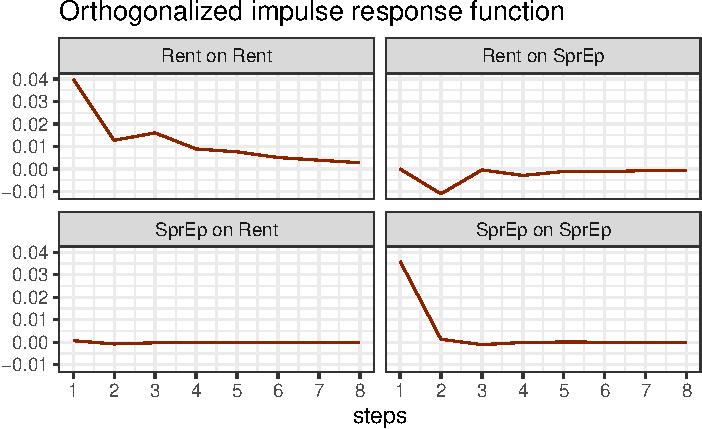
\includegraphics{12-exportedfigures/impulse.plot.orto-1} \end{center}
\vspace{-3mm}
\label{graf:impulseorto}
\vspace{-2mm}
\fonte{Desenvolvido a partir dos resultados do modelo }
\end{grafico}

\textual
\pagestyle{simple}
\parindent 1.50cm

\chapter{CONSIDERAÇÕES FINAIS}

Este estudo teve como objetivo verificar os principais conceitos e aspectos técnicos sobre o \emph{spread} bancário e como os seus principais determinantes atuam de forma simultânea influenciando a rentabilidade bancária, alinhado com as perspectiva de importância do \emph{spread} na atividade econômica e na estabilidade do setor financeiro.

O ponto de partida foi a investigação sobre os principais aspectos do setor bancário brasileiro, verificando a tendência para concentração bancária, domínio de instituições estrangeiras, baixa oferta de crédito, baixa relação crédito PIB, baixo grau de alavancagem financeira diante elevados níveis de inadimplência e risco de crédito.

Também foram verificadas as principais características da estrutura bancária no Brasil, estando esta inserida no Sistema Financeiro Nacional, organizado em modalidades por tipo de carteira de operação com uma tendência a partir da década de 1980 de concentração de instituições atuando com operações de múltiplas carteiras.

Foi identificado que o \emph{spread} bancário tem ganhando notoriedade a nível mundial por se tratar de um indicador que de elevada importância com o desenvolvimento e crescimento econômico bem como na manutenção de um sistema financeiro sólido, competitivo e com liquidez.

Durante o estudo verificou-se que o conceito consolidado do \emph{spread} se dá pela diferença entre as taxas de aplicação --- cobrada dos tomadores de crédito --- e a taxa de captação --- que remunera as captações ---. Por outra perspectiva implica na diferença entre o juros cobrado dos clientes e a juros pagados aos depositantes.

Verificou-se que não há uma teoria formalizada acerca do spread bancário, mas seus estudos vem sendo sistematizados em torno da evolução, estrutura e componentes, de acordo com abrangência da amostra, conteúdo e origem da informação, onde esta última concerne nos conceitos de \emph{spread ex-ante} --- medida de planejamento --- e o spread \emph{ex-post} --- medida de resultado ---.

Em relação as diferenças conceituais entre \emph{spread} ex-ante e ex-post, o primeiro por ser uma medida de planejamento se torna mais instável, volátil e sensível a indicadores de conjuntura econômica e o seguindo por ser medida de resultado se demonstra mais estável e menos sensível a indicadores macroeconômicos.

O método consolidado de apuração do \emph{spread} leva e consideração a participação das receitas das operações de crédito sobre o total de capital emprestado menos a relação entre os custos de captação em relação aos depósitos totais. E que entre os principais componentes endógenos estão as despesas administrativas, impostos indiretos, impostos diretos, despesas de captação, inadimplência e a margem de lucro.

Foi identificado que entre os principais determinantes exógenos utilizados para o \emph{spread} estão a atividade econômica, PIB, atividade industrial, PIB Industrial, IPI, desemprego, Selic, IPCA, compulsório e saldo da carteira de crédito.

Durante o período investigado foi levantando que o \emph{spread} bancário no Brasil figura entre um dos maiores a nível mundial e mesmo com considerável redução --- de um nível que chegou a representar 150\% --- ainda é considerado elevado principalmente se comparando com países com mesmo grau de desenvolvimento.

Ao longo do estudo foi identificado que o \emph{spread} pode ser visualizado em diferentes perspectivas no que tange a dimensão por tipo de tomador ou tipo de recurso e operação ou na perspectiva volume-prazo-risco que abrange os níveis de spread por volume de recurso, tempo de tomada, riscos e a existência ou não de garantias.

Diante os conceitos, detalhes técnicos e óticas do \emph{spread}, foi realizado um ensaio de decomposição, partindo da forma tautológica do \emph{spread}, incluindo as variáveis endógenas componentes para fins de identificação destas, chegando a formulação de um multiplicador de aplicação na ótica do dispêndio e multiplicador de capital emprestado na ótica do juros.

Uma modelagem baseada na decomposição do \emph{spread} e diante as óticas de estudo, ótica de dimensão, ótica de volume-tempo-risco se apresentaria com a ideal para uma estudo com maior acurácia. Porém diante do nível de informações disponível não é possível atingir este nível de estudo, cabendo assim a modelagem a apartir dos dados disponíveis, em nível de agregação elevados.

A primeira rodada de teste realizou modelagem nos métodos \emph{pooling}, efeitos fixos e efeitos aleatórios, remontando coeficientes de determinação acima de 90\% para ambos, porém os modelos não passaram no teste de heterocedasticidade e correlação serial, prejudicando assim a confiabilidade dos mesmos.

Seguindo a complexidade da modelagem partiu-se o método de painel dinâmico com vetores autorregressivos com estimação por método dos momentos generalizados em duas etapas, com transformação ortogonal para frente e utilização de instrumentos PCA com 18 variáveis endógenas e 7 variáveis exógenas.

O modelo com duas defasagens da variáveis dependentes foi selecionado pelo teste de seleção por critérios de momentos (MMSC). O modelo passou pelo teste J-Hansen de superidentificação de restrições, aceitando-se a hipótese nula de validade de todas as variáveis no modelo.

As variáveis que apresentaram significância simultaneamente no \emph{spread} e na rentabilidade foram a rentabilidade com uma e duas defasagens, as despesas administrativas, receitas de operação de crédito, receitas de participação Selic over, e velocidade da moeda.

Entre as principais variáveis determinantes que exercem influência direta no \emph{spread} estão, em ordem de peso: outras despesas operacionais, as receitas de operação de crédito, outras receitas operacionais, despesas administrativas, velocidade da moeda e receita de serviços.

O segundo bloco de variáveis determinantes que exercem influência direta no \emph{spread} estão: a rentabilidade de dois períodos anteriores, outras operações, depósitos de poupança, meios de pagamento M4, receita de participação, spread de um período anterior e o compulsório.

Entre as variáveis que apresentaram influência inversa no \emph{spread},em ordem de peso estão: Selic Over, IPCA, \emph{spread} de dois períodos anteriores, capital próprio, operação total do mercado e rentabilidade de um período anterior.

Já na rentabilidade entre as variáveis que exercem influência direta, em ordem de peso, estão: Rentabilidade de um e dois períodos anteriores, velocidade da moeda, impostos indiretos e despesas administrativas.

Entre as variáveis que apresentaram influência inversa com a rentabilidade, em ordem de peso estão: imposto de renda, receita de operações de crédito, Risco ponderado de crédito, operações de crédito, operações de financiamento, inadimplência, depósitos a vista, receitas de participações e Selic over.

Os resultados do modelo remetem que o \emph{spread} e a rentabilidade são determinados uma parte diante um conjunto de características e do perfil operacional das instituições bancárias em torno de seus elementos endógenos e por outra parte determinado por fatores exógenos de mercado e de conjuntura econômica.

Como principal determinante direto do \emph{spread}, o modelo retornou a variável de participação de outras despesas em relação as operações de crédito (1,2571), em um nível muito significativo. Quanto maior o nível desta variável, maior seria o nível de \emph{spread} bancário.

Como segunda e terceira variável com influência direta no \emph{spread} aparecem a receita de operações de crédito e outras receitas operacionais. Dessa forma, instituições tem possuem maior capacidade e suas receitas baseada nestas operações apresentam maior nível de \emph{spread} bancário.

Por outra via o modelo retornou que as receitas com operações de crédito está entre os principais determinantes indiretos da rentabilidade. Ou seja, quando maior o nível desta variável, maior o \emph{spread}, porém menor seria a rentabilidade das instituições.

Como quarto e quinto principais determinantes diretos do \emph{spread} o modelo remontou as despesa de captação e as despesas administrativas. O que leva a conclusão que as instituições que possuem maior nível destas despesas, acabam por apresentar os maiores níveis de \emph{spread}, levando ainda a característica que esses custos são em grande parcela repassados para a taxa de juros.

Na perspectiva de atuação simultânea, o modelo retornou que as despesas administrativas atuam como principal principal determinante direto da rentabilidade, ou sejam quando maior o gasto com despesas administrativas, maior a capacidade das instituições e aumentar a rentabilidade, reforçando a característica desse custos ser quase que totalmente repassado sem afetar a margem de lucro.

Como sexto principal determinante direto do \emph{spread} o modelo retornou a velocidade da moeda. Por outra via a velocidade da moeda se apresenta também como o principal\footnote{Sem considerar as variáveis defasadas da própria rentabilidade} determinante direto da rentabilidade. Quanto mais rápido uma unidade monetária circula na economia, maior será o nível de \emph{spread} e rentabilidade das instituições bancárias.

Como sétimo principal determinante direto do \emph{spread} aparece as receitas de serviços. Esse resultado implica que quando maior a concentração de receitas de serviços a instituição possuir, maior será o nível de \emph{spread} bancário cobrado por estas.

Mesmo sem significância, a inadimplência e o risco ponderado de crédito aparecem no ajuste do modelo como determinantes em nível direto do \emph{spread} bancário. Por outras via estas variáveis apresentaram significância como determinantes indiretas da rentabilidade. Isso remete que elevações do nível de inadimplência e careteiras com maior risco ponderado atuam elevando o \emph{spread} e reduzindo a rentabilidade.

Entre outras variáveis ligadas as características operacionais, que atuam determinantes diretas do \emph{spread}, em menor nível estão outras operações\footnote{Significância somente para o spread}, depósitos de poupança\footnote{Significância somente para o spread}, operações de empréstimo\footnote{Significância somente para a rentabilidade}, receita de participação e operação de financiamento\footnote{Significância somente para a rentabilidade}. Elevações destas variáveis atuariam elevando o nível de spread bancário.

Das variáveis do parágrafo anterior, mesmo que nem todas apresentassem significância, o efeito sobre a rentabilidade seria inverso. Ou seja, quanto maior o nível destas variáveis menor seria o nível de rentabilidade.

Entre as variáveis exógenas que exercem influência direta sobre o \emph{spread} estão o agregado monetário M4 e o compulsório. Mesmo sem significância estas variáveis também apresentaram relação direta com a rentabilidade. Elevações no M4 e no compulsório levariam e aumento do \emph{spread} e da rentabilidade bancária.

No modelo, o principal determinante indireto do \emph{spread}, seria a rentabilidade auferida em período anterior. Esta variável também atuaria como determinante direto da rentabilidade. Dessa forma quando ocorrem elevações de rentabilidade no período atual o reflexo seria de redução do \emph{spread} atual, porém com manutenção de certo nível de rentabilidade, podendo estar associado a diluição de custos operacionais ao longo do prazo.

Entre as variáveis exógenas que, no modelo, exercem influência indireta no \emph{spread} estão o grau de concentração\footnote{Sem significância para o spread e rentabilidade}, operação total do mercado\footnote{Significância para o spread}, IPCA\footnote{Significância para o spread}, impostos indiretos\footnote{Significância para a rentabilidade}, Selic over e imposto de renda\footnote{Significância para a rentabilidade}. Elevações destas variáveis atuariam reduzindo o \emph{spread} bancário.

Para o IPCA, impostos indiretos e imposto de renda a relação inversa com o \emph{spread} pode ser explicada pelo não repasse total de elevações destas para a taxa de juros. Dessa forma mantida a estrutura de custos e não repasse destes, o resultado observado seria uma redução de \emph{spread}.

No grupo de variáveis endógenas o capital próprio\footnote{Significância para o spread}, \emph{spread} de dois períodos anteriores\footnote{Significância para o spread}, depósito a prazo\footnote{Sem significância para o spread e rentabilidade} e deposito a vista\footnote{Significância para a rentabilidade} exercem, no modelo, uma influência inversa com o \emph{spread} e com a rentabilidade. Elevações destas variáveis atuariam reduzindo o \emph{spread} --- via taxa de aplicação --- e reduzindo também a rentabilidade --- devido a redução na taxa de aplicação ---.

Entre as variáveis exógenas com efeito inverso sobre o \emph{spread} bancário, o IPCA, Selic over e imposto de renda também manteriam relação inversa com a rentabilidade, já o grau de concentração, operação total de mercado e impostos indiretos\footnote{Esta relação poderia estar associada ao fato de ser um imposto sobre a venda com baixa sensibilidade do consumidor} manteriam relação direta com a rentabilidade.

Diante o resultado da pesquisa e da modelagem econométrica este estudo chega ao conceito que o \emph{spread} e a rentabilidade bancária são definidos diante um conjunto de fatores endógenos remetendo as características operacionais de cada grupo e ou instituições e diante um conjunto de fatores exógenos relacionados com a conjuntura social e econômica e de regulação.

A contribuição desta pesquisa está na utilização de variáveis endógenas determinantes do \emph{spread}, que representam as características operacionais da empresas diante um conjunto de fatores que implicam no tipo de operação, capacidade de gerar receita, origem do capital e eficiência operacional.

Para estudos posteriores fica a indicação para avaliação dos efeitos dos determinantes do \emph{spread} atuando simultaneamente sobre a taxa de aplicação, taxa de captação e rentabilidade bancária. Ainda a orientação de trabalhar os dados no maior nível de desagregação possível para visualização do nível por tipo de tomador, tipo de operação, tipo de recurso, volume, prazo e nível de risco, levando consideração que no momento da pesquisa este nível não está disponível.

\postextual

\addcontentsline{toc}{chapter}{REFERÊNCIAS}
\printbibliography[title={REFERÊNCIAS}]

\postextual

\addtocontents{toc}{\vspace{-2pt}}

\ifthenelse{\equal{\terApendice}{Sim}}

\{

\begin{apendicesenv}

\vspace{-10mm}

\renewcommand{\thechapter}{\arabic{chapter}}

\chapter{Decomposição do Spread}\label{apendicea}

Este apêndice tem como propósito realizar a decomposição algébrica do *spread* com objetivo de inserir e identificar variáveis componentes à partir de definições teóricas e técnicas, dentro das perspectivas de ótica, características, dimensão e volume-prazo-risco abordadas na \autoref{sec:spread}.

A decomposição parte da definição geral tautológica de *spread* ($Spr$), como resultado da diferença entre a taxa de aplicação ($I_{apl}$) e a taxa de captação ($i_{cap}$), representada na \autoref{spr:taut}.



\begin{equation}\label{spr:taut}
Spr = i_{apl} - i_{cap}
\end{equation}



Em termos de resultado a taxa de aplicação ($i_{apl}$) é obtida da relação entre a receita operacionais ($R$) e das operações de crédito ($E$). Já a taxa de captação é extraída da relação entre as despesas de captação ($DC$) e o montante capitado ($C$), conforme representado na \autoref{eq:aplcap}


\begin{equation}\label{eq:aplcap}
i_{apl} = \frac{R}{E}  \hspace{10pt} |  \hspace{10pt} i_{cap} =  \frac{DC}{C}  \hspace{10pt} |  \hspace{10pt} Spr =  \frac{R_{}}{E} -  \frac{DC}{C}
\end{equation}


As receitas operacionais das instituições financeiras se dividem em: 1) Receitas de Operações de Crédito ($ROpCr_{}$); 2) Rendas De Cambio ($RCamb$) ; 3) Rendas De Aplicacoes Interfinanceiras De Liquidez($RApIf$); 4) Rendas Com Títulos E Valores Mobiliários E Instrumentos Financeiros Derivativos ($RMobDer$); 5) Rendas De Prestação De Serviços ($RSrv$); 6) Rendas De Participações ($RPart$) e 7) Outras Receitas Operacionais ($OtROp$) \autoref{eq:receitas}.


\begin{equation}\label{eq:receitas}
ROp_{} = R_{OpCr} + R_{Camb} + R_{ApIf} + R_{MobDer} + R_{Srv} + R_{Part} + R_{Ot}
\end{equation}


Para fins de estudo podemos separar as receitas das operações de crédito ($ROpCr_{}$) das outras receitras operacionais ($OtRop$) conforme demonstrado nas \autoref{eq:receitas2} e  \autoref{eq:receitas3} 


\begin{equation}\label{eq:receitas2}
OtROp = R_{Camb} + R_{ApIf} + R_{MobDer} + R_{Srv} + R_{Part} + R_{Ot} 
\end{equation}

\begin{equation}\label{eq:receitas3}
ROp = ROpCr_{} + OtRop
\end{equation}

A receita das operações de crédito ($ROpCr$) é obtida levando em  consideração as operações de crédito — capital emprestado — ($E$) e uma taxa de juros ($i_{jr}$), visualizada na \autoref{eq:recind}. A taxa de juros contempla os custos de captação, os custos operacionais, inadimplência, risco, impostos diretos e indiretos e margem líquida, conforme levantamento na \autoref{sec:spread}.



\begin{equation}\label{eq:recind}
ROpCr_{} = Ei_{jr}
\end{equation}



A receita de operações de crédito ($ROpCr_{}$) pode ser decomposta, diante os elementos que constituem a base da taxa de juros,  englobando as despesas operacionais e administrativas ($DAdm$), provisões de inadimplência ($Inad$) custos de captação ($DC$), impostos indiretos ($ImpInd$), impostos sobre a renda ($ImpDir$) e margem líquida ($MgLqd$), conforme identificado na \autoref{sec:spread}.



\begin{equation}
ROpCr_{} = DAdm + Inad + DC + ImpInd + ImpDir + MgLqd
\end{equation}


A decomposição da receita pode ser ampliada com a inserção das respectivas bases de incidências conforme a \autoref{eq:decrec}\footnote{Considerando que não são abatidos os custos operacionais da base de arrecadação do PIS e COFINS, conforme \textcite{cardoso:1999}}\footnote{São abatidos da base do IR e CSLL os custos com o FGC, conforme \textcite{cardoso:1999}}\footnote{Incluindo a compensação de 1/3do COFINS na CSLL, conforme \textcite{cardoso:1999}}, forma similar com que é apresentado em \textcite{cardoso:1999}, em estudo da cunha fiscal sobre o \emph{spread} bancário. 

O primeiro bloco da decomposição da receita na se refere às taxas e alíquotas aplicados sobre o capital emprestado ($E$) e captação ($C$), sendo elas as despesas administrativas ($i_{adm}$), inadimplência ($i_{ind}$), captação ($i_{cap}$), recolhimento compulsório ($i_{comp}$), aplicação de compulsório($i_{ac}$) e fundo garantidor de crédito ($i_{fgc}$).

O segundo bloco da decomposição da receita na \autoref{eq:decrec} consiste na inseção de variáveis referente as taxas e alíquotas aplicados sobre a própria receita da operação de crédito ($ROpCr_{}$), contemplando o PIS ($i_{pis}$), IOF ($i_{IOF}$), COFINS ($i_{cof}$), imposto de renda ($i_{ir}$), contribuição social ($i_{cs}$) e lucro líquido ($i_{ll}$), formando o \emph{markup} das instituições.



\begin{equation}\label{eq:decrec}
\begin{aligned}
ROp_{} \hspace{10pt} = \hspace{10pt} &  i_{adm}E + i_{ind}E + i_{iof}E + i_{cap}C + i_{comp}i_{ac}C + i_{fgc}C + \frac{i_{ll}}{1 - i_{r} - i_{cs}}ROpCr_{} + i_{pis}ROp_{} \\ 
& + i_{cof}ROp_{} +  i_{r} [ROp_{}(1-i_{pis} - i_{cof}) - 0,01] + i_{cs} [ROp_{}(1-i_{pis} - i_{cof}) - i_{fgc}]
\end{aligned}
\end{equation}

  
Levando em consideração que os depósitos são reduzidos diante a obrigação de recolhimentos compulsórios e contribuição para o fundo garantidor de crédito (FGC), um empréstimo ($E$) que dependa de captação ($C$), a necessidade de captação será maior para atender a operação de empréstimo no volume almejado, conforme demonstrado na \autoref{eq:nesscap} \cite{cardoso:1999}.



\begin{equation}\label{eq:nesscap}
C = \frac{E}{(1 - i_{comp} - i_{fgc})}
\end{equation}


Diante a inseção dos componentes explícitos da receita das operações de crédito ($ROpCr$), o passo seguinte consiste em isolar à esqueda os componentes incidentes sobre a receita e evidenciar variáveis em comum em ambos os lados da equação. Substituindo \autoref{eq:nesscap} em \autoref{eq:decrec}, obtemos as parciais em \autoref{eq:decrec2} e \autoref{eq:recpar02}. 


\begin{equation}\label{eq:decrec2}
\begin{aligned}
& ROp_{} \left[ 1 - \frac{i_{ll}}{1 - i_{r} - i_{cs}} - i_{pis} - i_{cof} - i_{r} (1-i_{pis} - i_{cof} - 0,01) - i_{cs} (1-i_{pis} - i_{cof}) \right] = \\
& i_{cap} \left[ \frac{E}{1 - i_{comp} - i_{fgc}} \right] + i_{adm}E + i_{Inad}E + (1 - i_{ir} - i_{cs})i_{IOF}E + i_{fgc} \left[ \frac{E}{1 - i_{comp} - i_{fgc}} \right] + \\ & i_{cs}i_{fgc}\left[\frac{E}{1 - i_{comp} - i_{fgc}}\right] - 
i_{r}i_{fgc}\left[\frac{E}{1 - i_{comp} - i_{fgc}}\right] + i_{ac}i_{comp}\left[\frac{E}{1 - i_{comp} - i_{fgc}}\right]
\end{aligned}
\end{equation}




\begin{equation}\label{eq:recpar02}
\begin{aligned}
& ROpCr_{}\left[ 1 - \frac{i_{ll}}{1 - i_{r} - i_{cs}} - i_{pis} - i_{r}i_{pis} - i_{pis}i_{cs} - i_{cof} - i_{r}i_{cof} - i_{cof}i_{cs} - i_{r} - 0,01i_{r} - i_{cs}\right] = \\
& E [ i_{adm} + i_{Inad} + i_{IOF} +  i_{cap}\frac{1}{1 - i_{comp} - i_{fgc}} + i_{fgc}\frac{1}{1 - i_{comp} - i_{fgc}} + i_{ac}i_{comp}\frac{1}{1 - i_{comp} - i_{fgc}} - \\
& i_{r}i{fgc}\frac{1}{1 - i_{comp} - i_{fgc}} + i_{cs}i_{fgc}\frac{1}{1 - i_{comp} - i_{fgc}} ]
\end{aligned}
\end{equation}


Ao evidenciar os termos em comum referentes aos impostos indiretos e operações de crédito obtemos a terceira parcial em \autoref{eq:recpar03}



\begin{equation}\label{eq:recpar03}
\begin{aligned}
& ROpCr_{}\left[1 - (\frac{i_{ll}}{1 - i_{r} - i_{cs}} + i_{pis}(1 - i_{r} - i_{cs}) + i_{cof}(1 - i_{r} - i_{cs}) + 0,99i_{r} + i_{cs})\right] = \\
& E\left[i_{adm} + i_{Inad} + i_{IOF} +  [\frac{1}{1 - i_{comp} - i_{fgc}}] (i_{cap} + i_{fgc} + i_{ac}i_{comp} - i_{r}i{fgc}+ i_{cs}i_{fgc})\right]
\end{aligned}
\end{equation}



Isolando a receita à esquerda e realizando as manipulações algébricas, introduzindo para cada período de tempo ($t$) a perspectiva de dimensão envolvendo tipo de tomador($a$), tipo de recurso ($b$) e modalidade da operação ($c$), tipo de operação ($d$), origem do capital ($e$) as taxas de sensibilidade às perspectivas de volume ($v$), prazo ($p$), risco ($r$) e garantia ($g$), obtemos a \autoref{eq:recend}.

O \emph{spread} ainda pode ser visualizado de acordo com as diferentes operações ($d$) , sendo elas: 1) Empréstimos e Direitos Creditórios Descontados; 2) Financiamentos; 3) Financiamentos Rurais) 4) Financiamentos Mobiliários; 5) Operações De Credito Vinculadas A Cessão 6) Avais E Fianças Honrados; 7) Carteira De Cambio; 8) Rendas A Receber; 9) Negociação E Intermediação De Valores; 10) Créditos Específicos e 11) Diversos.

A origem de capital ($e$) a ser emprestado ($E$), pode assumir a forma de capital próprio ($Pr$), depósito a vista ($Av$), depósito à prazo ($Ap$) depósito interfinanceiro ($If$), depósito de poupança ($Pop$) e outros depósitos ($OtD$)



\begin{equation}\label{eq:recend}
\begin{aligned}
R_{Op[t,a,b,c,d,e]} = & \frac{E_{} \left[ i_{adm} + i_{Inad} + i_{IOF} + r +  \frac{(i_{cap} + i_{fgc} + i_{ac}.i_{comp} - i_{r}.i_{fgc}+ i_{cs}.i_{fgc})}{1 - i_{comp} - i_{fgc}} \right]}
{\left[ 1 - (\frac{i_{ll}}{1 - i_{r} - i_{cs}} + i_{pis}(1 - i_{r} - i_{cs}) + i_{cof}(1 - i_{r} - i_{cs}) + 0,99i_{r} + i_{cs})\right]}vpg
\end{aligned}
\end{equation}



O numerador da \autoref{eq:recend} remete aos dispêndios das operações de crédito ($D$), visualizado de forma isolada em \autoref{eq:num}, para cada perspectiva operacional.


\begin{equation}\label{eq:num}
D_{t[a,b,c,d,e]} = E_{} \left[ i_{adm} + i_{Inad} + i_{IOF} + r +  \frac{(i_{cap} + i_{fgc} + i_{ac}i_{comp} - i_{r}i_{fgc}+ i_{cs}i_{fgc})}{1 - i_{comp} - i_{fgc}} \right]
\end{equation}



Na ótica dos dispêndios, o denominador da \autoref{eq:recend}, ao ser manipulado algebricamente, assume a função de multiplicador das despesas e custo de captação ou *markup* ($i_{mkp}$), visualizado na \autoref{eq:denom}, embutindo nestes a margem líquida e alíquotas dos impostos diretos e indiretos\footnote{Retirando a incidência do IR e CSLL}, influenciado pelas taxas de sensibilidades para cada nível de volume, prazo e garantia. 



\begin{equation}\label{eq:denom}
imk_{[t,a,b,c,d,e]} = \frac{1}{[1 - (\frac{i_{ll}}{1 - i_{r} - i_{cs}} + i_{pis}.(1 - i_{r} - i_{cs}) + i_{cof}.(1 - i_{r} - i_{cs}) + 0,99i_{r} + i_{cs})]}vpg
\end{equation}



Ao simplificar a \autoref{eq:recend}, encontramos uma forma similar a forma inicial em \autoref{eq:recind}, um montante multiplicado a uma taxa para chegar na receita. A diferença é que a forma inicial considera o capital emprestado e uma taxa de juros — onde estão embutidos todos os custos e margem de lucro. A segunda forma, em \autoref{eq:recjr} considera as despesas com a operação de crédito e um multiplicador destes gastos.



\begin{equation}\label{eq:recjr}
R_{OpCr[ta,b,c,d,e]} = D_{} i_{mkp}
\end{equation}



Retornando a concepção inicial em \autoref{eq:recind}, da taxa de juros ($i_{jr}$) aplicada sobre o capital emprestado ($E$) pode ser obtida manipulando o multiplicador de despesas (*markup*) ($i_{mkp}$) incorporando as taxas referentes a custos, despesas e provisões, visualizada em \autoref{eq:txjur} e simplificada em \autoref{eq:recjur2}.



\begin{equation}\label{eq:txjur}
\begin{aligned}
ijr_{[t(a,b,c,d,e)]} = & \frac{[i_{adm} + i_{Inad} + i_{IOF} + r +  \frac{(i_{cap} + i_{fgc} + i_{ac}.i_{comp} - i_{r}.i_{fgc}+ i_{cs}.i_{fgc})}{1 - i_{comp} - i_{fgc}}]}
{[1 - (\frac{i_{ll}}{1 - i_{r} - i_{cs}} + i_{pis}.(1 - i_{r} - i_{cs}) + i_{cof}.(1 - i_{r} - i_{cs}) + 0,99i_{r} + i_{cs})]}v'p'g'
\end{aligned}
\end{equation}




\begin{equation}\label{eq:recjr}
R_{Op[t,a,b,c,d,e]} = E_{}i_{jr}
\end{equation}


De acordo com os resultados da decomposição da receita em \autoref{eq:recend} e a forma tautológica em \autoref{eq:aplcap} e \autoref{eq:nesscap} o *spread* médio das operações pode ser apresentado conforme a ótica de juros em \autoref{eq:spr01} e sob a ótica dos dispêndios na \autoref{eq:spr03}. 

O denominador da taxa de captação em \autoref{eq:spr01} e \autoref{eq:spr03} passa a representar as operações de  crédito ($OpCr$) podendo serem destacada distinguidas por suas em  suas diversas  modalidades ($d$), para cada outra ótica apresentada. 


\begin{equation}\label{eq:spr01}
SprEp_{n[a,b,c,d,e]} =  \frac{E_{}ijr_{}}{E} - \frac{DC_{} }{C}
\end{equation}



\begin{equation}\label{eq:spr03}
SprEp_{n[a,b,c,d,e]} =  \frac{D_{}imk_{}}{E} - \frac{DC_{}}{\frac{E_{}}{(1 - i_{comp} - i_{fgc})}}
\end{equation}




Por fim o \emph{spread} pode ser visualizado incluindo a ótica de operações, considerando que cada tipo de operações possui suas características específicas que vai gerar para cada uma um nível de spread. Esta forma pode ser visualizada na ótica do juros na \autoref{eq:oper01} e ótica do dispêndio na \autoref{eq:oper02}  


\begin{equation}\label{eq:oper01}
SprEp_{n[a,b,c,d,e]} =  \frac{E_{n}ijr_{n}}{Op_{n}} - \frac{DC_{} }{C}
\end{equation}



\begin{equation}\label{eq:oper02}
SprEp_{n[a,b,c,d,e]} =  \frac{D_{n}iapl_{n}}{Op_{n}} - \frac{DC_{} }{C}
\end{equation}


O *spread* ainda pode ser visualizado de acordo a ótica de capitalização: juros simples ou juros composto e modalidade de amortização: price, sac e outras. A \autoref{eq:mathfin} e \autoref{eq:sprmf} trazem as condições de juros simples e compostos e a combinação com os componentes do *spread*, levando em consideração a valor presente ($PV$), valor futuro ($FV$), juros ($J$), receita ($R$) e capital emprestado ($E$) 



\begin{equation}\label{eq:mathfin}
J = \frac{FV}{PV} - 1  \hspace{10pt} | \hspace{10pt} R = FV \hspace{10pt} | \hspace{10pt} E = PV = Op \hspace{10pt} | \hspace{10pt}  FV = PV(1 + i)^n  \hspace{10pt} |   \hspace{10pt} FV = PV(1 + i n)
\end{equation}




\begin{equation}\label{eq:sprmf}
SprEp = J - DC_{} = [\frac{FV}{PV} - 1] - DC_{} = [\frac{R}{Op} - 1] - DC = [\frac{E(1 + i)^n}{Op} - 1] - DC_{}
\end{equation}



Adaptando a formas \autoref{eq:mathfin} em \autoref{eq:spr00} obtemos a versão do \emph{spread} na ótica de juros compostos para um dado período em suas formas simplificadas na ótica do dispêndio em \autoref{sprotdisp}  e na ótica do juros em \autoref{eq:sprotjr}. 



\begin{equation}\label{sprotdisp}
SprEp_{n[a,b,c,d,e]} = \left[  \frac{D_{}[1 + i_{apl}]^n  }{Op_{}} -1  \right] - \left[  \frac{DC_{}}{C}  \right]
\end{equation}



\begin{equation}\label{eq:sprotjr}
SprEp_{n[a,b,c,d,e]} = \left[  \frac{E_{}[1 + i_{jr}]^n }{Op_{}} -1  \right] - \left[  \frac{DC_{}}{C} \right]
\end{equation}



O *spread* pode ser visualizado adicionando a ótica da amortização, considerando a parcela da receita futura para cada período ($FV_{n+1} = ROp_{n+1}$) e a amortização cada período ($AMT_{n+1}$), atendendo as condições em \autoref{eq:amor01} e \autoref{eq:amor02}, resultando na forma simplificada na \autoref{eq:amor04}\footnote{para fins de exemplificação foi utilizada a forma de sistema de amortização price de série uniforme para cálculo da parcela}.



\begin{equation}\label{eq:amor01}
J_{n} = \frac{PMT_{n+1}}{AMT_{n+1}} - 1 \hspace{10pt} | \hspace{10pt} PMT_{n} = FV[\frac{i}{(1 + i)^n - 1}]  \hspace{10pt} | \hspace{10pt} PMT_{n} = ROp_{n} \hspace{10pt} | \hspace{10pt} AMT_{n} = E_{n}
\end{equation}




\begin{equation}\label{eq:amor02}
SprEp_{n} = [\frac{PMT_{n}}{AMT_{n}} -1] - DC_{n} = [\frac{ROp_{n}}{Op_{n}} -1] - DC_{n} = [\frac{ROp_{n}[\frac{i}{(1 + i)^n - 1}]}{Op_{n}} -1] - DC_{n}
\end{equation}




\begin{equation}\label{eq:amor04}
SprEp_{[n,a,b,c,d,e]} = \left[ \frac{ROp_{n}[\frac{   ijr_{}  }{  [1 + ijr_{}]^n -1  }]}{Op_{n}} -1 \right] - \left[ \frac{DC_{n}}{C_{n}} \right]
\end{equation}


A \autoref{eq:amor04}, demonstra que o \emph{spread} pode ser visualizado para cada período de tempo ($n$), tipo de tomador ($a$), tipo de recurso ($b$), modalidade de operação ($c$), parcela de receita futura ($ROP_{n}$) de acordo com a o tipo de operação ($d$) e origem do capital. Além das sensibilidades de volume ($v$), prazo ($p$), risco ($r$) e garantia ($g$) embutidos na taxa de juros e markup.   


Neste apêndice realizou-se a decomposição do *spread expost*, partindo da sua forma tautológica e inserindo as variáveis componentes de custos e receitas, além de variáveis qualitativas referentes às óticas identificadas durante a pesquisa remetendo a características técnicas e qualitativas que influenciam outras variáveis e possibilitando visualização de vários níveis de \emph{spread}.

<!--chapter:end:09-appendix-a.Rmd-->

\chapter{Análise de dados}\label{apendiceb}

Em análise preliminar no conjunto de dados, levando em consideração as variáveis calculadas, percebeu-se que a fórmula para *spread ex-post* (\autoref{eq:sprbase}) apresentada por \textcite{dantas:2012} e \textcite{timotio:2018} não é adequada para avaliar o mercado bancário como todo, diante o fato de haver diferenças operacionais e operações de múltiplas carteiras. 

A \autoref{table.spread.a} mostra o resultado do cálculo do *spread ex-post* conforme \autoref{eq:sprbase}, levando em consideração as receitas de crédito, operações de crédito, custo de captação e depósitos totais, com resultados que não refletem todas as operações exercidas pelas instituições.



\begin{table}
\caption{Cálculo \emph{Spread ex-post} com base nas Receitas de operações de crédito}
\vspace{1mm}
\begingroup\fontsize{10}{12}\selectfont

\begin{tabu} to \linewidth {>{\raggedleft}X>{\raggedleft}X>{\raggedleft}X>{\raggedleft}X}
\toprule
DATA & SPREAD & Tx.Aplicação & Tx.Captação\\
\midrule
\cellcolor{gray!6}{2011} & \cellcolor{gray!6}{1.4607222} & \cellcolor{gray!6}{6.663261} & \cellcolor{gray!6}{5.202539}\\
2012 & 1.2407501 & 5.364588 & 4.123838\\
\cellcolor{gray!6}{2013} & \cellcolor{gray!6}{0.6518845} & \cellcolor{gray!6}{4.744582} & \cellcolor{gray!6}{4.092697}\\
2014 & -0.6796443 & 4.868387 & 5.548031\\
\cellcolor{gray!6}{2015} & \cellcolor{gray!6}{-1.6800918} & \cellcolor{gray!6}{6.045007} & \cellcolor{gray!6}{7.725099}\\
\addlinespace
2016 & -2.6329807 & 5.619481 & 8.252462\\
\cellcolor{gray!6}{2017} & \cellcolor{gray!6}{-0.6702982} & \cellcolor{gray!6}{5.090939} & \cellcolor{gray!6}{5.761238}\\
2018 & 1.1176780 & 4.912080 & 3.794402\\
\cellcolor{gray!6}{2019} & \cellcolor{gray!6}{1.3371541} & \cellcolor{gray!6}{4.834962} & \cellcolor{gray!6}{3.497808}\\
2020 & 2.0953225 & 4.226507 & 2.131184\\
\bottomrule
\end{tabu}
\endgroup{}
\vspace{1mm}
\label{table.spread.a}
\fonte{Desenvolvido a partir dos dados coletados}
\vspace{-2mm}
\end{table}

Diante esta observação, foi realizado um cálculo para o *spread ex-post* (\autoref{eq:newspr}), de tal modo que comportasse as diferenças entre modalidades bancárias e operações das instituições, levando em consideração todas as receitas operacionais e as operações de crédito e outros créditos chegando ao resultado médio demonstrado na \autoref{table.spread.b}, sendo mais aproximado com as séries do *Spread* MOC e *Spread* do ICC.

\begin{table}
\caption{Spread Ex-post com base na operações totais}
\vspace{1mm}
\begingroup\fontsize{10}{12}\selectfont

\begin{tabu} to \linewidth {>{\raggedleft}X>{\raggedleft}X>{\raggedleft}X>{\raggedleft}X}
\toprule
DATA & SPREAD & Tx.Aplicação & Tx.Captação\\
\midrule
\cellcolor{gray!6}{2011} & \cellcolor{gray!6}{22.47102} & \cellcolor{gray!6}{27.67356} & \cellcolor{gray!6}{5.202539}\\
2012 & 16.69204 & 20.81587 & 4.123838\\
\cellcolor{gray!6}{2013} & \cellcolor{gray!6}{16.39589} & \cellcolor{gray!6}{20.48858} & \cellcolor{gray!6}{4.092697}\\
2014 & 16.09611 & 21.64414 & 5.548031\\
\cellcolor{gray!6}{2015} & \cellcolor{gray!6}{29.04352} & \cellcolor{gray!6}{36.76862} & \cellcolor{gray!6}{7.725099}\\
\addlinespace
2016 & 26.82704 & 35.07950 & 8.252462\\
\cellcolor{gray!6}{2017} & \cellcolor{gray!6}{18.44434} & \cellcolor{gray!6}{24.20558} & \cellcolor{gray!6}{5.761238}\\
2018 & 23.38204 & 27.17644 & 3.794402\\
\cellcolor{gray!6}{2019} & \cellcolor{gray!6}{24.94306} & \cellcolor{gray!6}{28.44087} & \cellcolor{gray!6}{3.497808}\\
2020 & 32.62302 & 34.75421 & 2.131184\\
\bottomrule
\end{tabu}
\endgroup{}
\vspace{1mm}
\label{table.spread.b}
\fonte{Desenvolvido a partir dos dados coletados}
\vspace{-2mm}
\end{table}

\begin{equation}\label{eq:newspr}
SprEp = \frac{RcOp}{\frac{1}{2} [OpTot_{t} + OpTot_{t-1}]} - \frac{DesCap}{\frac{1}{2} [ DepTot_{t} + DepTot_{t-1}] }
\vspace{2mm}
\end{equation}

Outro aspecto em relação as informações contábeis é que a conta de operações de crédito (16000001) já se apresenta reduzida do valor de provisão para operações de crédito (16900008) — uma *proxy* para a inadimplência para cada instituição —, podendo levar a equívocos na utilização destas duas variáveis sem o tratamento adequados. Para fins de estimação o valor da inadimplência foi inserido na operação de crédito e a inadimplência calculada como percentual deste valor.

Em análise descritiva foram encontradas anormalidades nas variáveis ($Inad$) e ($OtDes$) — participação sobre a operação de crédito total — de observações acima do terceiro quartil, comprometendo outras variáveis. Essas observações foram eliminadas utilizando a variação interquartil (IQR) até o máximo de 1.5 do terceiro quartil, o que veio normalizar estas variáveis e as demais.

A variação interquartil também foi utiliza para retirar observações referentes a variável dependente *Spread Ex-post*, que apresentavam destoantes da normalidade, podendo prejudicar os resultados da modelagem econométrica. 

\begin{table}
\caption{Resultado descritivo do \emph{Spread Ex-post} após retiradas de outliers}
\vspace{1mm}

\vspace{1mm}
\label{tb:summspr}
\fonte{Desenvolvido a partir dos resultados}
\vspace{-2mm}
\end{table}

Foi realizada avaliação de correlação entre as variáveis do painel de dados, e conforme \autoref{graf:corr} foi detectada forte correlação entre algumas variáveis, o que viria a causar diversos problemas de estimação. Para contornar essa questão foram excluídas variáveis autocorrelacionadas que apresentavam similaridades teóricas ou sem significância em estimações preliminares.

\begin{grafico}[!htbp]
\vspace{20pt}
\caption{Correlação entre variáveis do painel}
\vspace{-4mm}

\begin{center}
\includegraphics{12-exportedfigures/chart.correlation-1} \end{center}
\vspace{-3mm}
\label{graf:corr}
\fonte{Desenvolvido a partir de dados coletados}
\vspace{-2mm}
\end{grafico}

Como método de apoio para avaliar a multicolinearidade foi utilizada a técnica de inflação da variância (VIF), identificando que algumas variáveis estavam inflando o modelo. Nesse sentido foram eliminadas variáveis que apresentaram valor VIF maior que 5.

Em ajuste preliminar foi verificado através da distância de Cook as observações que podem influenciar o modelo. O \autoref{graf:influence} demostra as observações, com tamanho dos círculos proporcionais a distância de Cook. As observações que apresentaram uma elevada distância de Cook, acima do ponto de *cutoff*  ($4/N$) foram eliminadas do painel.    




\begin{grafico}[!htbp]
\vspace{20pt}
\caption{Visualização de influência resíduos}
\vspace{-4mm}

\begin{center}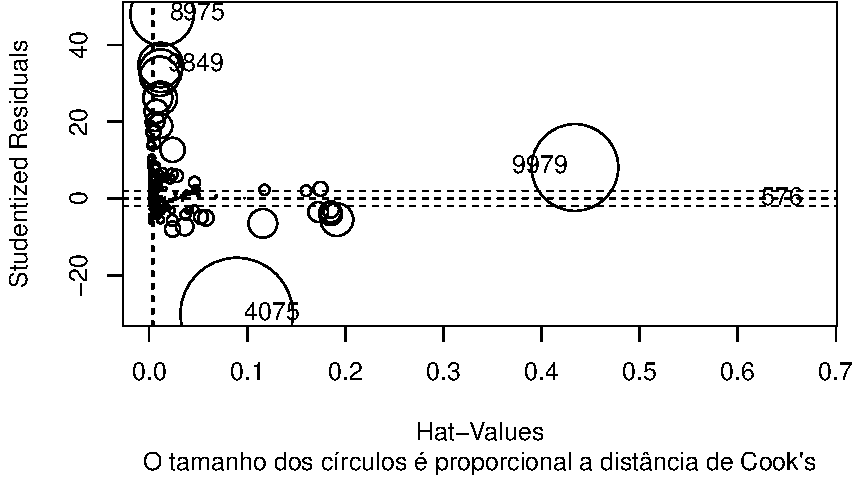
\includegraphics{12-exportedfigures/influence.plot-1} \end{center}
\vspace{-3mm}
\label{graf:influence}
\fonte{Desenvolvido a partir de dados coletados}
\vspace{-2mm}
\end{grafico}

O \autoref{graf:resstud} mostra a visualização entre os valores preditos em modelagem inicial versus o resíduos studentizados deletados do modelo. No \autoref{graf:histsp} é demonstrado de forma comparativa o histograma dos resíduos antes e após tratamento de dados e retirada dos outliers. 

\begin{grafico}
\vspace{20pt}
\caption{Resíduos studentizados vs Valores Preditos}
\vspace{-4mm}

\begin{center}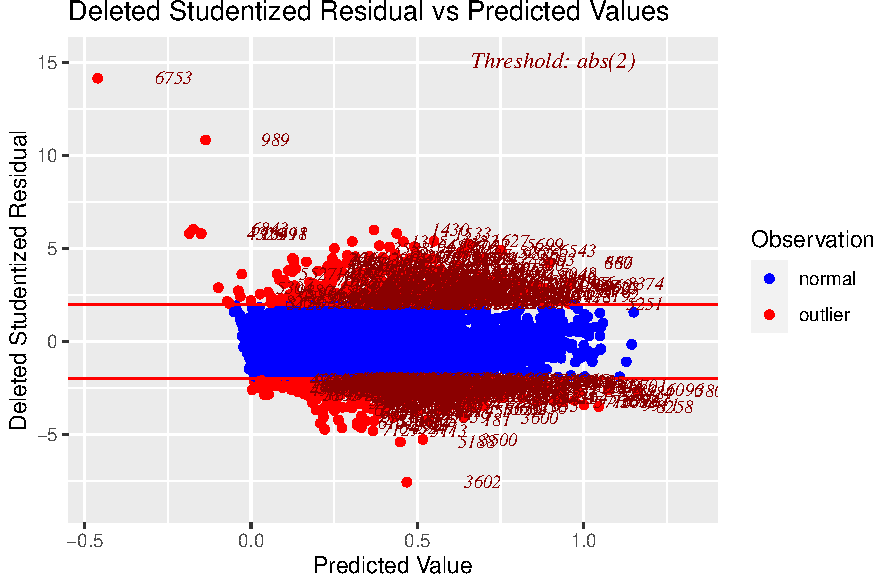
\includegraphics{12-exportedfigures/fit.01.graf-1} \end{center}
\vspace{-3mm}
\label{graf:resstud}
\fonte{Desenvolvido a partir da modelagem de dados}
\vspace{-2mm}
\end{grafico}

No \autoref{graf:histsp} é possível visualizar a distribuição de frequência da variável *Spread Ex-post* antes e após a retirada dos *outliers*.

\begin{grafico}[!hbtp]
\vspace{20pt}
\caption{Histograma demonstrando o ajuste na variável dependente}
\vspace{-4mm}

\begin{center}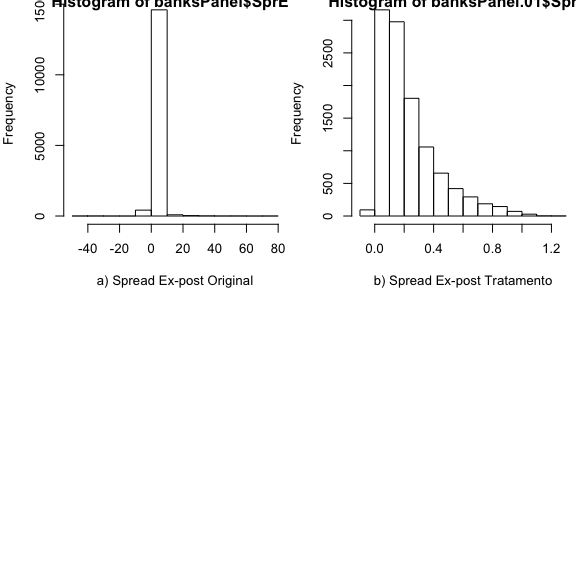
\includegraphics[width=1\linewidth]{12-exportedfigures/hist.SprEp-1} \end{center}
\vspace{3mm}
\label{graf:histsp}
\fonte{Desenvolvido a partir dos dados coletados}
\vspace{-2mm}
\end{grafico}

No \autoref{graf:histerr} é possível visualizar o comportamento de frequência dos resíduos antes e após a transformação dos dados.

\begin{grafico}[!hbtp]
\vspace{20pt}
\caption{Histograma dos Resíduos}
\vspace{-4mm}

\begin{center}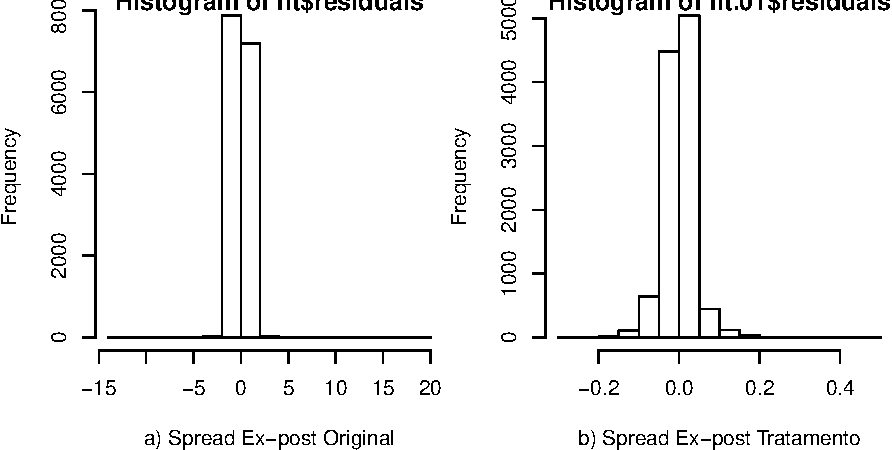
\includegraphics[width=1\linewidth]{12-exportedfigures/hist.residuals-1} \end{center}
\vspace{3mm}
\label{graf:histerr}
\fonte{Desenvolvido a partir dos dados coletados}
\vspace{-2mm}
\end{grafico}


No \autoref{graf:disperr} é possível visualizar o diagrama de dispersão entre os resíduos estudentizados e os valores preditos




\begin{grafico}[!hbtp]
\caption{Diagrama de Dispersão dos resíduos}
\vspace{-4mm}

\begin{center}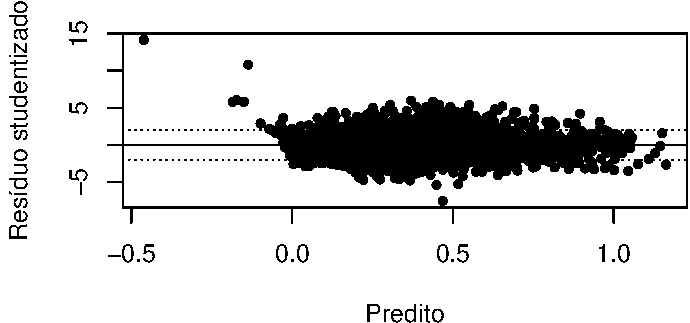
\includegraphics{12-exportedfigures/erros.disp-1} \end{center}
\vspace{3mm}
\label{graf:disperr}
\fonte{Desenvolvido a partir dos dados coletados}
\vspace{-2mm}
\end{grafico}











Entre as variáveis que foram eliminadas estão a participação de mercado ($MkSh$), grau de concentração ($GrCon$), operações de crédito total ($OpCrTotal$), *spread ex-ante* ($SprEa$) e o Índice de preços ao consumidor ($IPCA$), por possuírem elevada correlação com outras variáveis e por não se demonstrarem significativas em primeira testagem de modelo. 

Foram eliminadas as variáveis *dummy* de controle de capital ($OCap$) e caráter da instituição ($CrIns$), por falta de informações evolutivas. Somente a variável *dummy*  referente à taxonomia ($TpIns$) foi mantida no modelo, esperando que ela venha captar as diferenças operacionais.

O painel de dados foi modificado em algumas variáveis para se adequar a nova modelagem e evitar problemas de autocorrelação. Preliminarmente dos dados monetários foram escalonados para unidades em milhões. Para as variáveis referentes a base monetária e meios de pagamentos foram aplicados o logarítmo natural e de forma alternativa para fins de ajustes, considerado a variação ao longo do tempo destas variáveis.   

Foram incluídas no modelo variáveis  para captar as diferenças operacionais indicando a participação das receitas segmentadas em relação as receitas operacionais: receitas de operação de crédito ($ROpCr$), receitas de serviços ($RSrv$), receitas de participações ($RPart$) e outras receitas operacionais ($OtROp$).

Em relação a participação das modalidades de depósitos sobre as operações de créditos totais ($OpCrTot$), além dos dos depósitos a vista ($DepAv$) e depósito a prazo ($DepAp$),  foram incluídos os depósitos de poupança ($DepPop$), depósitos interfinanceiros ($DepIf$) e outros depósitos ($OtDep$). Com objetivos de verificar o perfil de captação por modalidade e como este influencia no nível de *spread*. 

Para a inadimplência ($Inad$) passou-se a usar a participação da provisão para crédito e outros créditos duvidoso sobre a soma das operações de crédito e outros crédito ($OpCrTot$)\footnote{Já adicionados dos próprios valores de provisão que se encontram subtraídos nas demonstrações contábeis}. 

Para captar as diferenças no perfil de despesas por modalidade de instituições e como este influencia no nível de *spread* além das despesas administrativas em função das operações totais ($DAdm$) foram incluídas as despesas de captação em função dos depósitos totais ($DesCap$) e outras despesas em função das operações de créditos totais ($OtDes$).

Finalizando os ajuste no modelo, foram incluídas as variáveis de impostos indiretos ($ImpInd$) e imposto de renda ($ImpRen$), completando as variáveis explícitas do *spread*, com exceção do compulsório por apresentar forte correlação com outras variáveis e do do fundo garantidor de crédito por se demonstrar insignificante.



\begin{equation}
\begin{aligned}
\operatorname{SprEp} &= \beta_{0} + \beta_{1}(\operatorname{DAdm}) + \beta_{2}(\operatorname{DesCap}) + \beta_{3}(\operatorname{GrCon})\ + \\
&\quad \beta_{4}(\operatorname{OtDes}) + \beta_{5}(\operatorname{Inad}) + \beta_{6}(\operatorname{Int}) + \beta_{7}(\operatorname{EPr})\ + \\
&\quad \beta_{8}(\operatorname{lnComp}) + \beta_{9}(\operatorname{ImpInd}) + \beta_{10}(\operatorname{ImpRend}) + \beta_{11}(\operatorname{DepAv})\ + \\
&\quad \beta_{12}(\operatorname{DepAp}) + \beta_{13}(\operatorname{DepPop}) + \beta_{14}(\operatorname{OpFin}) + \beta_{15}(\operatorname{OpEmp})\ + \\
&\quad \beta_{16}(\operatorname{ROpCr}) + \beta_{17}(\operatorname{RSrv}) + \beta_{18}(\operatorname{RPart}) + \beta_{19}(\operatorname{SelMet})\ + \\
&\quad \beta_{20}(\operatorname{VelMo}) + \epsilon
\end{aligned}
\end{equation}







<!--chapter:end:10-appendix-b.Rmd-->

\chapter{Modelos SUR}\label{apendicec}

\section{Metodologia}

O primeiro modelo a ser desenvolvido buscará testar e selecionar variáveis macroeconômicas e microeconômicas que exerçam significativa influência, de forma implícita e explícita no \emph{spread} bancário \emph{ex-post}. Partindo da concepção realizada no \autoref{apendicea}, conforme a \autoref{eq:oper02}.

Para a averiguação dos efeitos dos componentes do *spread ex-post* na rentabilidade das instituições bancárias serão utilizados modelos de regressão linear multivariada. Os modelos de regressão múltipla buscam, através de técnicas estatísticas e matemáticas, prever o comportamento de uma dada variável dependente, diante um conjunto de variáveis explanatórias \cite{hill:2010} \cite{gareth:2017}. 

\begin{equation}
Y = \beta_0 + \beta_1X_1 + \beta_2X_2...\beta_nX_n + \epsilon
\end{equation}

O modelo econométrico a ser utilizado será o método de dados em painel, denominado *Cross Section*, que combina séries temporais e dados em corte transversal. Este modelo busca captar diferenças individuais de comportamento, possibilitando combinar os dados para fins de estimação e inferência, posteriormente realizados testes de regressão e estimação \cite{hill:2010}.

\begin{equation}
y_{it} = \beta_{1it} + \beta_{2it}X_{2it} + \beta_{3it}X_{3it} + e_{it}
\end{equation}

O método *Cross Section* pode ser realizado por meio de três modelos de estimação que são: i) Modelo de regressão aparentemente não relacionadas (SUR); ii) Modelo de variável binárias — efeitos fixos — e iii) modelo de componentes estocásticos — efeitos aleatórios — \cite{hill:2010}. Serão testados os três métodos buscando selecionar o mais adequado ao modelo econométrico e ao conjunto de dados.

No modelo de regressão de dados aparentemente não relacionados — SUR —, os parâmetros dos diferentes grupos em corte transversal diferem entre si, porém são constantes ao longo do tempo. Os modelos podem ser estimados com suas funções de forma conjunta ou separada, onde esta última é indicada quando há correlação dos erros \cite{hill:2010}

\begin{equation}
y_{it} = \beta_{1it} + \beta_{2i}X_{2it} + \beta_{3i}X_{3it} + e_{it}
\end{equation}

\vspace{20pt}

No modelo de variável binárias — ou efeitos fixos —, o intercepto é abordado como um parâmetro desconhecido e fixo, onde as inferências são aplicadas somente ao cojunto de dados dos grupos do corte transversal do qual está disponível \cite{hill:2010}. 

\begin{equation}
y_{it} = \beta_{11}D_{1i} + \beta_{12}D_{2i} + ... + \beta_{1,10}D_{10i} + \beta_{2}X_{2it} + \beta_{3}X_{3it} + e_{it}
\end{equation}

\vspace{20pt}

O modelo de componentes estocásticos — ou efeitos aleatórios —, considera cada grupo do conjunto de dados como uma amostra aleatória de uma população maior, onde os interceptos são encarrados como resultados aleatórios da distribuição populacional de interceptos de grupos, realizando assim uma inferência da população de grupos \cite{hill:2010}.

\begin{equation}
y_{it} = \beta_{1i} + \beta_{2it}X_{2it} + \beta_{3it}X_{3it} + e_{it}
\end{equation}

Diante os pressupostos, o primeiro modelo irá verificar a influência das variações de variáveis componentes explícitas e implícitas do  *Spread Ex-post*, tendo no primeiro bloco variáveis microeconômicas e o segundo bloco as variáveis macroeconômicas, selecionando para o segundo modelo final somente as que apresentarem significância estatística.

\begin{equation}
\begin{aligned}
SprEp = &f(EPr, EAv, EAp, Atv, ImpInd, ImpId, \\ 
& Inad, MLq, DAdm, Jcp, MSh, HHI, TIns, OCap, \\ 
& CIns, Sel, Ipca, Comp, MPag, VMo, SprEa)
\end{aligned}
\end{equation}

Na construção do primeiro modelo econométrico serão adotadas simplificações para variáveis de resultado, eliminando as que possuem caráter constante, as obtidas por meio de resultado e por não possuírem dados, utilizando uma *proxy*.

\begin{equation}
\begin{aligned}
SprEp_{it} = & \beta_{0it} + \beta_{1it}EPr_{it} + \beta_{2it}EAv_{it} + \beta_{3it}EAp_{it} + \beta_{4it}DAdm_{it} + \beta_{5it}Vol_{it} + \\
& \beta_{6it}lnAtv_{it} + \beta_{7it}RC_{it} + \beta_{8it}MSh_{it} + \beta_{9it}HHI_{it} + \\ 
& \beta_{10it}Mod + \beta_{11it}OCap + \beta_{12it}SelOver_{t-1} + \beta_{13it}Ipca_{t-1} + \\
& \beta_{14it}Com_{t} + \beta_{15}Mpag_{t-1} + \beta_{16it}VMo_{t-1} +  \beta_{17t}SprEa_{t-1}
\end{aligned}
\end{equation}

O segundo modelo econométrico testará as variáveis implícitas e explícitas com significância estatística do primeiro modelo, atuando sobre a rentabilidade bancária $Rent$, conforme modelos especificados. Para a rentabilidade será considerada a razão entre o lucro líquido ($LcrLqd$) e a Receita das Operações de crédito ($RecOpCr$).

\begin{equation}
\begin{aligned}
Rent_{it} = & \beta_{0it} + \beta_{1it}EPr_{it} + \beta_{2it}EAv_{it} + \beta_{3it}EAp_{it} + \beta_{4it}DAdm_{it} + \beta_{5it}Vol_{it} + \\
& \beta_{6it}lnAtv_{it} + \beta_{7it}RC_{it} + \beta_{8it}MSh_{it} + \beta_{9it}HHI_{it} + \\ 
& \beta_{10it}Mod + \beta_{11it}OCap + \beta_{12it}SelOver_{t-1} + \beta_{13it}Ipca_{t-1} + \\
& \beta_{14it}Com_{t} + \beta_{15}Mpag_{t-1} + \beta_{16it}VMo_{t-1} +  \beta_{17t}SprEa_{t-1} + \epsilon_{t}
\end{aligned}
\end{equation}

Diante a definição dos modelos, seguem abaixo as hipóteses conceituais baseadas em concepções teóricas obtidas na pesquisa bibliográfica e das concepções desenvolvidas durante a pesquisa. O conjunto de hipóteses se apresenta na forma objetiva incluindo as expectativas para cada variável e contemplando os dois modelos construídos, com breve explanação sobre a mesma.


\section{Resultados}

Os dados em painel foram estimados nos métodos *pooling*, efeitos fixos e efeitos aleatórios, com os resultados demonstrados na \autoref{tb:modpool}, \autoref{tb:modef}, \autoref{tb:intfixef}, \autoref{tb:modrand} e \autoref{tb:modsr2}. 

\begin{table}[!htbp]
\caption{Resultado Modelo Pooling}
\vspace{1mm}
\begingroup\fontsize{10}{12}\selectfont

\begin{tabu} to \linewidth {>{\raggedright\arraybackslash}p{5cm}>{\raggedleft\arraybackslash}p{2cm}>{\raggedleft\arraybackslash}p{2cm}>{\raggedleft\arraybackslash}p{2cm}>{\raggedleft\arraybackslash}p{2cm}}
\toprule
  & Estimate & Std. Error & t-value & Pr(>|t|)\\
\midrule
\cellcolor{gray!6}{(Intercept)} & \cellcolor{gray!6}{-0.3092878} & \cellcolor{gray!6}{0.0993395} & \cellcolor{gray!6}{-3.1134419} & \cellcolor{gray!6}{0.0018540}\\
DAdm & 2.7021294 & 0.0256995 & 105.1432063 & 0.0000000\\
\cellcolor{gray!6}{DesCap} & \cellcolor{gray!6}{0.1835142} & \cellcolor{gray!6}{0.0172654} & \cellcolor{gray!6}{10.6289867} & \cellcolor{gray!6}{0.0000000}\\
GrCon & -0.2517865 & 0.0526275 & -4.7843107 & 0.0000017\\
\cellcolor{gray!6}{OtDes} & \cellcolor{gray!6}{2.0924644} & \cellcolor{gray!6}{0.0058786} & \cellcolor{gray!6}{355.9472529} & \cellcolor{gray!6}{0.0000000}\\
\addlinespace
Inad & 0.1272560 & 0.0090586 & 14.0481274 & 0.0000000\\
\cellcolor{gray!6}{Int} & \cellcolor{gray!6}{-0.8882561} & \cellcolor{gray!6}{0.1591881} & \cellcolor{gray!6}{-5.5799138} & \cellcolor{gray!6}{0.0000000}\\
EPr & -0.0485973 & 0.0007094 & -68.5069300 & 0.0000000\\
\cellcolor{gray!6}{TpInsBANCOS COMERCIAIS} & \cellcolor{gray!6}{0.0142915} & \cellcolor{gray!6}{0.0040990} & \cellcolor{gray!6}{3.4865420} & \cellcolor{gray!6}{0.0004912}\\
TpInsBANCOS DE DESENVOLVIMENTO & 0.0194829 & 0.0049261 & 3.9550083 & 0.0000770\\
\addlinespace
\cellcolor{gray!6}{TpInsBANCOS DE INVESTIMENTO} & \cellcolor{gray!6}{0.0225722} & \cellcolor{gray!6}{0.0044030} & \cellcolor{gray!6}{5.1265640} & \cellcolor{gray!6}{0.0000003}\\
TpInsBANCOS MULTIPLOS & 0.0179701 & 0.0038415 & 4.6778362 & 0.0000029\\
\cellcolor{gray!6}{TpInsBNDES} & \cellcolor{gray!6}{-0.0086736} & \cellcolor{gray!6}{0.0054035} & \cellcolor{gray!6}{-1.6051731} & \cellcolor{gray!6}{0.1084848}\\
TpInsCAIXA ECONOMICA FEDERAL & -0.0034413 & 0.0050080 & -0.6871573 & 0.4919983\\
\cellcolor{gray!6}{lnComp} & \cellcolor{gray!6}{0.0164127} & \cellcolor{gray!6}{0.0048572} & \cellcolor{gray!6}{3.3790268} & \cellcolor{gray!6}{0.0007300}\\
\addlinespace
ImpInd & -0.0051092 & 0.0023141 & -2.2078240 & 0.0272773\\
\cellcolor{gray!6}{ImpRend} & \cellcolor{gray!6}{0.2100251} & \cellcolor{gray!6}{0.0043978} & \cellcolor{gray!6}{47.7572308} & \cellcolor{gray!6}{0.0000000}\\
DepAv & 0.0136821 & 0.0027903 & 4.9034907 & 0.0000010\\
\cellcolor{gray!6}{DepAp} & \cellcolor{gray!6}{-0.0194386} & \cellcolor{gray!6}{0.0011597} & \cellcolor{gray!6}{-16.7615896} & \cellcolor{gray!6}{0.0000000}\\
DepPop & 0.0432018 & 0.0053479 & 8.0783290 & 0.0000000\\
\addlinespace
\cellcolor{gray!6}{OpFin} & \cellcolor{gray!6}{0.0116262} & \cellcolor{gray!6}{0.0019960} & \cellcolor{gray!6}{5.8247379} & \cellcolor{gray!6}{0.0000000}\\
OpEmp & 0.0189920 & 0.0022659 & 8.3818209 & 0.0000000\\
\cellcolor{gray!6}{ROpCr} & \cellcolor{gray!6}{-0.0065332} & \cellcolor{gray!6}{0.0021492} & \cellcolor{gray!6}{-3.0398161} & \cellcolor{gray!6}{0.0023729}\\
RSrv & 0.0069751 & 0.0059831 & 1.1657901 & 0.2437249\\
\cellcolor{gray!6}{RPart} & \cellcolor{gray!6}{0.2351028} & \cellcolor{gray!6}{0.0112137} & \cellcolor{gray!6}{20.9657128} & \cellcolor{gray!6}{0.0000000}\\
\addlinespace
SelMet & 0.0993112 & 0.0158476 & 6.2666460 & 0.0000000\\
\cellcolor{gray!6}{VelMo} & \cellcolor{gray!6}{-0.1413806} & \cellcolor{gray!6}{0.0333750} & \cellcolor{gray!6}{-4.2361259} & \cellcolor{gray!6}{0.0000229}\\
\bottomrule
\end{tabu}
\endgroup{}
\vspace{1mm}
\label{tb:modpool}
\fonte{Desenvolvido a partir dos dados coletados}
\vspace{-2mm}
\end{table}

\begin{table}[!htb]
\caption{Resultado Modelo Efeitos Fixos}
\vspace{1mm}
\begingroup\fontsize{10}{12}\selectfont

\begin{tabu} to \linewidth {>{\raggedright\arraybackslash}p{5cm}>{\raggedleft\arraybackslash}p{2cm}>{\raggedleft\arraybackslash}p{2cm}>{\raggedleft\arraybackslash}p{2cm}>{\raggedleft\arraybackslash}p{2cm}}
\toprule
  & Estimate & Std. Error & t-value & Pr(>|t|)\\
\midrule
\cellcolor{gray!6}{DAdm} & \cellcolor{gray!6}{2.7040771} & \cellcolor{gray!6}{0.0257065} & \cellcolor{gray!6}{105.190515} & \cellcolor{gray!6}{0.0000000}\\
DesCap & 0.1843886 & 0.0172654 & 10.679651 & 0.0000000\\
\cellcolor{gray!6}{GrCon} & \cellcolor{gray!6}{-0.2514115} & \cellcolor{gray!6}{0.0526161} & \cellcolor{gray!6}{-4.778225} & \cellcolor{gray!6}{0.0000018}\\
OtDes & 2.0908117 & 0.0059170 & 353.355982 & 0.0000000\\
\cellcolor{gray!6}{Inad} & \cellcolor{gray!6}{0.1296956} & \cellcolor{gray!6}{0.0091128} & \cellcolor{gray!6}{14.232294} & \cellcolor{gray!6}{0.0000000}\\
\addlinespace
Int & -0.9208187 & 0.1597233 & -5.765085 & 0.0000000\\
\cellcolor{gray!6}{EPr} & \cellcolor{gray!6}{-0.0485227} & \cellcolor{gray!6}{0.0007099} & \cellcolor{gray!6}{-68.352221} & \cellcolor{gray!6}{0.0000000}\\
lnComp & 0.0165243 & 0.0048564 & 3.402618 & 0.0006698\\
\cellcolor{gray!6}{ImpInd} & \cellcolor{gray!6}{-0.0052058} & \cellcolor{gray!6}{0.0023140} & \cellcolor{gray!6}{-2.249702} & \cellcolor{gray!6}{0.0244878}\\
ImpRend & 0.2104211 & 0.0043998 & 47.824629 & 0.0000000\\
\addlinespace
\cellcolor{gray!6}{DepAv} & \cellcolor{gray!6}{0.0128900} & \cellcolor{gray!6}{0.0028089} & \cellcolor{gray!6}{4.589000} & \cellcolor{gray!6}{0.0000045}\\
DepAp & -0.0199056 & 0.0011755 & -16.934022 & 0.0000000\\
\cellcolor{gray!6}{DepPop} & \cellcolor{gray!6}{0.0438550} & \cellcolor{gray!6}{0.0053535} & \cellcolor{gray!6}{8.191810} & \cellcolor{gray!6}{0.0000000}\\
OpFin & 0.0255071 & 0.0060862 & 4.190956 & 0.0000280\\
\cellcolor{gray!6}{OpEmp} & \cellcolor{gray!6}{0.0330548} & \cellcolor{gray!6}{0.0062501} & \cellcolor{gray!6}{5.288675} & \cellcolor{gray!6}{0.0000001}\\
\addlinespace
OtOp & 0.0148767 & 0.0061623 & 2.414158 & 0.0157880\\
\cellcolor{gray!6}{ROpCr} & \cellcolor{gray!6}{-0.0067937} & \cellcolor{gray!6}{0.0021514} & \cellcolor{gray!6}{-3.157721} & \cellcolor{gray!6}{0.0015944}\\
RSrv & 0.0055269 & 0.0060118 & 0.919338 & 0.3579392\\
\cellcolor{gray!6}{RPart} & \cellcolor{gray!6}{0.2332148} & \cellcolor{gray!6}{0.0112384} & \cellcolor{gray!6}{20.751531} & \cellcolor{gray!6}{0.0000000}\\
SelMet & 0.0991463 & 0.0158442 & 6.257570 & 0.0000000\\
\addlinespace
\cellcolor{gray!6}{VelMo} & \cellcolor{gray!6}{-0.1414248} & \cellcolor{gray!6}{0.0333676} & \cellcolor{gray!6}{-4.238391} & \cellcolor{gray!6}{0.0000227}\\
\bottomrule
\end{tabu}
\endgroup{}
\vspace{1mm}
\label{tb:modef}
\fonte{Desenvolvido a partir dos dados coletados}
\vspace{-2mm}
\end{table}


\begin{table}[!hbtp]
\caption{Interceptos do modelo de Efeitos Fixos}
\vspace{1mm}
\begingroup\fontsize{10}{12}\selectfont

\begin{tabu} to \linewidth {>{\raggedright\arraybackslash}p{5cm}>{\raggedleft\arraybackslash}p{2cm}>{\raggedleft\arraybackslash}p{2cm}>{\raggedleft\arraybackslash}p{2cm}>{\raggedleft\arraybackslash}p{2cm}}
\toprule
  & Estimate & Std. Error & t-value & Pr(>|t|)\\
\midrule
\cellcolor{gray!6}{BANCO DO BRASIL} & \cellcolor{gray!6}{-0.3252951} & \cellcolor{gray!6}{0.0995386} & \cellcolor{gray!6}{-3.268031} & \cellcolor{gray!6}{0.0010863}\\
BANCOS COMERCIAIS & -0.3108937 & 0.0994296 & -3.126772 & 0.0017720\\
\cellcolor{gray!6}{BANCOS DE DESENVOLVIMENTO} & \cellcolor{gray!6}{-0.3046604} & \cellcolor{gray!6}{0.0994253} & \cellcolor{gray!6}{-3.064215} & \cellcolor{gray!6}{0.0021878}\\
BANCOS DE INVESTIMENTO & -0.3025806 & 0.0994144 & -3.043630 & 0.0023430\\
\cellcolor{gray!6}{BANCOS MULTIPLOS} & \cellcolor{gray!6}{-0.3071196} & \cellcolor{gray!6}{0.0994550} & \cellcolor{gray!6}{-3.088027} & \cellcolor{gray!6}{0.0020200}\\
\addlinespace
BNDES & -0.3339169 & 0.0995302 & -3.354931 & 0.0007966\\
\cellcolor{gray!6}{CAIXA ECONOMICA FEDERAL} & \cellcolor{gray!6}{-0.3277114} & \cellcolor{gray!6}{0.0995675} & \cellcolor{gray!6}{-3.291349} & \cellcolor{gray!6}{0.0010003}\\
\bottomrule
\end{tabu}
\endgroup{}
\vspace{1mm}
\label{tb:intfixef}
\fonte{Desenvolvido a partir dos dados coletados}
\vspace{-2mm}
\end{table}

\begin{table}[!htbp]
\caption{Resultado Modelo Efeitos Aleatórios}
\vspace{1mm}
\begingroup\fontsize{10}{12}\selectfont

\begin{tabu} to \linewidth {>{\raggedright\arraybackslash}p{5cm}>{\raggedleft\arraybackslash}p{2cm}>{\raggedleft\arraybackslash}p{2cm}>{\raggedleft\arraybackslash}p{2cm}>{\raggedleft\arraybackslash}p{2cm}}
\toprule
  & Estimate & Std. Error & z-value & Pr(>|z|)\\
\midrule
\cellcolor{gray!6}{(Intercept)} & \cellcolor{gray!6}{-0.3092878} & \cellcolor{gray!6}{0.0993407} & \cellcolor{gray!6}{-3.1134051} & \cellcolor{gray!6}{0.0018494}\\
DAdm & 2.7021294 & 0.0256995 & 105.1432063 & 0.0000000\\
\cellcolor{gray!6}{DesCap} & \cellcolor{gray!6}{0.1835142} & \cellcolor{gray!6}{0.0172654} & \cellcolor{gray!6}{10.6289867} & \cellcolor{gray!6}{0.0000000}\\
GrCon & -0.2517865 & 0.0526275 & -4.7843107 & 0.0000017\\
\cellcolor{gray!6}{OtDes} & \cellcolor{gray!6}{2.0924644} & \cellcolor{gray!6}{0.0058786} & \cellcolor{gray!6}{355.9472529} & \cellcolor{gray!6}{0.0000000}\\
\addlinespace
Inad & 0.1272560 & 0.0090586 & 14.0481274 & 0.0000000\\
\cellcolor{gray!6}{Int} & \cellcolor{gray!6}{-0.8882561} & \cellcolor{gray!6}{0.1591881} & \cellcolor{gray!6}{-5.5799138} & \cellcolor{gray!6}{0.0000000}\\
EPr & -0.0485973 & 0.0007094 & -68.5069300 & 0.0000000\\
\cellcolor{gray!6}{TpInsBANCOS COMERCIAIS} & \cellcolor{gray!6}{0.0142915} & \cellcolor{gray!6}{0.0041556} & \cellcolor{gray!6}{3.4390892} & \cellcolor{gray!6}{0.0005837}\\
TpInsBANCOS DE DESENVOLVIMENTO & 0.0194829 & 0.0049733 & 3.9175032 & 0.0000895\\
\addlinespace
\cellcolor{gray!6}{TpInsBANCOS DE INVESTIMENTO} & \cellcolor{gray!6}{0.0225722} & \cellcolor{gray!6}{0.0044557} & \cellcolor{gray!6}{5.0659266} & \cellcolor{gray!6}{0.0000004}\\
TpInsBANCOS MULTIPLOS & 0.0179701 & 0.0039018 & 4.6055519 & 0.0000041\\
\cellcolor{gray!6}{TpInsBNDES} & \cellcolor{gray!6}{-0.0086736} & \cellcolor{gray!6}{0.0054465} & \cellcolor{gray!6}{-1.5924916} & \cellcolor{gray!6}{0.1112743}\\
TpInsCAIXA ECONOMICA FEDERAL & -0.0034413 & 0.0050544 & -0.6808494 & 0.4959668\\
\cellcolor{gray!6}{lnComp} & \cellcolor{gray!6}{0.0164127} & \cellcolor{gray!6}{0.0048572} & \cellcolor{gray!6}{3.3790268} & \cellcolor{gray!6}{0.0007274}\\
\addlinespace
ImpInd & -0.0051092 & 0.0023141 & -2.2078240 & 0.0272565\\
\cellcolor{gray!6}{ImpRend} & \cellcolor{gray!6}{0.2100251} & \cellcolor{gray!6}{0.0043978} & \cellcolor{gray!6}{47.7572308} & \cellcolor{gray!6}{0.0000000}\\
DepAv & 0.0136821 & 0.0027903 & 4.9034907 & 0.0000009\\
\cellcolor{gray!6}{DepAp} & \cellcolor{gray!6}{-0.0194386} & \cellcolor{gray!6}{0.0011597} & \cellcolor{gray!6}{-16.7615896} & \cellcolor{gray!6}{0.0000000}\\
DepPop & 0.0432018 & 0.0053479 & 8.0783290 & 0.0000000\\
\addlinespace
\cellcolor{gray!6}{OpFin} & \cellcolor{gray!6}{0.0116262} & \cellcolor{gray!6}{0.0019960} & \cellcolor{gray!6}{5.8247379} & \cellcolor{gray!6}{0.0000000}\\
OpEmp & 0.0189920 & 0.0022659 & 8.3818209 & 0.0000000\\
\cellcolor{gray!6}{ROpCr} & \cellcolor{gray!6}{-0.0065332} & \cellcolor{gray!6}{0.0021492} & \cellcolor{gray!6}{-3.0398161} & \cellcolor{gray!6}{0.0023672}\\
RSrv & 0.0069751 & 0.0059831 & 1.1657901 & 0.2436993\\
\cellcolor{gray!6}{RPart} & \cellcolor{gray!6}{0.2351028} & \cellcolor{gray!6}{0.0112137} & \cellcolor{gray!6}{20.9657128} & \cellcolor{gray!6}{0.0000000}\\
\addlinespace
SelMet & 0.0993112 & 0.0158476 & 6.2666460 & 0.0000000\\
\cellcolor{gray!6}{VelMo} & \cellcolor{gray!6}{-0.1413806} & \cellcolor{gray!6}{0.0333750} & \cellcolor{gray!6}{-4.2361259} & \cellcolor{gray!6}{0.0000227}\\
\bottomrule
\end{tabu}
\endgroup{}
\vspace{1mm}
\label{tb:modrand}
\fonte{Desenvolvido a partir dos dados coletados}
\vspace{-2mm}
\end{table}

\vspace{20pt}

\begin{table}[!hbtp]
\caption{Resultado de coeficiente de determinação para os modelos}
\vspace{1mm}
\begingroup\fontsize{10}{12}\selectfont

\begin{tabu} to \linewidth {>{\raggedright}X>{\raggedleft}X>{\raggedleft}X}
\toprule
Modelos & R.2 & R.Ajustado\\
\midrule
\cellcolor{gray!6}{Pooling} & \cellcolor{gray!6}{0.9663854} & \cellcolor{gray!6}{0.9663050}\\
Efeitos Fixos & 0.9657173 & 0.9656322\\
\cellcolor{gray!6}{Efeitos Aleatórios} & \cellcolor{gray!6}{0.9663317} & \cellcolor{gray!6}{0.9662512}\\
\bottomrule
\end{tabu}
\endgroup{}
\vspace{1mm}
\label{tb:modsr2}
\fonte{Desenvolvido a partir dos dados coletados}
\vspace{-2mm}
\end{table}






No modelo \emph{pooling}, não foi encontrada significância a 5%, para as variáveis de meios de pagamentos ($M4$), velocidade da moeda ($VelMo$), impostos indiretos ($ImpInd$) e depósitos a vista ($DepAv$). As demais variáveis apresentação elevado nível de significância. Foi aplicado o teste de Wooldridge aceitando a hipótese nula que os erros para a taxonomia não são relacionados.  

Foi utilizado o teste Wooldridge para o modelo \emph{pooling} para checar a correlação nos erros no grupo de taxonomia. O resultado do teste conforme \autoref{tb:wdtest} aceita a hipotese nula, indicando que os erros entre o grupo avaliado não são correlacionados.

\vspace{20pt}

\begin{table}[!hbtp]
\caption{Resultado do teste Wooldridge para o modelo pooling}
\vspace{1mm}
\begingroup\fontsize{10}{12}\selectfont

\begin{tabu} to \linewidth {>{\raggedright}X>{\raggedleft}X>{\raggedleft}X>{\raggedright}X}
\toprule
  & Estatística & Valor.P & Hipótese.Alternativa\\
\midrule
\cellcolor{gray!6}{z} & \cellcolor{gray!6}{-1.184752} & \cellcolor{gray!6}{0.2361154} & \cellcolor{gray!6}{Correlação nos Erros}\\
\bottomrule
\end{tabu}
\endgroup{}
\vspace{1mm}
\label{tb:wdtest}
\fonte{Desenvolvido a partir dos dados estimados}
\vspace{-2mm}
\end{table}




Para comparação entre os modelos pooling e efeitos fixos foi aplicado o teste F de Chrow para avaliar os efeitos individuais, sendo rejeitada a hipótese nula de igualdade nos interceptos e coeficientes, indicando que o modelo de efeitos fixos seria mais adequado para estimação do modelo. 

\vspace{20pt}

\begin{table}[!hbtp]
\caption{Teste F para igualdade nos interceptos e inclinações}
\vspace{1mm}
\begingroup\fontsize{10}{12}\selectfont

\begin{tabu} to \linewidth {>{\raggedright}X>{\raggedleft}X>{\raggedleft}X>{\raggedleft}X>{\raggedleft}X>{\raggedright}X}
\toprule
  & Estatística & DF01 & DF02 & P.Valor & Hipótese.Alternativa\\
\midrule
\cellcolor{gray!6}{F} & \cellcolor{gray!6}{5.825573} & \cellcolor{gray!6}{-1} & \cellcolor{gray!6}{10870} & \cellcolor{gray!6}{NaN} & \cellcolor{gray!6}{Não Igualdade nos Interceptos}\\
\bottomrule
\end{tabu}
\endgroup{}
\vspace{-1mm}
\label{tb:pftest}
\fonte{Desenvolvido a partir dos dados estimados}
\vspace{-2mm}
\end{table}

Para comparar os modelos pooling e efeitos aleatórios foi utilizado o teste Breusch-Pagan (multiplicador de lagrange) para modelos em painel não balanceados, aceitando a hipótese nula que a variância dos erros são iguais, indicando homocedasticidade.  

\vspace{20pt}

\begin{table}[!hbtp]
\caption{Teste Breusch-Pagan para variância dos erros em painéis desbalanceados}
\vspace{1mm}
\begingroup\fontsize{10}{12}\selectfont

\begin{tabu} to \linewidth {>{\raggedright}X>{\raggedleft}X>{\raggedleft}X>{\raggedleft}X>{\raggedright}X}
\toprule
  & Estatística & Df & P.Valor & Alternativa\\
\midrule
\cellcolor{gray!6}{chisq} & \cellcolor{gray!6}{0.7101622} & \cellcolor{gray!6}{1} & \cellcolor{gray!6}{0.39939} & \cellcolor{gray!6}{Variância dos Erros}\\
\bottomrule
\end{tabu}
\endgroup{}
\vspace{-1mm}
\label{tb:lbptest}
\fonte{Desenvolvido a partir dos dados estimados}
\vspace{-2mm}
\end{table}

Em termos de comparação entre os modelos de efeitos fixos e efeitos aleatórios foi utilizado o teste de Hausman, com rejeição da hipotese nula (parâmetros não correlacionados), indicando assim correlação entre os parâmetros e indicando que o modelo e efeitos fixos é mais adequado para avaliação do modelo.   

\begin{table}[!hbtp]
\caption{Teste Hausman para correlação dos parâmetros}
\vspace{1mm}
\begingroup\fontsize{10}{12}\selectfont

\begin{tabu} to \linewidth {>{\raggedright}X>{\raggedleft}X>{\raggedleft}X>{\raggedleft}X>{\raggedright}X}
\toprule
  & Estatística & DF & Valor.P & Alternativa\\
\midrule
\cellcolor{gray!6}{chisq} & \cellcolor{gray!6}{5.828301} & \cellcolor{gray!6}{20} & \cellcolor{gray!6}{0.9991103} & \cellcolor{gray!6}{Correlação nos Parâmetros}\\
\bottomrule
\end{tabu}
\endgroup{}
\vspace{-1mm}
\label{tb:htest}
\fonte{Desenvolvido a partir dos dados estimados}
\vspace{-2mm}
\end{table}

Para checar a dependência transversal do modelo de efeitos fixo foi utilizado o teste Pesaran, sendo rejeitada a hipótese nula (não correlação dos resíduos aos indivíduos) indicando que os resíduos entre os indivíduos estão correlacionados.

\begin{table}[!hbtp]
\caption{Teste Persan CD para dependência transversal}
\vspace{1mm}
\begingroup\fontsize{10}{12}\selectfont

\begin{tabu} to \linewidth {>{\raggedright}X>{\raggedleft}X>{\raggedleft}X>{\raggedright}X}
\toprule
Modelo & Estatística & Valor.P & Alternativa\\
\midrule
\cellcolor{gray!6}{Pooling} & \cellcolor{gray!6}{1.0691444} & \cellcolor{gray!6}{0.2850046} & \cellcolor{gray!6}{Correlação nos resíduos dos indivíduos}\\
Efeitos Fixos & 1.0691444 & 0.3365134 & Correlação nos resíduos dos indivíduos\\
\cellcolor{gray!6}{Efeitos Aleatórios} & \cellcolor{gray!6}{0.9610772} & \cellcolor{gray!6}{0.2850046} & \cellcolor{gray!6}{Correlação nos resíduos dos indivíduos}\\
\bottomrule
\end{tabu}
\endgroup{}
\vspace{-1mm}
\label{tb:pcdtest}
\fonte{Desenvolvido a partir dos dados estimados}
\vspace{-2mm}
\end{table}


A normalidade dos resíduos os três modelos foi testado pelo método Shapiro-Wilk, rejeitando a hipótese nula de normalidade dos resíduos, indicando que os modelo apresenta problemas de hetetocedasticidadade. 

\begin{table}[!hbtp]
\caption{Teste Shapiro-Wilk para normalidade dos resíduos}
\vspace{1mm}
\begingroup\fontsize{10}{12}\selectfont

\begin{tabu} to \linewidth {>{\raggedright}X>{\raggedleft}X>{\raggedleft}X}
\toprule
Modelo & Estatística.W & Valor.P\\
\midrule
\cellcolor{gray!6}{Pooling} & \cellcolor{gray!6}{0.961418} & \cellcolor{gray!6}{0}\\
Efeitos Fixos & 0.961288 & 0\\
\cellcolor{gray!6}{Efeitos Aleatórios} & \cellcolor{gray!6}{0.961418} & \cellcolor{gray!6}{0}\\
\bottomrule
\end{tabu}
\endgroup{}
\vspace{-1mm}
\label{tb:swtest}
\fonte{Desenvolvido a partir dos dados estimados}
\vspace{-2mm}
\end{table}

A normalidade dos resíduos do modelo de efeitos aleatórios foi testado pelo método, rejeitando a hipótese nula de normalidade dos resíduos, indicando que o modelo apresenta problemas de hetetocedasticidadade. 

\begin{table}[!hbtp]
\caption{Teste Breusch-Pagan estudentizado para normalidade dos resíduos em efeitos aleatórios}
\vspace{1mm}
\begingroup\fontsize{10}{12}\selectfont

\begin{tabu} to \linewidth {>{\raggedright}X>{\raggedleft}X>{\raggedleft}X}
\toprule
Modelo & Estatística & Valor.P\\
\midrule
\cellcolor{gray!6}{Pooling} & \cellcolor{gray!6}{2081.419} & \cellcolor{gray!6}{0}\\
Efeitos Fixos & 2070.384 & 0\\
\cellcolor{gray!6}{Efeitos Aleatórios} & \cellcolor{gray!6}{2081.419} & \cellcolor{gray!6}{0}\\
\bottomrule
\end{tabu}
\endgroup{}
\vspace{-1mm}
\label{tb:sbptest}
\fonte{Desenvolvido a partir dos dados estimados}
\vspace{-2mm}
\end{table}

Foi testada a correlação serial do modelo de efeitos fixos, rejeitando a hipotese nula (de não correlação serial), indicando assim que o painel de dados possui problemas de correlação serial entre dos dados. 

\begin{table}[!hbtp]
\caption{Teste Breusch-Godfrey/Wooldridge para correlação serial}
\vspace{1mm}
\begingroup\fontsize{10}{12}\selectfont

\begin{tabu} to \linewidth {>{\raggedright}X>{\raggedleft}X>{\raggedleft}X>{\raggedleft}X>{\raggedright}X}
\toprule
Modelos & Estatística & DF & Valor.P & Alternativa\\
\midrule
\cellcolor{gray!6}{Pooling} & \cellcolor{gray!6}{399.0382} & \cellcolor{gray!6}{101} & \cellcolor{gray!6}{0} & \cellcolor{gray!6}{Correlação serial no erros indissiocráticos}\\
Efeitos Fixos & 400.0635 & 101 & 0 & Correlação serial no erros indissiocráticos\\
\cellcolor{gray!6}{Efeitos Aleatórios} & \cellcolor{gray!6}{399.0382} & \cellcolor{gray!6}{101} & \cellcolor{gray!6}{0} & \cellcolor{gray!6}{Correlação serial no erros indissiocráticos}\\
\bottomrule
\end{tabu}
\endgroup{}
\vspace{-1mm}
\label{tb:bgwtest}
\fonte{Desenvolvido a partir dos dados estimados}
\vspace{-2mm}
\end{table}

Os resultados das estimações dos modelos, demonstraram elevada significância para as variáveis, com coeficientes de determinação acima em torno de 95%, porém os testes indicaram problemas de heterocedasticidade e correlação serial dos dados, podendo estar inflando os resultados, demonstrando-se inadequados para uma estimação confiável. 


\end{apendicesenv}

\}\{
\}

\ifthenelse{\equal{\terAnexo}{Sim}}{
\begin{anexosenv}

\renewcommand{\arabic{chapter}}{\arabic{chapter}}
        
\chapter{Cálculo Resultados}

\lipsum[31] 

\lipsum[32] 

\end{anexosenv}
}{}

\ifthenelse{\equal{\terIndiceR}{Sim}}{
\phantompart
\printindex
}{}

\printbibliography

\end{document}
